% LTeX: language=zh-CN
\chapter{二维材料异质结生长机理的研究}
\section{引言}
石墨烯作为经典的二维材料,由于独特的晶体结构和电子结构特性,在超导,量子计算、量子晶体管等方面具有独特的优势\citing{RN1068-2020,RN1071-2021,RN1065-2013,RN997-2007,RN1008-2015}。而要将石墨烯真正运用到器件之中,与现行的平面硅工艺兼容,研究者需要将石墨烯转移到\cemb{SiO2}等绝缘衬底的表面。而石墨烯在\cemb{SiO2}为代表的绝缘衬底表面通常以无序的状态存在,破碎的晶格大幅度的消弱了石墨烯在这些绝缘衬底表面的电子性质。
而作为二维材料中的绝缘体,六方氮化硼\cemb{h-BN}具有较大的带隙同时也保有二维材料高质量的面内结构。趋近完美的二维晶体结构使得\cemb{h-BN}在禁带内具有极低的缺陷态密度以及较高的击穿电压。同时,\cemb{h-BN}与石墨烯之间的晶格失配只有\SI{2}{\percent},使得\cemb{h-BN}非常适合在高性能电子器件中替代\cemb{SiO2}作为石墨烯的衬底材料 \citing{RN959-2010}。这种将不同的二维材料纵向堆叠起来可以制成纵向异质结,许多新奇的物理现象已经在石墨烯和\cemb{h-BN}的二维异质结中被发现,如在外磁场下的霍夫斯塔特电子-场强蝴蝶分型图像\citing{RN1286-2013, RN1287-2013, RN1285-2013}。从生产的角度,石墨烯/\cemb{h-BN}纵向二维异质结具有非常好的制备质量,同时保持了石墨烯高度可调的物理特性。这些都使得石墨烯/\cemb{h-BN}纵向二维异质结成为了一个非常好的观测新奇量子现象的基础平台。

常用于大规模低成本制备石墨烯的化学气相沉积法通常需要\cemb{Cu}等金属衬底的催化作用的协助。由于\cemb{h-BN}对于甲烷等含碳前驱体裂解反应的催化活性远不及金属衬底,石墨烯在\cemb{h-BN}上直接生长的速率同样也远低于在金属衬底上的生长速率。因此,一些研究者试图通过增加前驱体裂解速率的方式提升纵向二维异质结的合成效率。例如,在2015年,研究者通过添加作为气体催化剂的硅烷等方式,提高石墨烯在\cemb{h-BN}表面的生长速率\citing{RN1059-2015}。但以上方式通常使用较高的生长温度或者使用等离子体辅助的方式进行生长石墨烯。在这种情况下,虽然石墨烯能够在\cemb{h-BN}的表面生长,但是高温会破坏\cemb{h-BN}生长所需的金属衬底。因此我们需要寻找到一种生长流程,使得温度维持在金属衬底能够生长\cemb{h-BN}能够的同时尽可能的加快石墨烯在\cemb{h-BN}表面的生长速率。

在\ref{cap:CG}章中,我们构建了一种利用\cemb{Cu}蒸气近邻催化效应在\cemb{h-BN}表面直接堆叠生长石墨烯的方法。该方法利用从外缘\cemb{Cu}源处蒸发而出的\cemb{Cu}蒸气作为催化剂,在\cemb{h-BN}的表面产生对\cemb{CH4}的近邻催化效应,加速甲烷在\cemb{h-BN}表面的裂解,从而达到加速\cemb{h-BN}表面石墨烯生长的目的。利用理论计算的方法,我们证明了\cemb{Cu}蒸气从蒸发源到达\cemb{h-BN}表面并进行\cemb{CH4}裂解催化的可行性,同时给出了裂解而成的\cemb{C}原子在\cemb{h-BN}表面成核生长成石墨烯的生长序列。我们认为通过这种直接堆叠生长的方法能够能够实现石墨烯/\cemb{h-BN}的双层以及多层堆叠交替大规模生长,进一步提升石墨烯/\cemb{h-BN}二维纵向异质结在高性能电子器件应用的可行性,推进石墨烯/\cemb{h-BN}二维纵向异质结的工程化和集成化。

二维材料的另一种形成异质结的方式是在平面内进行拼接,形成横向二维异质结。同时,横向二维异质结中的一维形式的边沿接触能够在界面原子的尺度内提供非常小的接触面积和较低的接触阻抗\citing{RN1284-2014}。同时,在横向二维材料异质结中,由于界面原子之间通常为共价键或者离子键键合,没有纵向二维异质结中以范德华作用相连接的原子层间间隙,边沿接触为二维材料的载流子注入提供了可能。

过渡族金属硫族化合物(TMDs)是一类由过渡金属(\cemb{Ti}、\cemb{V}、\cemb{Mo}等)过渡族金属元素和硫族元素(\cemb{S}、\cemb{Se}等)所组成的层状材料。此类材料具有宽泛的带隙范围和能带结构,可以组合出具有多种能带匹配的的二维半导体异质结,被认为可以在包括包括发光二极管,单极、双极型电子器件,隧穿场效应管高性能电子、光电子器件中发挥广泛的作用\citing{RN957-2016, RN958-2018}。过渡族金属硫族化合物的二维化会导致过渡族金属硫族化合物的电子性质产生有趣的变化。如\cemb{MoS2}、\cemb{WS2}、\cemb{WSe2}等材料经过二维化后,电子结构由在块体状态下的间接带隙变为的直接带隙\citing{RN984-2010,RN985-2013,RN986-2015}。\cemb{MoS2}在二维化之后表现出栅极诱导的超导态\citing{RN1304-2016}。

\cemb{VSe2}是一种典型的过渡族金属硫族化合物材料,单层的\cemb{VSe2}表现出本征的磁有序电子结构,被研究者认为是一种少见的磁性二维材料\citing{RN1318-2018, RN1320-2018, RN1321-2020, RN1319-2018}。在\cemb{VSe2}中,\cemb{V4+}离子中3d轨道仅有一个电子。这个未配对的电子使得\cemb{VSe2}具有许多电子自旋相关的特性。相邻的\cemb{V-V}原子对之间强烈的电子耦合导致了电流密度波(Current density wave, CDW)的存在。同时,不同于其他磁性二维材料,磁性\cemb{VSe2}具有高于室温的居里温度。单层的的\cemb{VSe2}的距离温度高达\SI{470}{\kelvin}\citing{RN1322-2019},显著高于\cemb{CrI3}、\cemb{Fe3GeTe2}等二维磁性材料\citing{RN1325-2017, RN1326-2018}。

通常来说,在金半接触界面的肖特基势垒会导致载流子的输运受到抑制。与传统的\cemb{Au}等金属电极相比,石墨烯拥有非常低的功函数。因此通过将石墨烯与\cemb{VSe2}等过渡金属硫化物二维材料相连接可以实现非常低的小肖特基势垒,提升二维电子器件的载流子输运性能。

在\ref{cap:VS}章中,使用密度泛函理论计算,我们对石墨烯/\cemb{VSe2}横向异质结的构建进行了初步的探索。我们的研究发现在具有台阶的少层石墨烯表面,\cemb{VSe2}的生长具有石墨烯台阶层数的选择性。单层的\cemb{VSe2}更加倾向于在双层的石墨烯台阶的边缘生长。单层的\cemb{VSe2}在双层石墨烯台阶处的选择性生长有利于推动石墨烯/\cemb{VSe2}横向异质结的大规模制备,进一步提升石墨烯/\cemb{VSe2}二维横向异质结在高性能电子器件应用的可行性,推进石墨烯/\cemb{VSe2}二维横向异质结的工程化和集成化。

\section{计算细节}

在本章中密度泛函理论主要使用Vienna ab-initio Simulation Package (VASP) 软件包进行计算。在密度泛函理论计算中,我们使用广义梯度近似(GGA)下的 Perdew-Burke-Ernzerhof (PBE)泛函描述电子之间的交换关联作用。平面波的截断动能取为为$\SI{500}{\electronvolt}$。为了研究\cemb{Cu}/\cemb{h-BN}衬底表面石墨烯的生长情况,我们采用切片模型并在垂直表面方向放置至少$\SI{20}{\angstrom}$的真空层以防止周期性条件相邻切片的影响。切片模型中,作为石墨烯生长衬底的\cemb{Cu}/\cemb{h-BN}包含四原子层的\cemb{Cu(111)}以及单原子层的\cemb{h-BN}。在\cemb{Cu}的表面,经过我们的计算,\cemb{h-BN}的最优堆叠方式为\cemb{N}原子位于\cemb{Cu}衬底的顶位,\cemb{B}原子位于\cemb{Cu}衬底的面心立方位(fcc site)。
在原子结构优化的计算中,力收敛条件设为$\SI{2e-2}{\electronvolt \per \angstrom}$,电子结构自洽场计算的收敛条件设为$\SI{1e-6}{\electronvolt}$。

对于碳团簇(\cemb{C_x})、石墨烯、\cemb{h-BN}、\cemb{Cu}衬底之间之间的范德瓦尔斯作用使用Grimme的DFT-D3方法进行描述,并带有Becke-Johnson阻尼作用 \citing{RN937-2010, RN938-2011}。对于石墨烯、\cemb{VSe2}之间的范德瓦尔斯作用,我们使用Grimme的DFT-D2方法进行描述。

对于过渡态的计算,我们采用CI-NEB(Climbing Image Nudged Elastic Band)方法对始末反应状态之间的能量鞍点进行搜寻,以确定反应势垒的大小\citing{RN790-2000}。对于过渡态计算,力收敛条件设为$\SI{3e-2}{\electronvolt \per \angstrom}$。

\section{石墨烯/\cemb{h-BN}纵向二维异质结的生长机理}
    \label{cap:CG}

    \begin{figure}[htb]
        \subfloat[]{
            \centering
            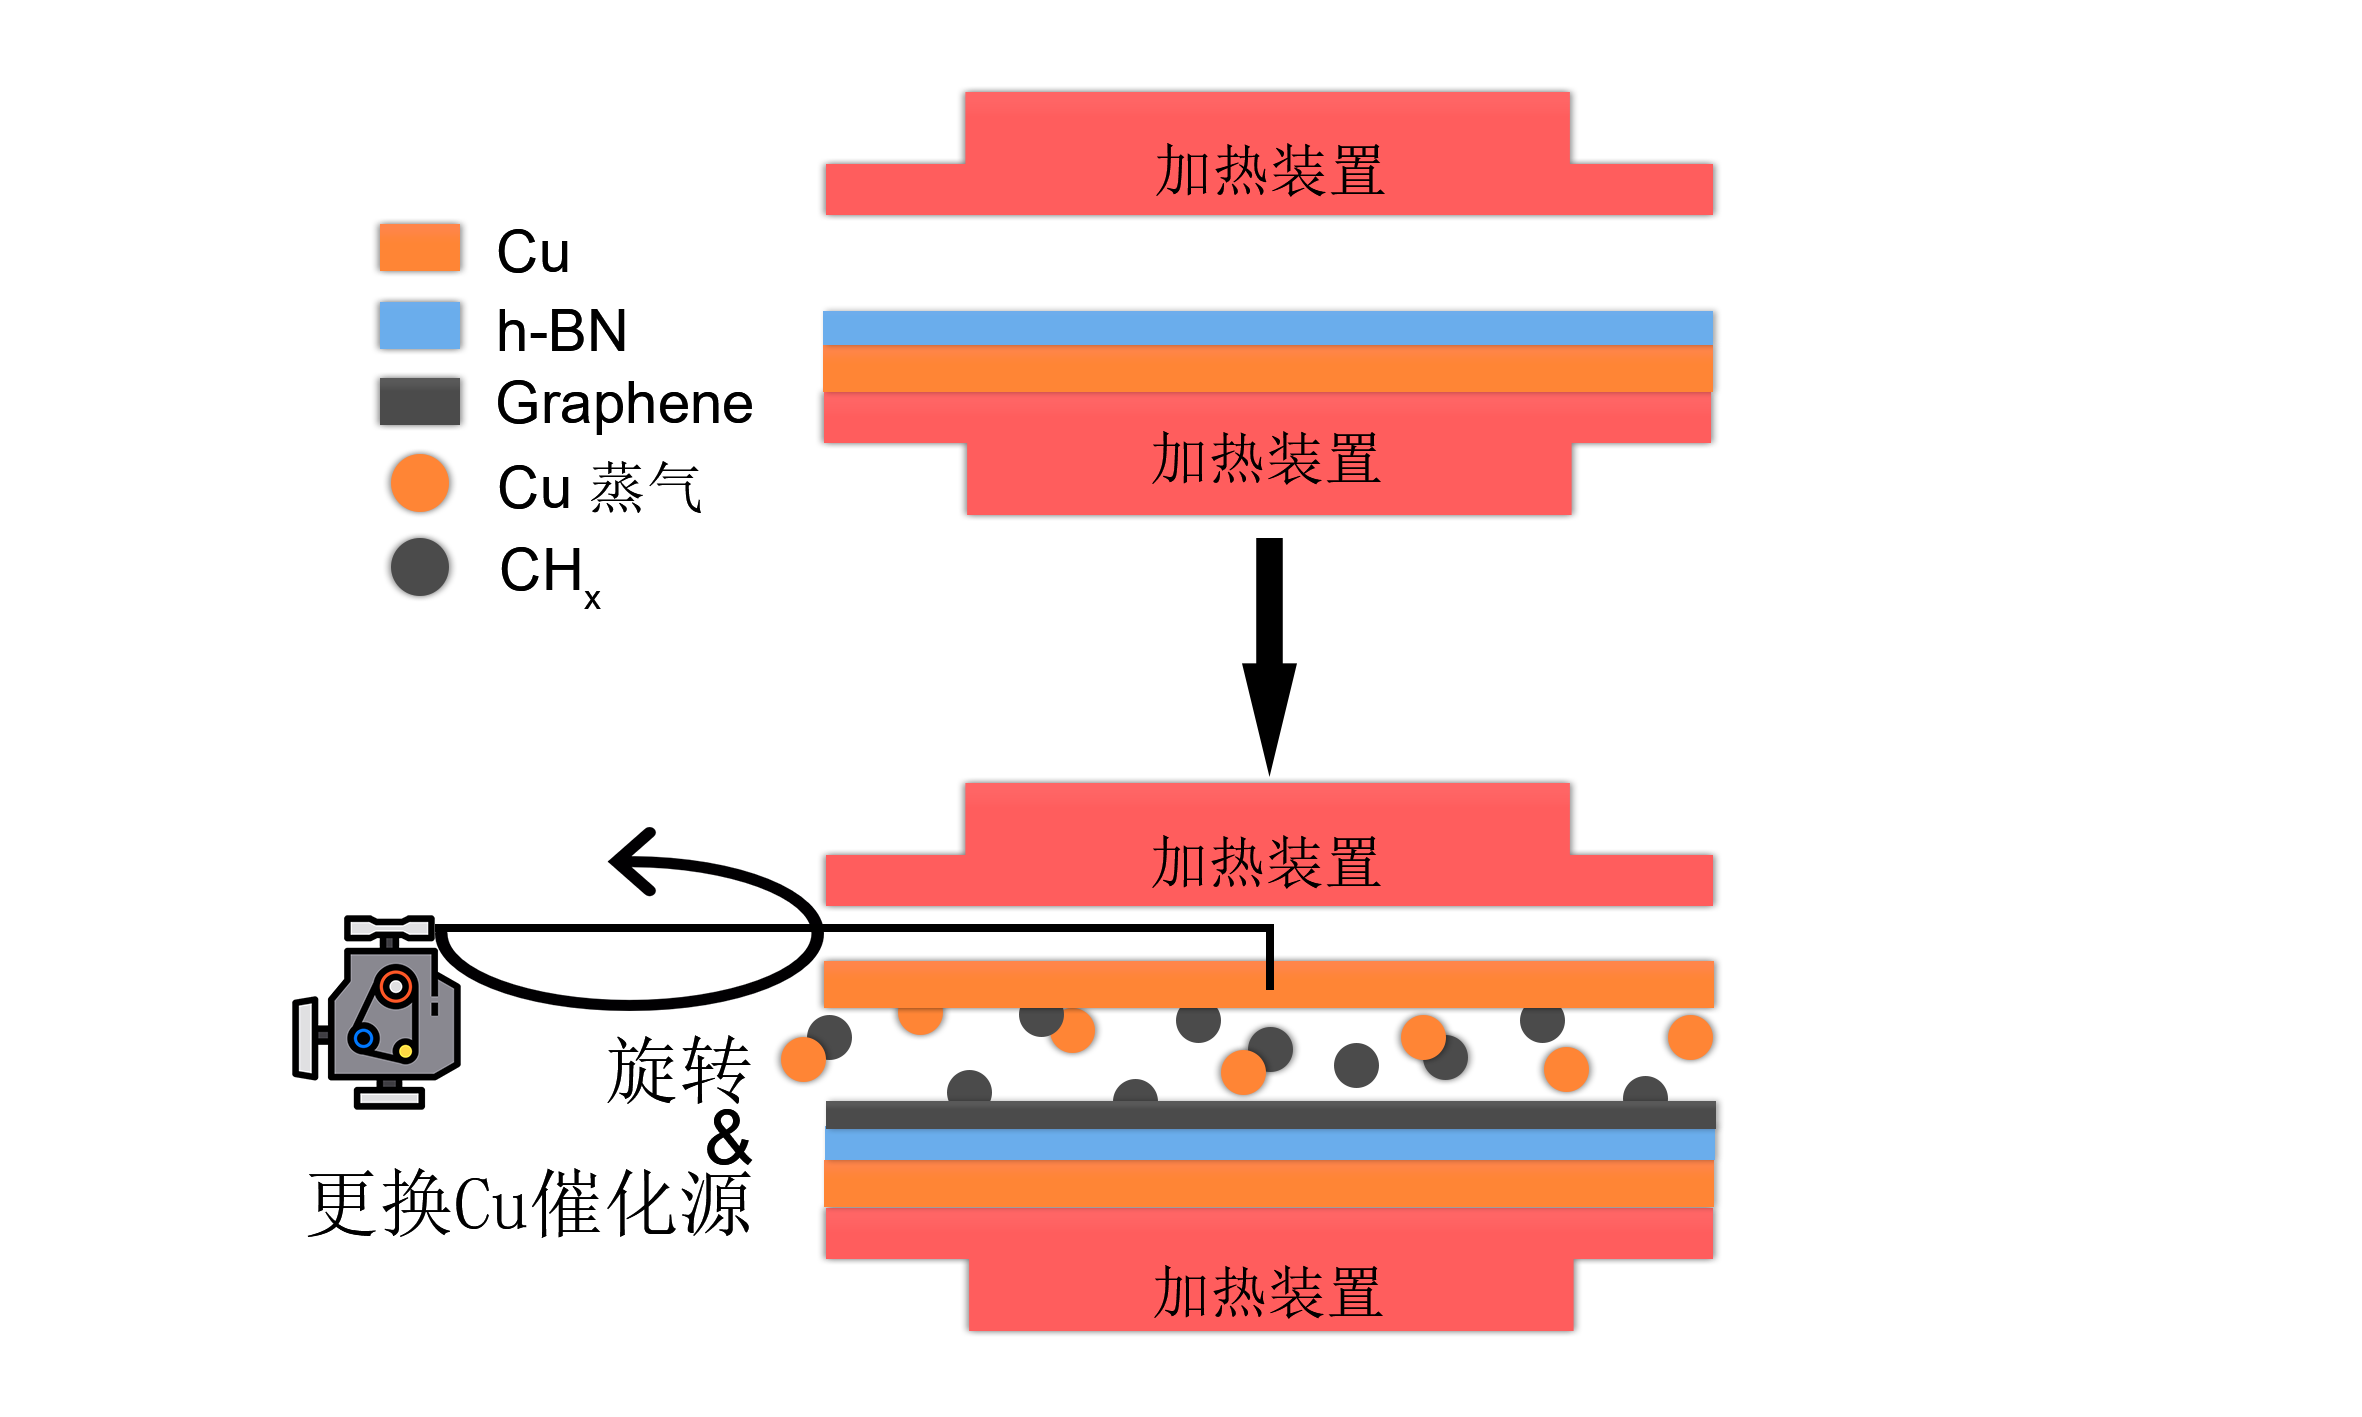
\includegraphics{pic/CG_diagram_routine.png}
            \label{fig:CG_diagram_routine}
        }\\[-0.5ex]
        \subfloat[]{
            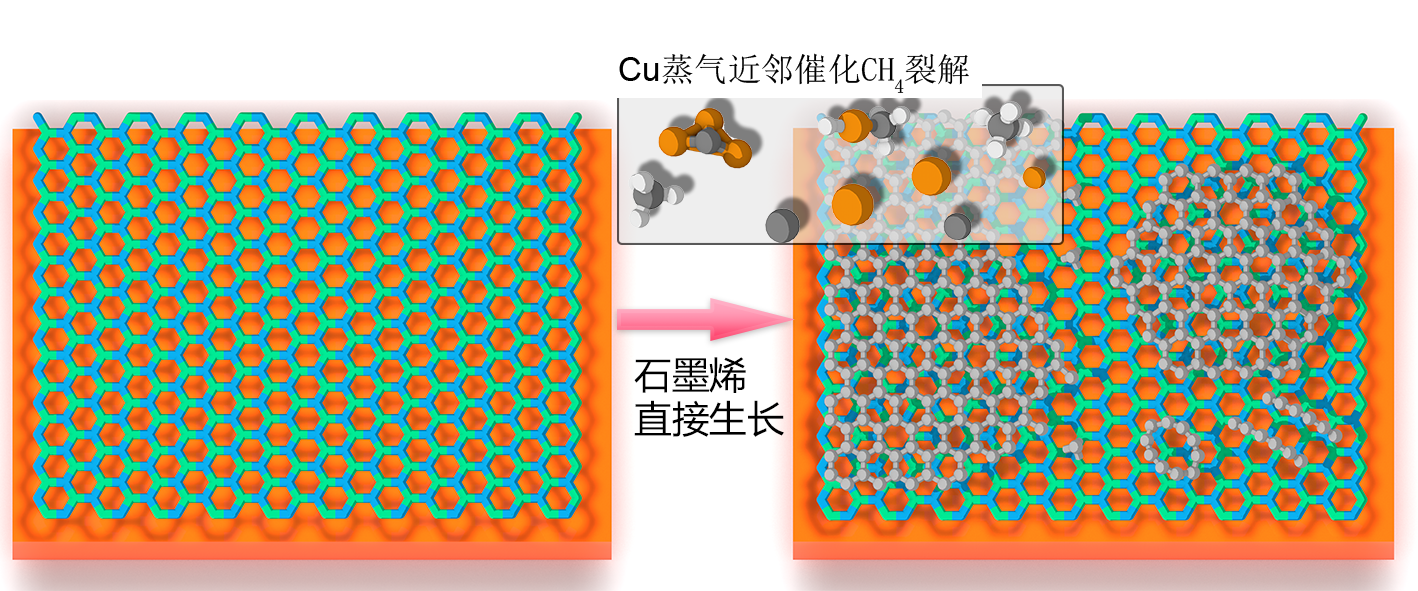
\includegraphics{pic/CG_diagram_growthSketch.png}
            \label{fig:CG_diagram_growthSketch}
        }
        \caption{利用\cemb{Cu}蒸气近邻催化效应在\cemb{h-BN}表面直接堆叠生长石墨烯。(a)生长装置示意图;(b)石墨烯/\cemb{h-BN}异质结生长过程示意图。}
        \label{fig:CG_diagram_CVD}
    \end{figure}

    图\ref{fig:CG_diagram_routine}和图\ref{fig:CG_diagram_growthSketch}为我们设计的利用\cemb{Cu}蒸气近邻催化效应在\cemb{h-BN}表面直接堆叠生长石墨烯的装置示意图和生长机理示意图。首先,我们可以在下方的\cemb{Cu}衬底表面利用常规的低压化学气相沉积法大面积的生长\cemb{h-BN}。这里我们使用液态环硼氮烷(borazine)作为生长前驱体。下方的加热器为\cemb{h-BN}大面积生长时提供合适的生长温度。当\cemb{h-BN}覆盖满下方\cemb{Cu}衬底的表面时,我们在上上方的加热器处引入第二片\cemb{Cu}源用于蒸发产生\cemb{Cu}蒸气。蒸发开始了额一段时间之后,\cemb{Cu}蒸气在扩散作用下充满\cemb{h-BN}上方的空间,此时引入甲烷\cemb{CH4}作为石墨烯生长的前驱体,通过调整\cemb{h-BN}和上方铜蒸发源之间的距离至合适的位置,我们就可以在下方\cemb{Cu}表面的已生长\cemb{h-BN}的表面直接堆叠生长石墨烯。需要注意的是,由于作为前驱体的甲烷\cemb{CH4}直接通入衬底和蒸发源之间的间隙,因此会在上方\cemb{Cu}蒸发源的表面形成石墨烯,当石墨烯覆盖满上方的\cemb{Cu}蒸发源的表面后,\cemb{Cu}蒸发源将会失去产生原有的\cemb{Cu}蒸气的能力,无法继续为\cemb{h-BN}表面甲烷的裂解提供气态催化剂。这时需要通过机械装置(图\ref{fig:CG_diagram_routine})替换掉已经蒸发能力衰减的\cemb{Cu}蒸发源,利用新换上的表面无石墨烯的\cemb{Cu}蒸发源继续提供\cemb{Cu}蒸气在\cemb{h-BN}表面生长石墨烯。

    \subsection{气态\cemb{Cu}催化剂的扩散}
    \label{CG:FEM_CuVapor}
    事实上,在\cemb{h-BN}上方的\cemb{Cu}蒸发源对于石墨烯在\cemb{h-BN}表面的直接石墨烯生长可能纯在两种作用\chinesecolon 一种是如上文所说的,\cemb{Cu}蒸发源的表面蒸发出浓度较高的\cemb{Cu}蒸气,这些\cemb{Cu}蒸气在扩散至\cemb{h-BN}表面仍然能够保持较高的浓度和分压。随后在\cemb{Cu}蒸气的催化作用下,生长气氛中的\cemb{CH4}逐渐脱氢裂解为活性碳原子\cemb{C},在\cemb{h-BN}表面成核生长成为石墨烯。另一种方式是\cemb{CH4}直接在\cemb{Cu}的表面脱氢裂解,产生的活性碳原子(\cemb{C})和活性碳氢化合物(\cemb{CH})等基团在热动能的作用下脱离\cemb{Cu}铜蒸发源的表面,扩散至下方\cemb{h-BN}的表面进行成核、生长石墨烯。

    \begin{figure}[htb]
        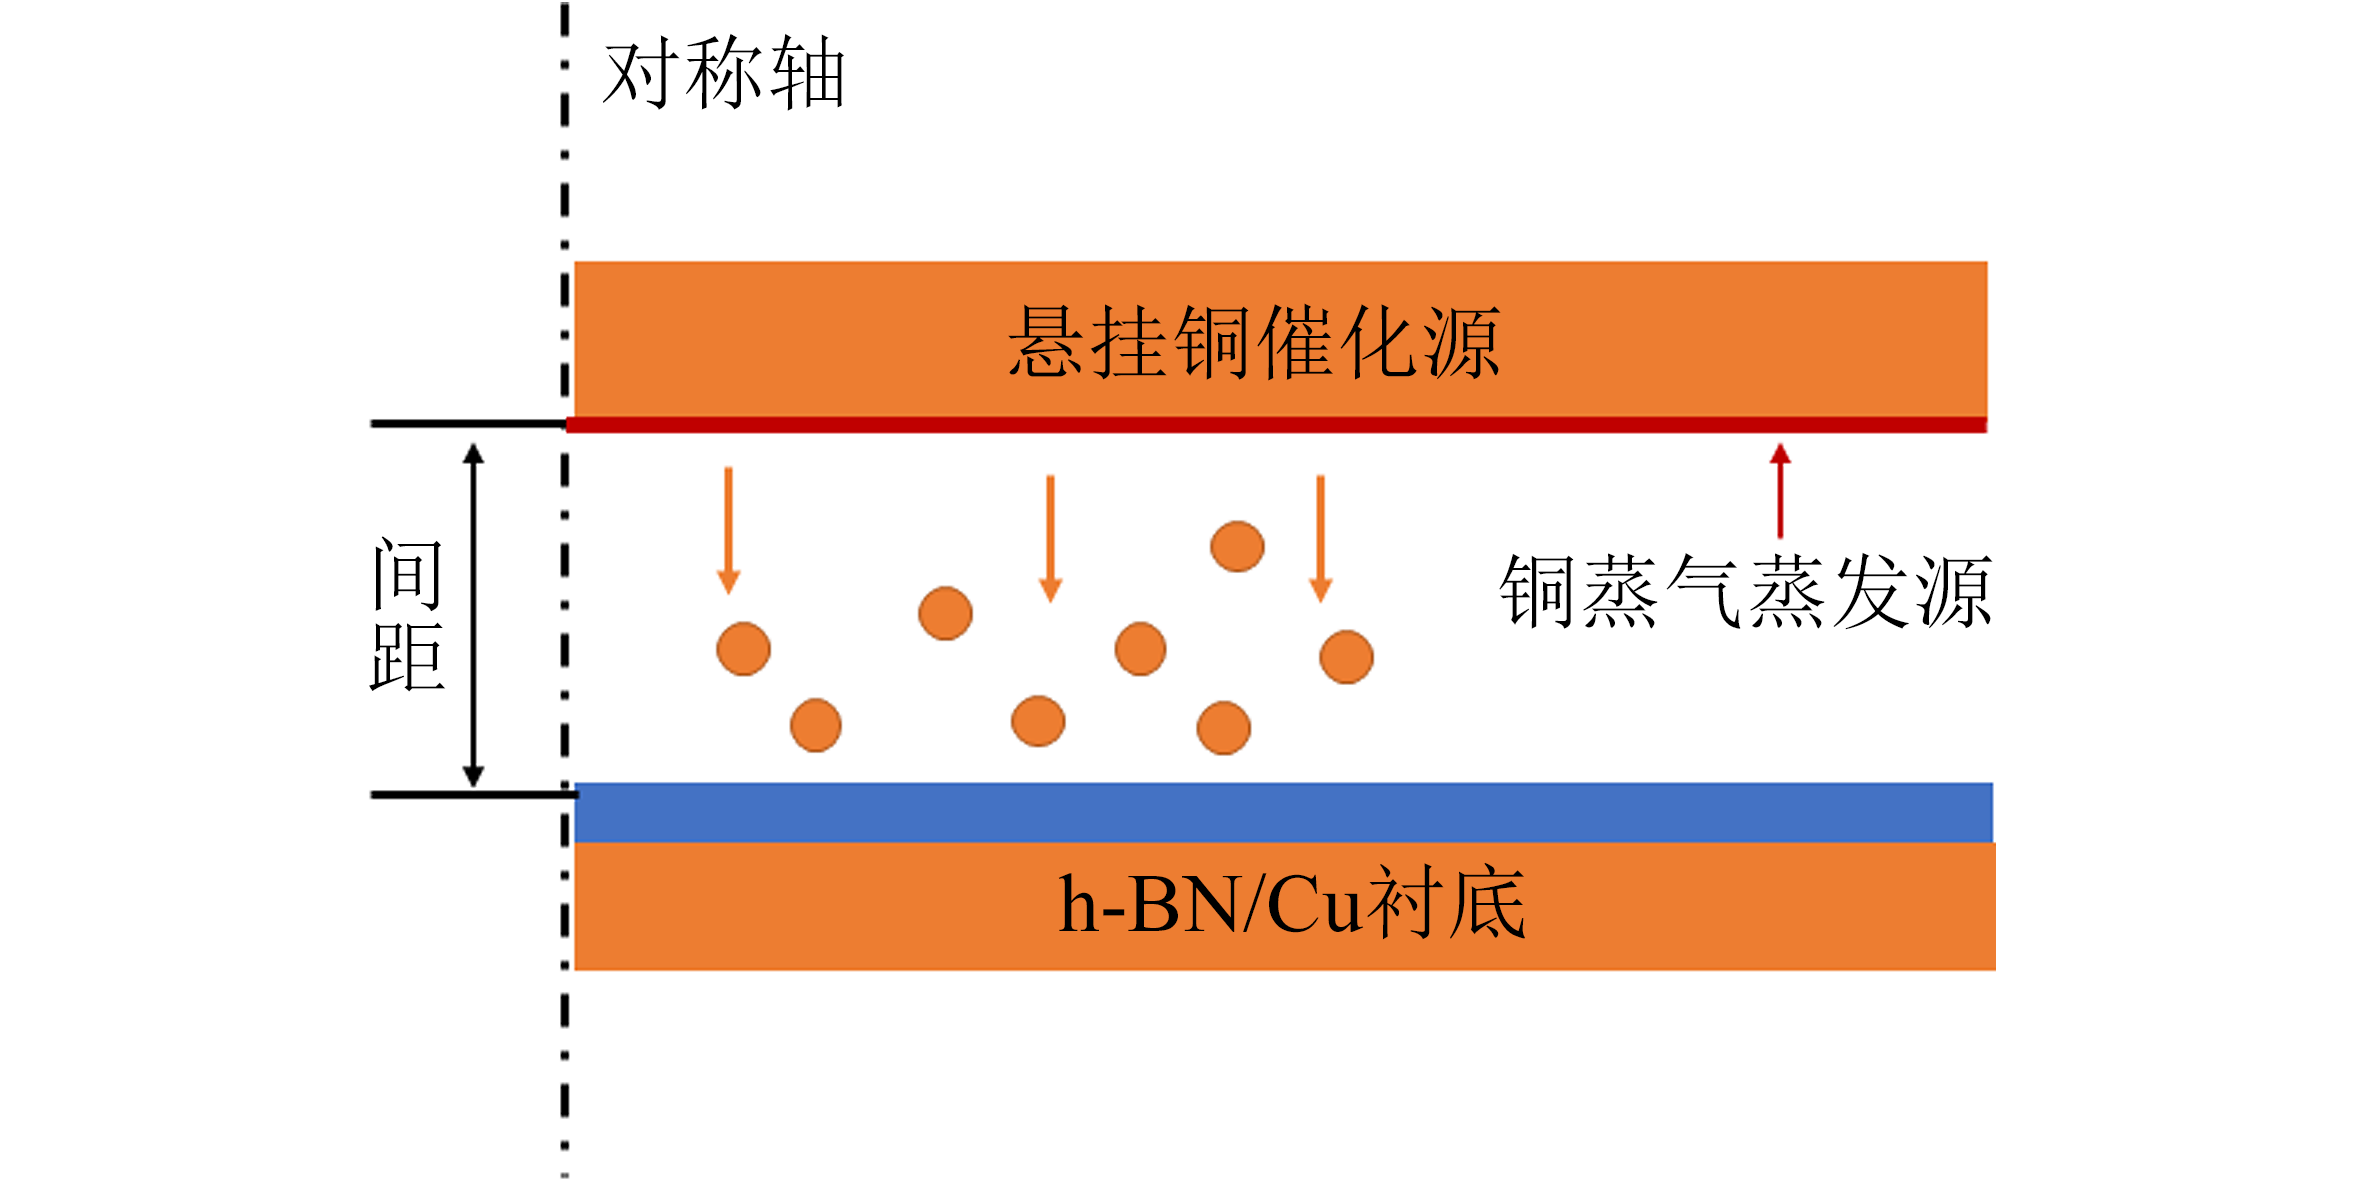
\includegraphics{pic/CG_diagram_FEM_structure.png}
        \caption{化学气相沉积腔体内\cemb{Cu}蒸气扩散模拟示意图。}
        \label{fig:CG_diagram_FEM_structure}
    \end{figure}

    为了判定并且验证在\cemb{h-BN}表面生长石墨烯的生长机制,我们首先使用自由分子流模拟\cemb{Cu}蒸发源产生的\cemb{Cu}蒸气在扩散至\cemb{h-BN}表面后的浓度。图\ref{fig:CG_diagram_FEM_structure}为我们所构建的在自由分子流模型下\cemb{Cu}蒸气产生和扩散的模拟结构图。我们考虑圆盘形的\cemb{Cu}衬底和\cemb{Cu}蒸发源,半径为\SI{500}{\micro\meter}。\cemb{Cu}蒸发源悬挂在\cemb{Cu}衬底和\cemb{h-BN}的上方,间隔一定距离。\cemb{Cu}蒸发源的温度设置为\SI{1200}{\kelvin},此时蒸发出的\cemb{Cu}蒸气的饱和蒸汽压约为\SI{1.25E-13}{\pascal}。对于蒸发出的\cemb{Cu}蒸气,我们只关注从蒸发源下表面蒸发出的\cemb{Cu}原子流,并且遵循朗缪尔蒸发公式(Langmuir’s Equation of evaporation)。
    
    \begin{figure}[htb]
        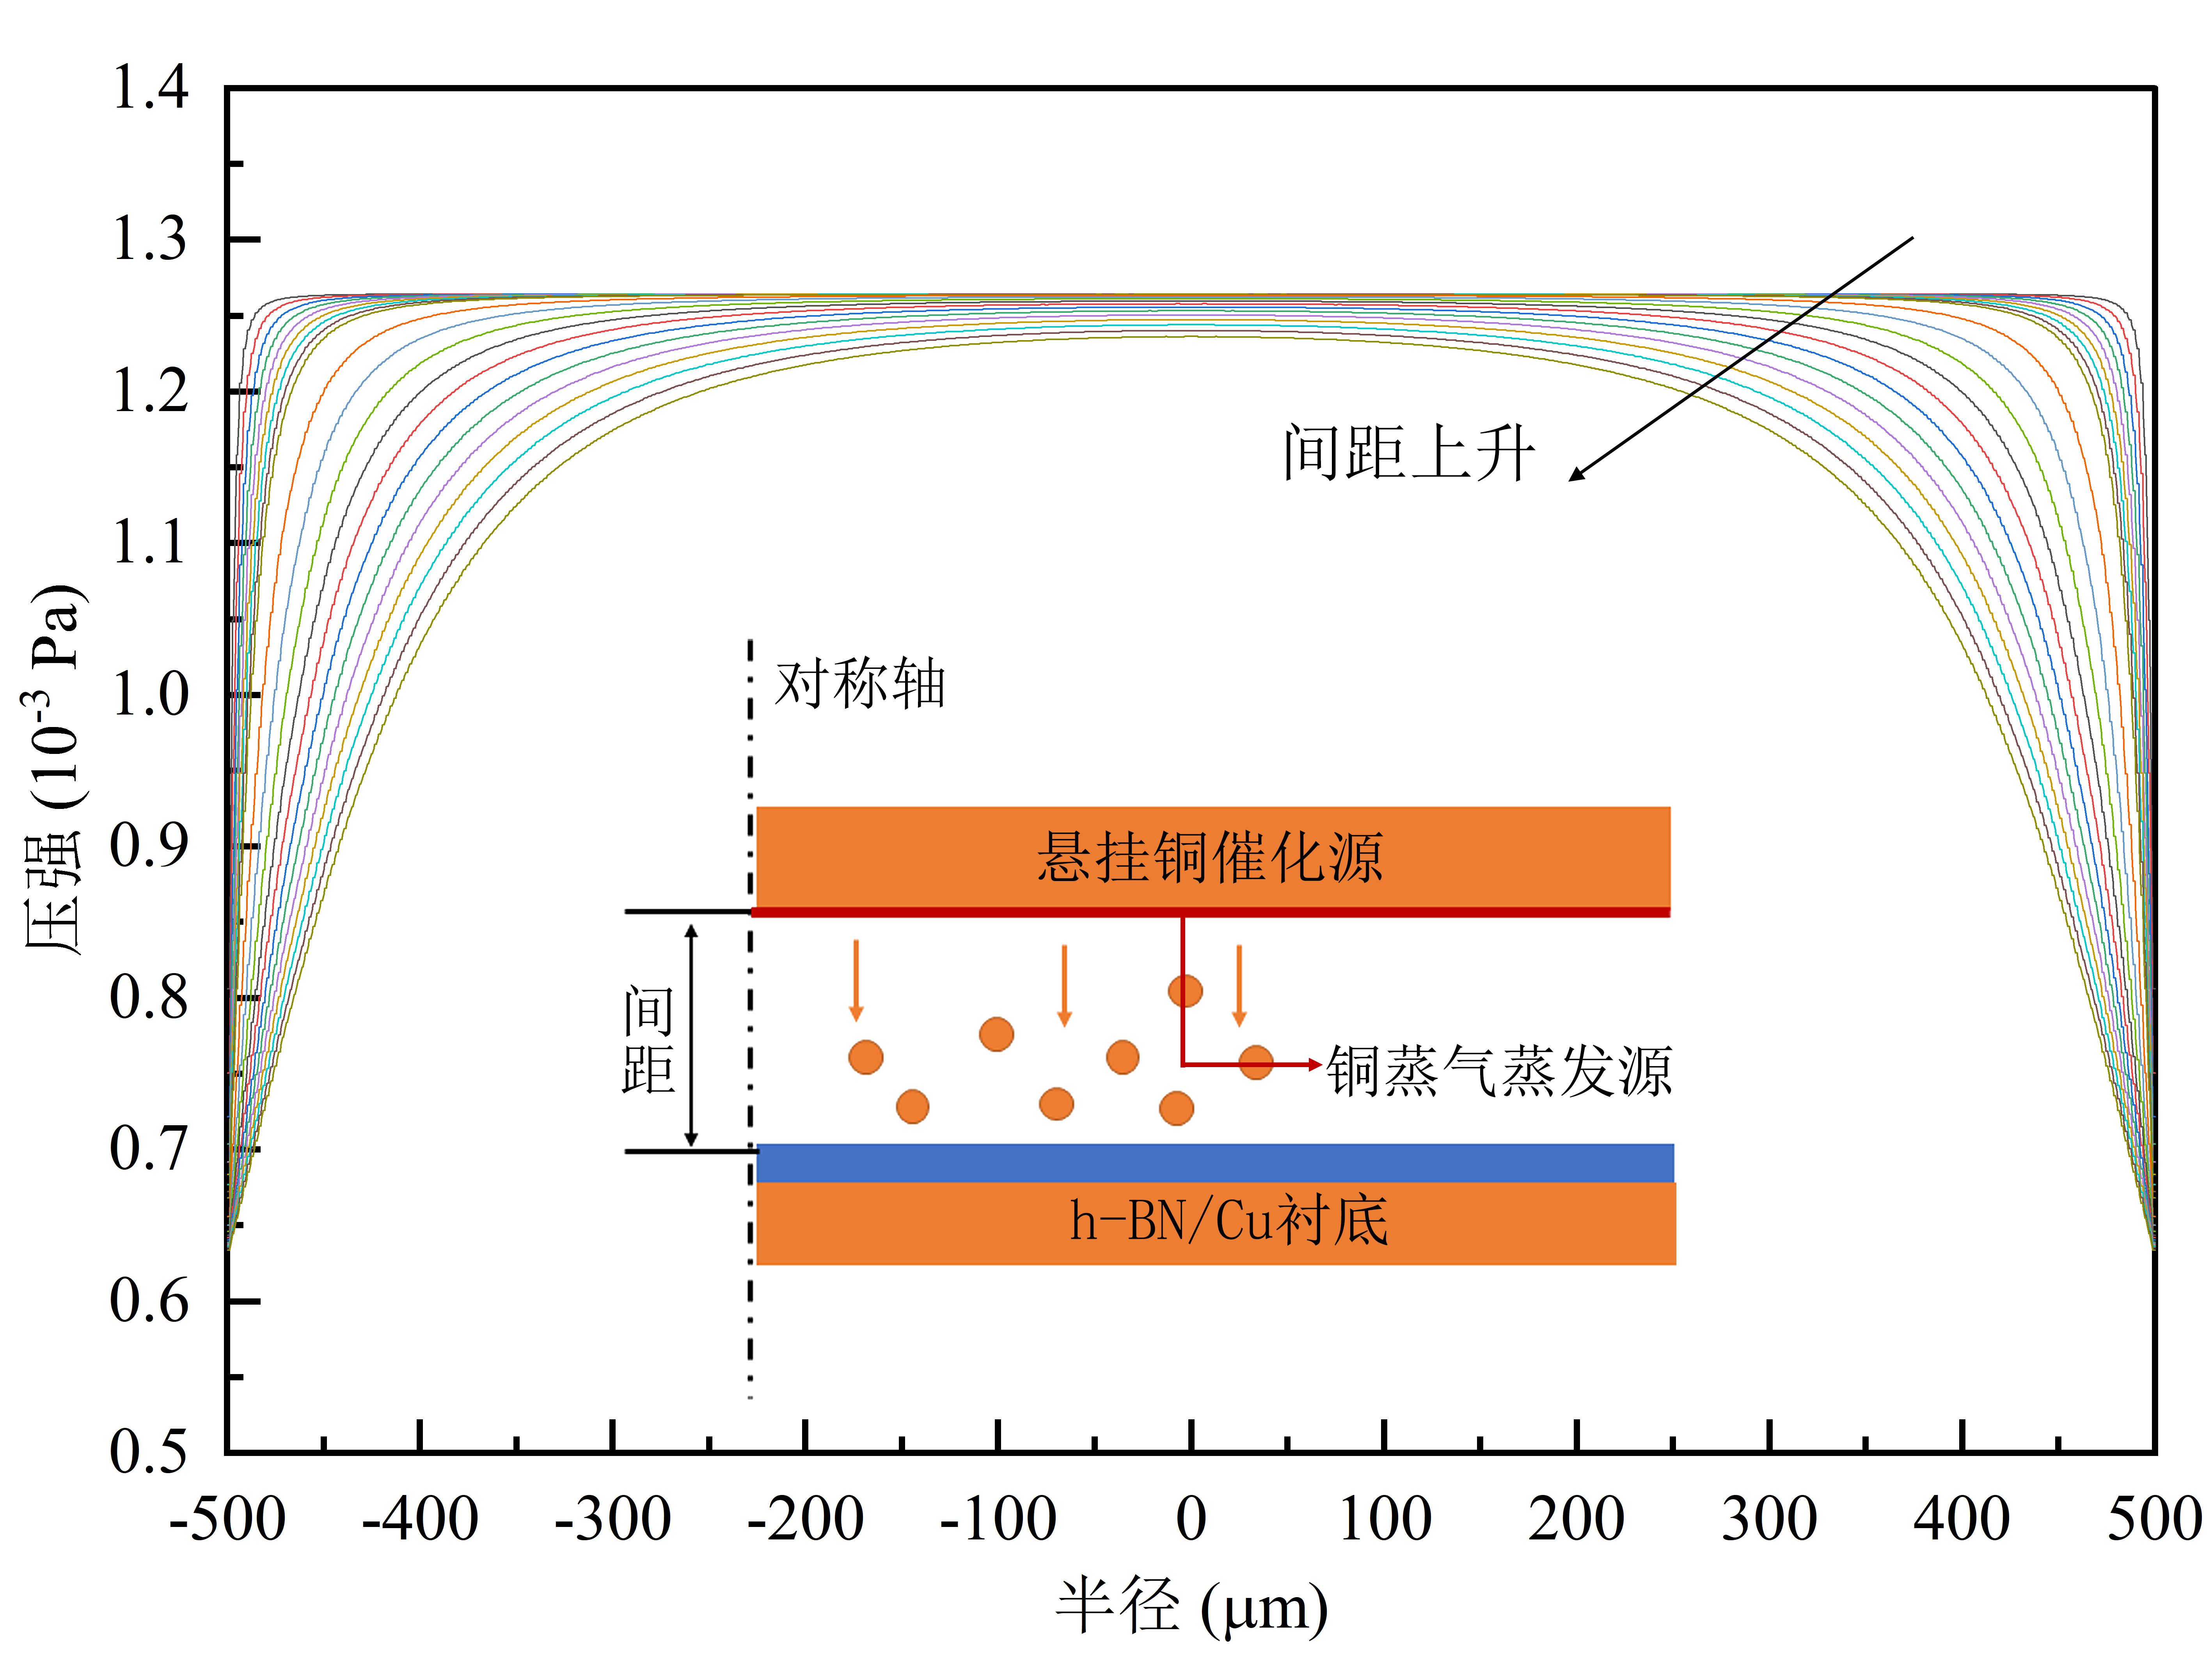
\includegraphics{pic/CG_FEM_fullCu.png}
        \caption{不同间距下\cemb{Cu/h-BN}表面\cemb{Cu}蒸气的气压分布情况。}
        \label{fig:CG_FEM_fullCu}
    \end{figure}

    使用自由分子流模拟,我们首先研究上方的\cemb{Cu}蒸发源未被石墨烯覆盖的情况。在图\ref{fig:CG_FEM_fullCu}中我们绘制了蒸发源和\cemb{Cu/h-BN}表面的距离在$\SI{4}{\micro\meter} \sim \SI{100}{\micro\meter}$的时候和,蒸发至下方\cemb{Cu/h-BN}表面的\cemb{Cu}蒸气的气压分布情况。可以看到对于\cemb{Cu/h-BN}表面,即使上方\cemb{Cu}蒸发源的距离从\SI{4}{\micro\meter}扩大至\SI{100}{\micro\meter}其的中心处的\cemb{Cu}蒸气的气压略微下降,接近于蒸发温度下的\cemb{Cu}原子的饱和蒸汽压\SI{1.25e-13}{\pascal}。当\cemb{Cu}蒸发源和\cemb{Cu/h-BN}之间的距离很近时,\cemb{Cu/h-BN}表面\cemb{Cu}蒸气的气压随着半径的衰减很小,只在接近边缘的位置由于\cemb{Cu}蒸气的向外扩散,导致\cemb{Cu/h-BN}表面边缘处(半径$\geqslant \SI{400}{\micro\meter}$)出现了\cemb{Cu}蒸气气压的明显下降。
    
    当\cemb{Cu}蒸发源和\cemb{Cu/h-BN}的距离扩大时,在\cemb{Cu/h-BN}表面\cemb{Cu}蒸气气压随着半径的衰减作用变强。当二者的距离提高到\SI{100}{\micro\meter}时,在\cemb{Cu/h-BN}表面半径为\SI{300}{\micro\meter}位置就已经可以观察到较为明显的\cemb{Cu}蒸气气压下降。当\cemb{Cu}蒸发源未被石墨烯覆盖的时候,在\cemb{Cu/h-BN}表面最外缘处(\SI{500}{\micro\meter})的\cemb{Cu}蒸气气压随与\cemb{Cu}蒸发源之间距离的上升而下降的驱使不明显。当距离为\SI{4}{\micro\meter}时,\cemb{Cu/h-BN}表面最外缘处的\cemb{Cu}蒸气气压为\SI{8e-4}{\pascal}。而当距离扩展到\SI{100}{\micro\meter}时,在\cemb{Cu/h-BN}表面最外缘处仍可以保持大约\SI{6e-4}{\pascal}的\cemb{Cu}蒸气。

    当在\cemb{Cu/h-BN}的表面生长了一段时间的石墨烯后,由于\cemb{CH4}在\cemb{Cu}蒸发源的表面同样会裂解沉积生长石墨烯,\cemb{Cu}蒸发源会有部分表面覆盖上新生长的石墨烯而从而失去蒸发\cemb{Cu}蒸气的能力。考虑到石墨烯生长前驱体\cemb{CH4}通常来自\cemb{Cu}蒸发源外部的气流,因此我们简单的将\cemb{Cu}蒸发源表面随着生长过程进行而生长的石墨烯限制在\cemb{Cu}蒸发源圆盘的外缘(半径$\geqslant \SI{250}{\micro\meter}$)。在图\ref{fig:CG_FEM_halfCu}中,我们模拟了在被石墨烯覆盖了外半圈\cemb{Cu}蒸发源的情况下,扩散至\cemb{Cu/h-BN}表面\cemb{Cu}蒸气的气压分布情况。可以看到相比于完整的\cemb{Cu}蒸发源,即使在\cemb{Cu}蒸发源和\cemb{Cu/h-BN}相距很近的情况下(\SI{4}{\micro\meter}),被石墨烯覆盖的\cemb{Cu}蒸发源只能在\cemb{Cu/h-BN}表面的正对于未被石墨烯覆盖的\cemb{Cu}蒸发源的位置维持较高压强的\cemb{Cu}铜蒸气(半径$\leqslant \SI{250}{\micro\meter}$)。
    同时,在这些正对于未被石墨烯覆盖的\cemb{Cu}蒸发源的位置,扩散至其上的\cemb{Cu}蒸气的浓度随着距离上升而下降的速度也略快于未被石墨烯覆盖时的情况。

    \begin{figure}[htb]
        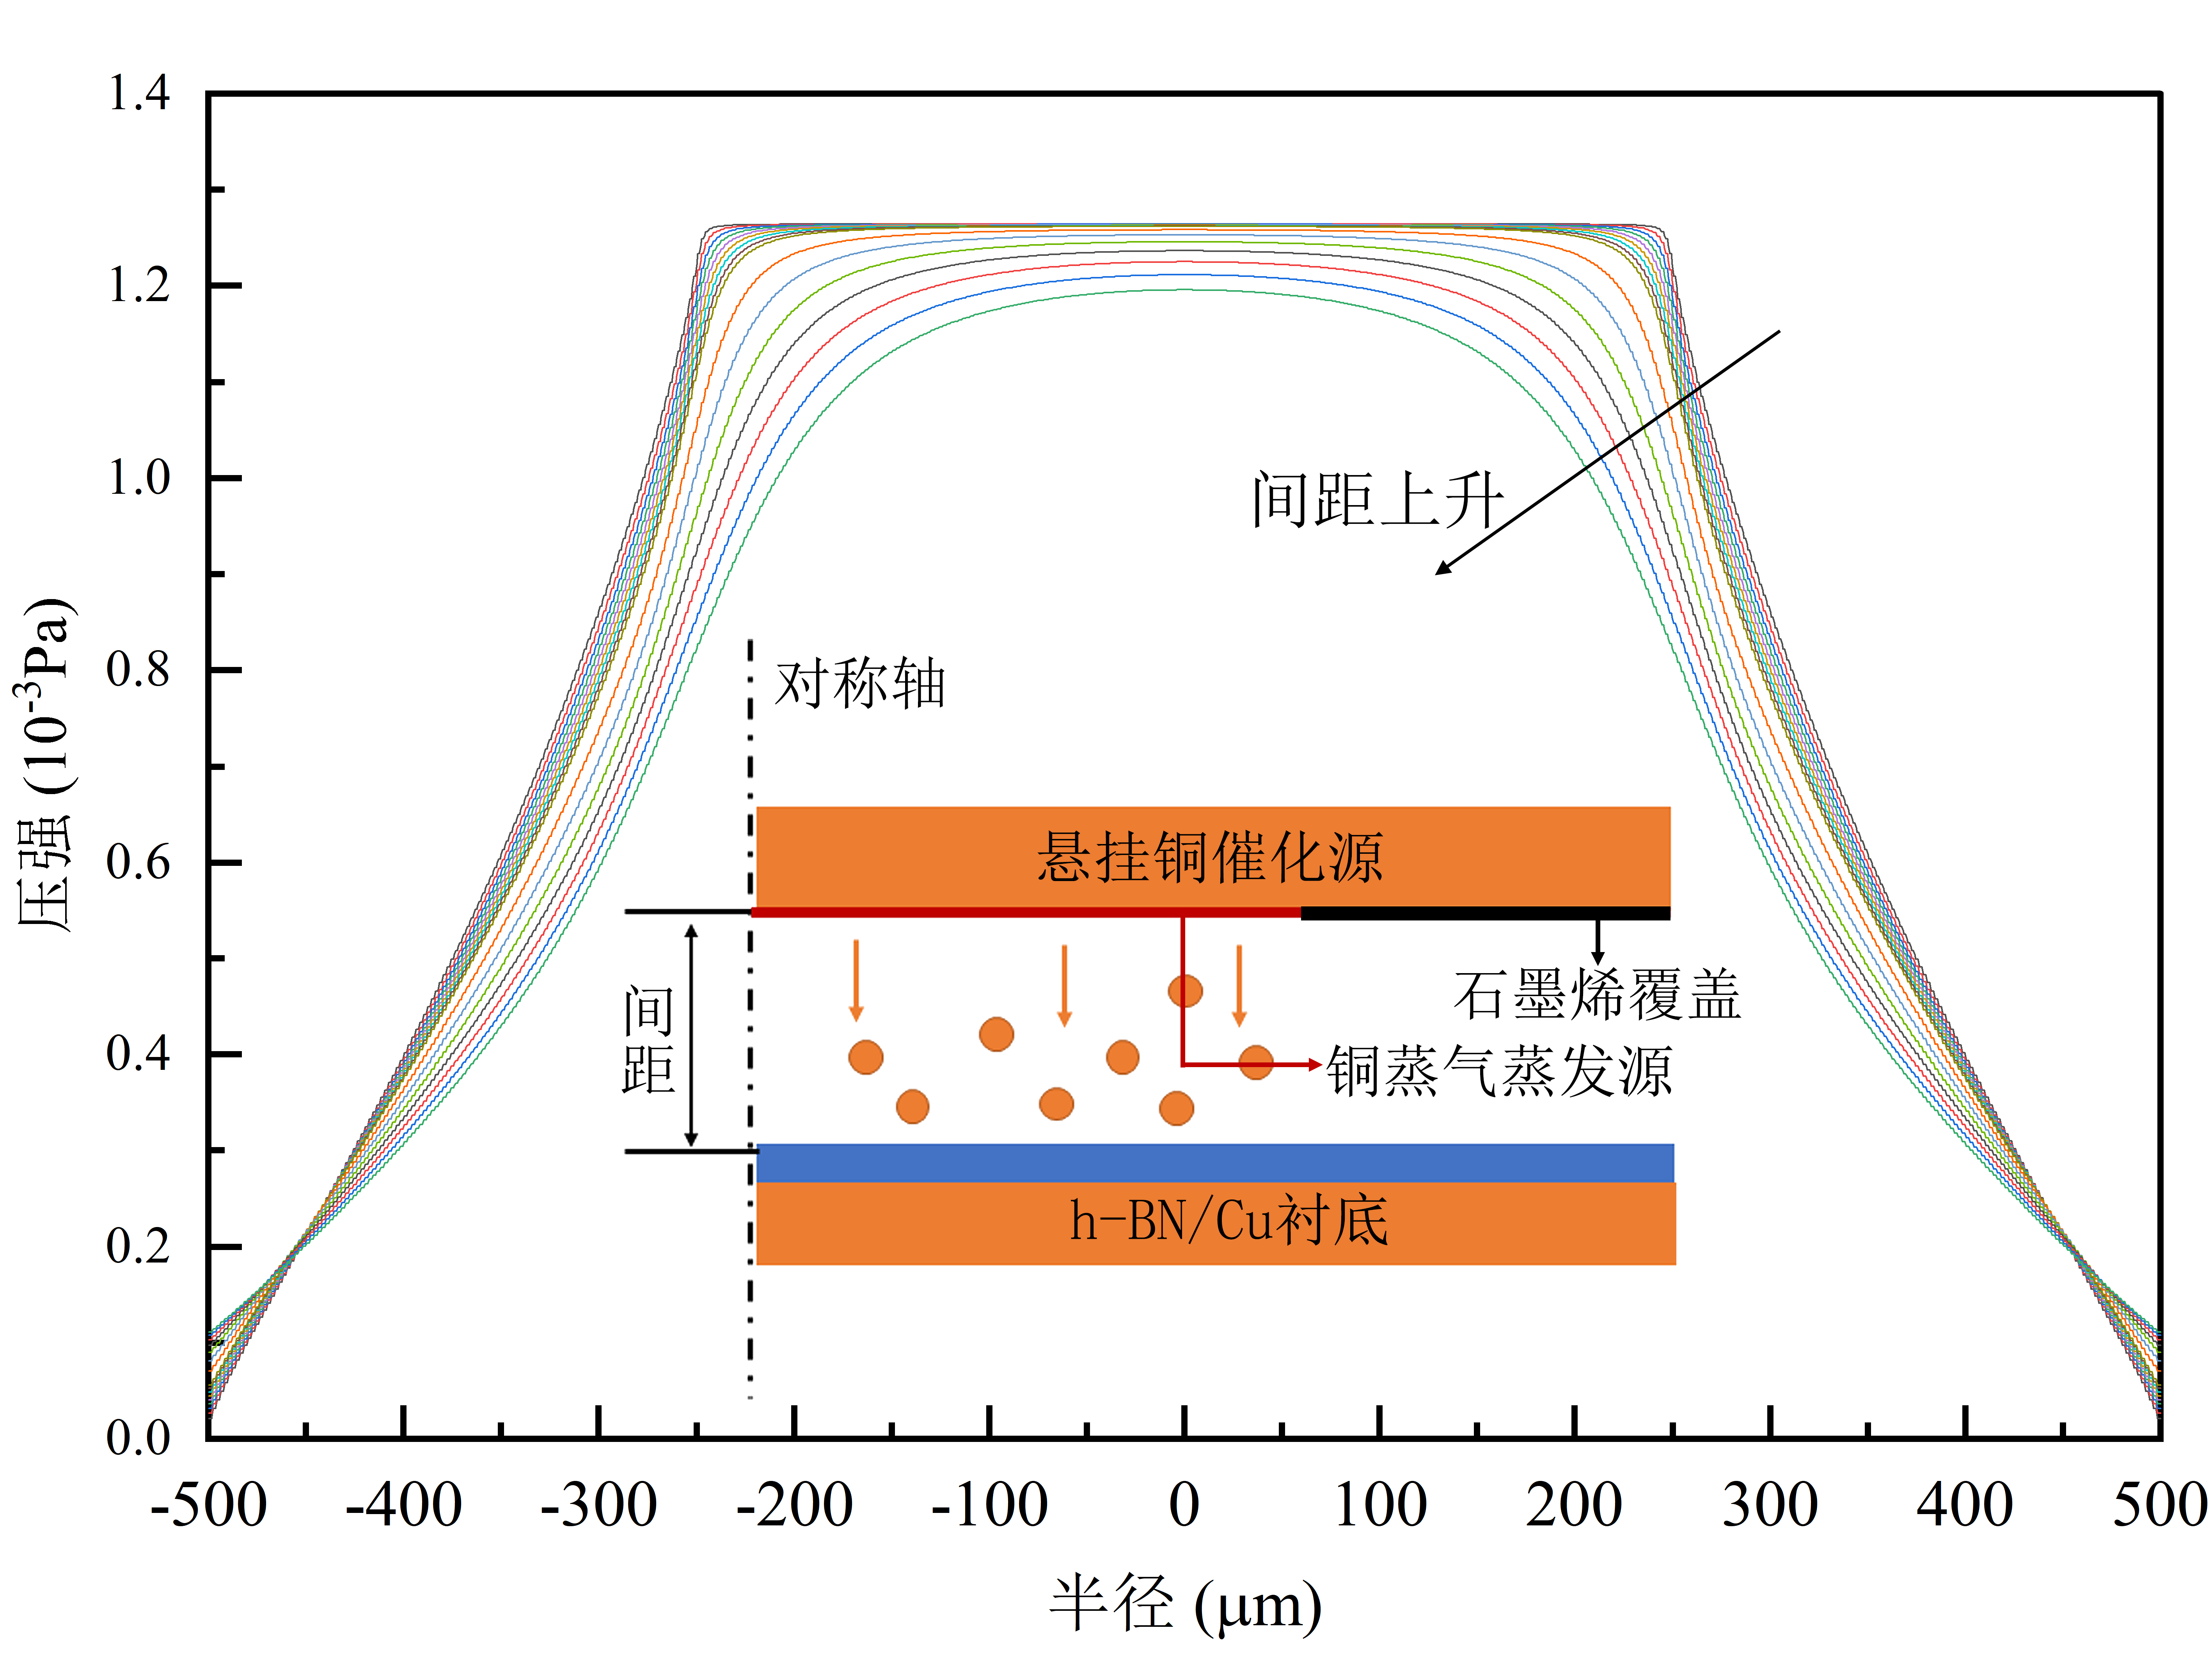
\includegraphics{pic/CG_FEM_halfCu.png}
        \caption{不同间距下\cemb{Cu}蒸发源的外半圈被石墨烯覆盖后蒸发、扩散至\cemb{Cu/h-BN}表面的\cemb{Cu}蒸气的气压分布情况。}
        \label{fig:CG_FEM_halfCu}
    \end{figure}

    而在\cemb{Cu/h-BN}表面正对于上方被石墨烯覆盖的\cemb{Cu}蒸发源的位置,扩散至这些位置的\cemb{Cu}蒸气的浓度急剧下降。在模拟系统中\cemb{Cu/h-BN}表面的边缘(\SI{500}{\micro\meter}),\cemb{Cu}蒸气的浓度下降至约\SI{1e-4}{\pascal},远低于未被石墨烯覆盖时的\SI{6E-4}{\pascal}。值得注意的是,在\cemb{Cu/h-BN}边缘的位置,\cemb{Cu}蒸发源和\cemb{Cu/h-BN}距离较远时\cemb{Cu}蒸气的浓度反超了距离较近时的情况(半径$\geqslant \SI{450}{\micro\meter}$)。这是由于在与\cemb{Cu}蒸发源的距离较远时,\cemb{Cu/h-BN}表面边缘能够更好的接收到来自\cemb{Cu}蒸发源中央的\cemb{Cu}蒸气原子,而这些原子在距离较近时会直接扩散至\cemb{Cu/h-BN}表面中央的区域。
    因此,悬挂的\cemb{Cu}蒸发源需要在生长过程中经常性得进行更换,以保持较为完整的\cemb{Cu}表面,防止石墨烯覆盖后对\cemb{Cu}蒸气扩散至下方\cemb{Cu/h-BN}表面的\cemb{Cu}蒸气的浓度和均匀度产生影响,最终导致在\cemb{Cu/h-BN}表面石墨烯生长速度减慢以及生长均匀性变差的情况。

    考虑到在实际的生长过程中,用于提供\cemb{Cu}蒸气的\cemb{Cu}蒸发源可以比生长区域大得多(尺寸在\si{\centi\meter}级),因此我们可以利用模拟\cemb{Cu/h-BN}中心处的\cemb{Cu}蒸气气压来代表生长区域中参与近邻催化裂解\cemb{CH4}的\cemb{Cu}蒸气气压。在图\ref{fig:CG_FEM_fullCuCenterVariousDistance}中,我们计算了\cemb{Cu}蒸发源和\cemb{Cu/h-BN}距离从微米级\si{\micro\meter}扩大至厘米级\si{\milli\meter}时,在石墨烯生长区域中\cemb{Cu}蒸气的气压变化情况。我们可以看到当距离小于\SI{1}{\milli\meter}(\SI{1000}{\micro\meter})时,从\cemb{Cu}蒸发源蒸发、扩散至\cemb{Cu/h-BN}表面的\cemb{Cu}蒸气的气压变化较小,且非常接近于\cemb{Cu}原子的饱和蒸汽压\SI{1.25e-13}{\pascal}。而当二者之间的距离继续增大,\cemb{Cu}蒸气的压强极速下降。距离为\SI{10}{\milli\meter}(\SI{10000}{\micro\meter})时,模拟得到的在\cemb{Cu/h-BN}表面的\cemb{Cu}蒸气的气压仅有约\SI{4e-4}{\pascal}。\cemb{Cu/h-BN}表面的\cemb{Cu}蒸气气压随距离的变化与实验中的现象一致。
    %TODO 引用
    随着\cemb{Cu}蒸发源和\cemb{Cu/h-BN}表面之间的距离由\SI{10}{\micro\meter}增长至\SI{1}{\milli\meter}和\SI{10}{\milli\meter},在\cemb{Cu/h-BN}表面直接生长的石墨烯的覆盖率也随之减少。

    \begin{figure}[htb]
        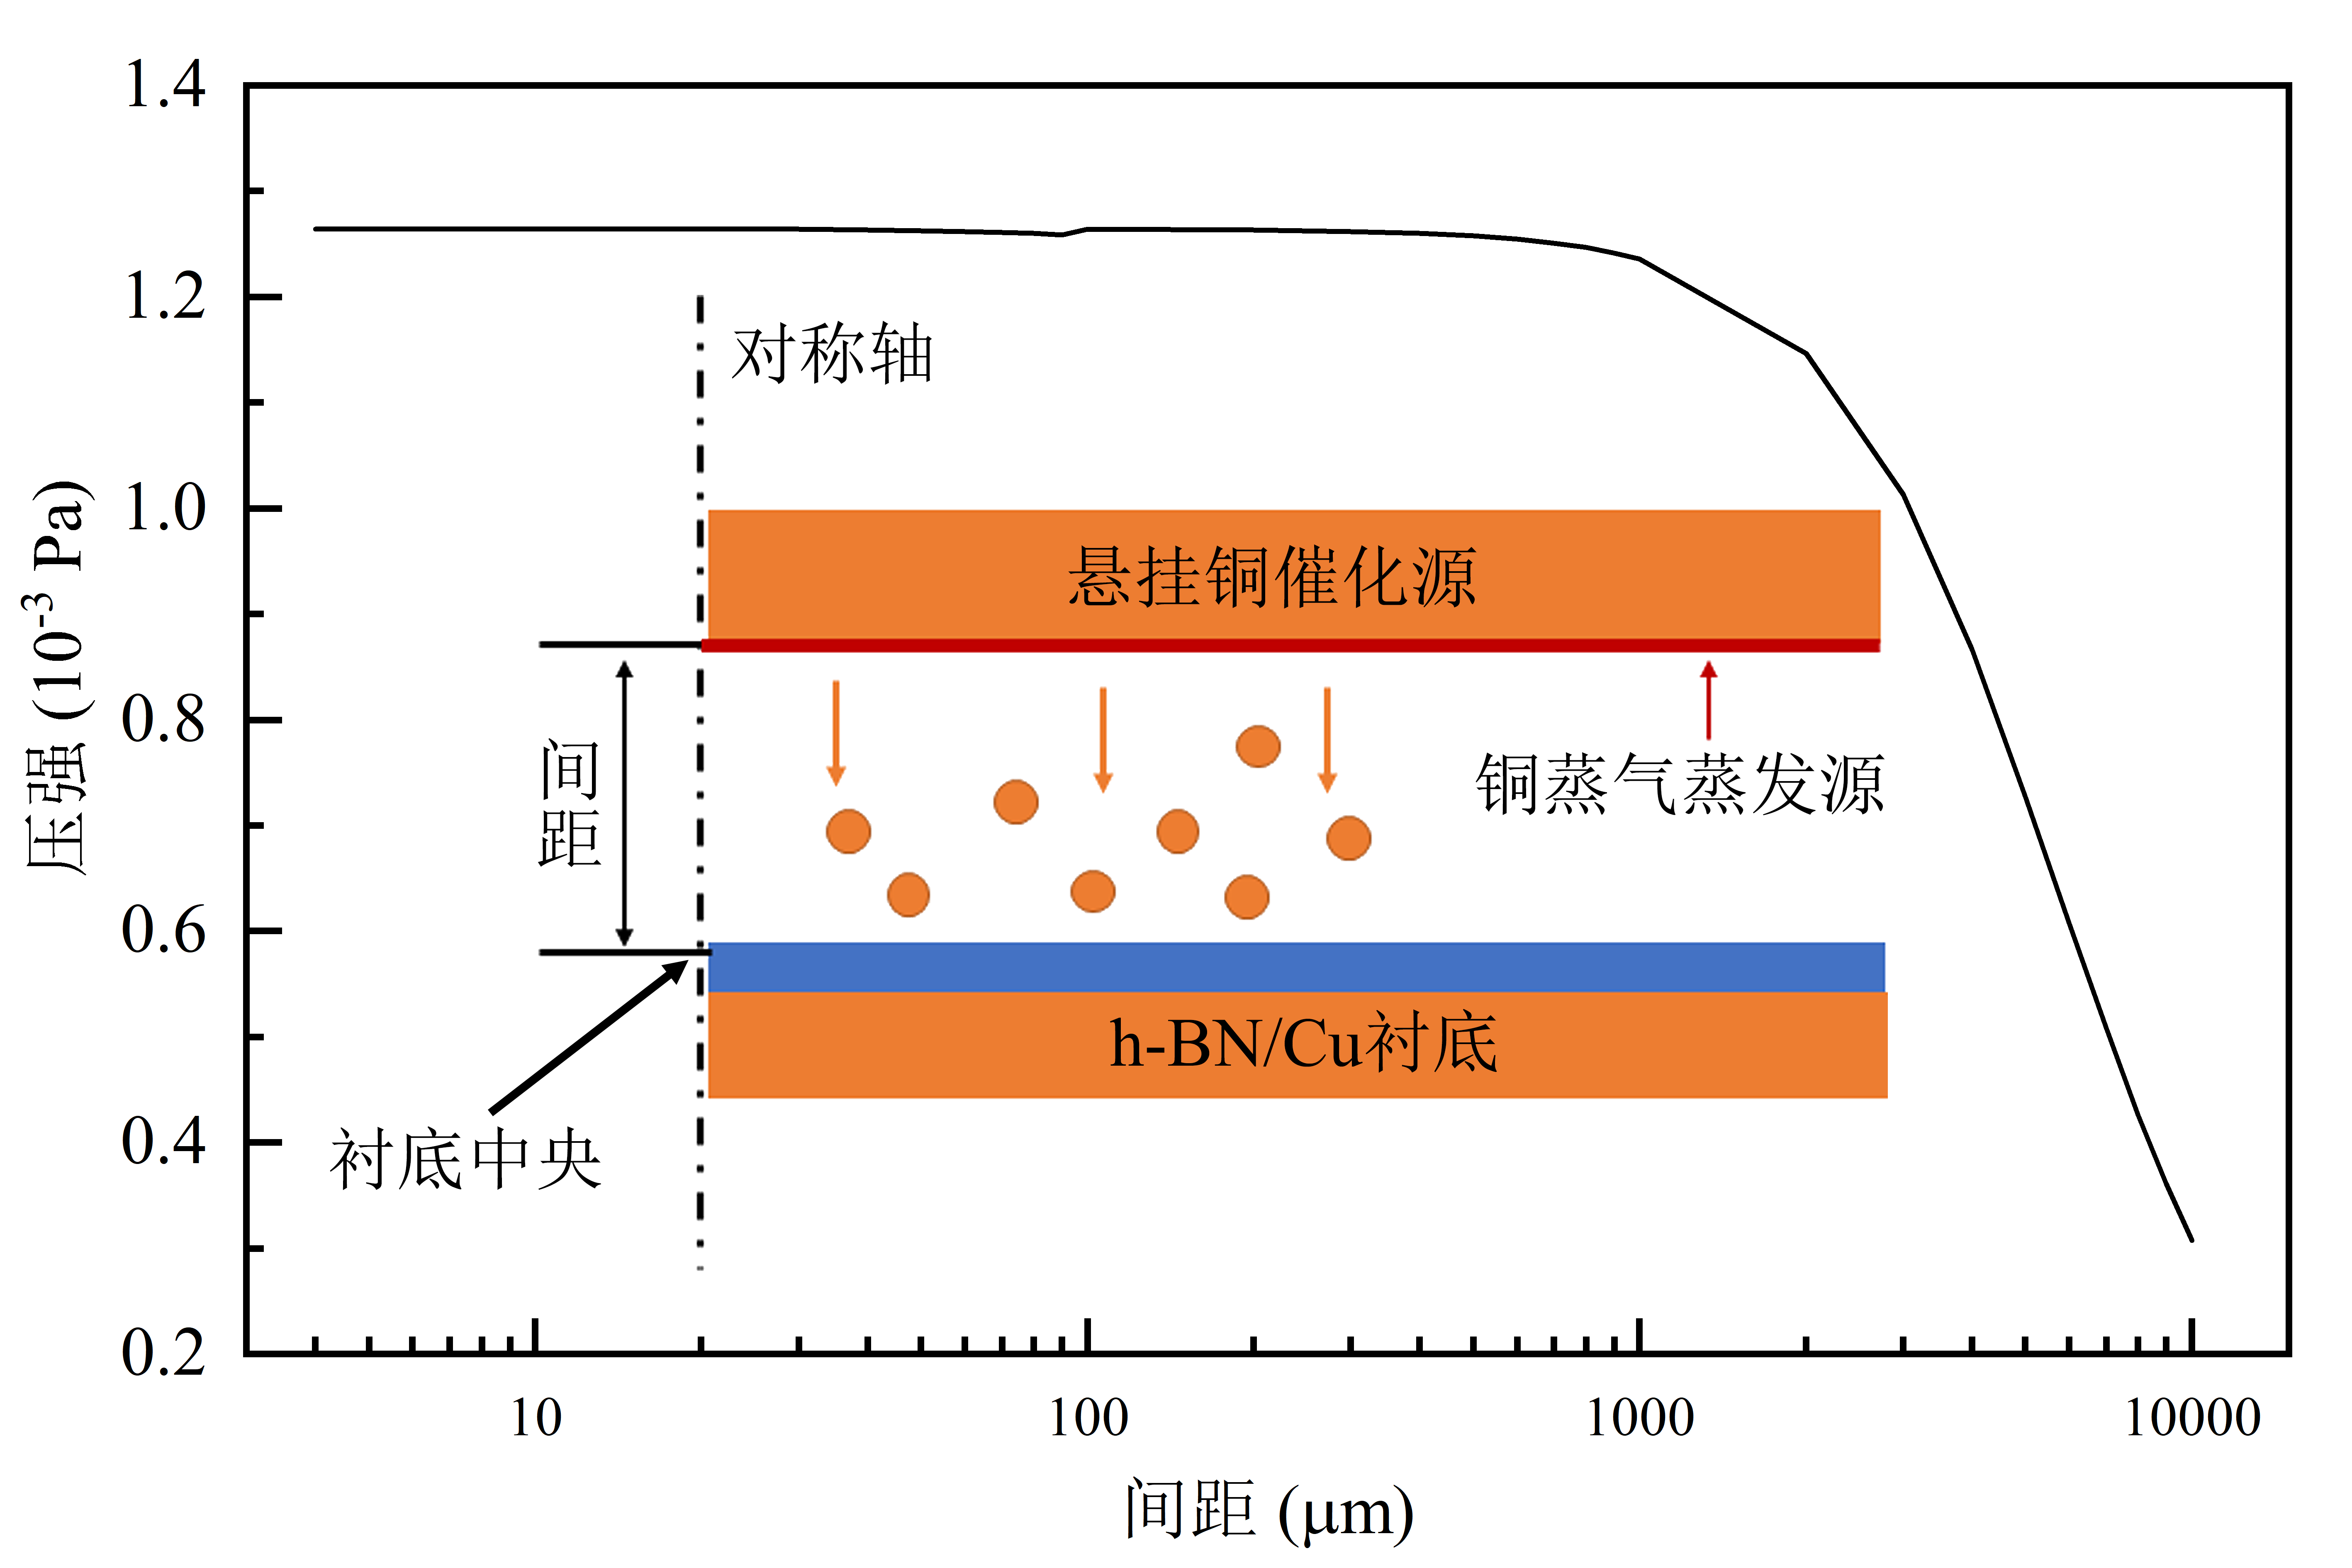
\includegraphics{pic/CG_FEM_fullCuCenterVariousDistance.png}
        \caption{不同间距下从\cemb{Cu}蒸发源蒸发、扩散至\cemb{Cu/h-BN}表面中央的\cemb{Cu}蒸气的气压情况。}
        \label{fig:CG_FEM_fullCuCenterVariousDistance}
    \end{figure}

    另一方面,考虑到在温度为\SI{1300}{\kelvin}时,石墨碳的饱和蒸汽压仅有\SI{1e-17}{\pascal}\citing{RN788-2004}。因此我们认为相比于从扩散而来的\cemb{C}、\cemb{CH},在\cemb{Cu/h-BN}表面直接堆叠生长的石墨烯更可能来源于前驱体\cemb{CH4}利用\cemb{Cu}蒸气的近邻催化作用在\cemb{Cu/h-BN}表面裂解而产生的\cemb{C}、\cemb{CH}等活性碳化物。

    \subsection{气态\cemb{Cu}催化剂对甲烷裂解反应的催化性能}
    在\ref{CG:FEM_CuVapor}章中,我们证明了当\cemb{Cu}蒸发源和\cemb{Cu/h-BN}衬底的距离足够近时,能够有足够的\cemb{Cu}蒸气扩散至\cemb{h-BN}的表面进行\cemb{CH4}裂解的催化作用。接下来我们利用密度泛函理论计算,探究\cemb{Cu}蒸气对于\cemb{CH4}脱氢裂解反应的催化作用。在计算中,我们使用包含$1\sim 3$个原子的\cemb{Cu}团簇(\cemb{Cu}、\cemb{Cu2}、\cemb{Cu3})代表\cemb{Cu}蒸气中的气态物质。\cemb{Cu}蒸气对于\cemb{CH4}裂解反应的催化能力通过考察\cemb{CH4}在不同\cemb{Cu}团簇表面的脱氢反应的激活能进行标定。在本章的激活能计算中,我们考虑\cemb{CH4}脱氢的四步脱氢基元反应,每步反应都从吸附在\cemb{Cu}团簇上的\cemb{CH4}分子中脱出一个\cemb{H}原子\chinesecolon
    \begin{equation}
        \label{chemeq:CH4deH}
        \begin{split}
            \cemb{CH4 &-> CH3 + H}\\
            \cemb{CH3 &-> CH2 + H}\\
            \cemb{CH2 &-> CH + H}\\
            \cemb{CH &-> C + H}
        \end{split}
    \end{equation}

    \begin{figure}[htb]
        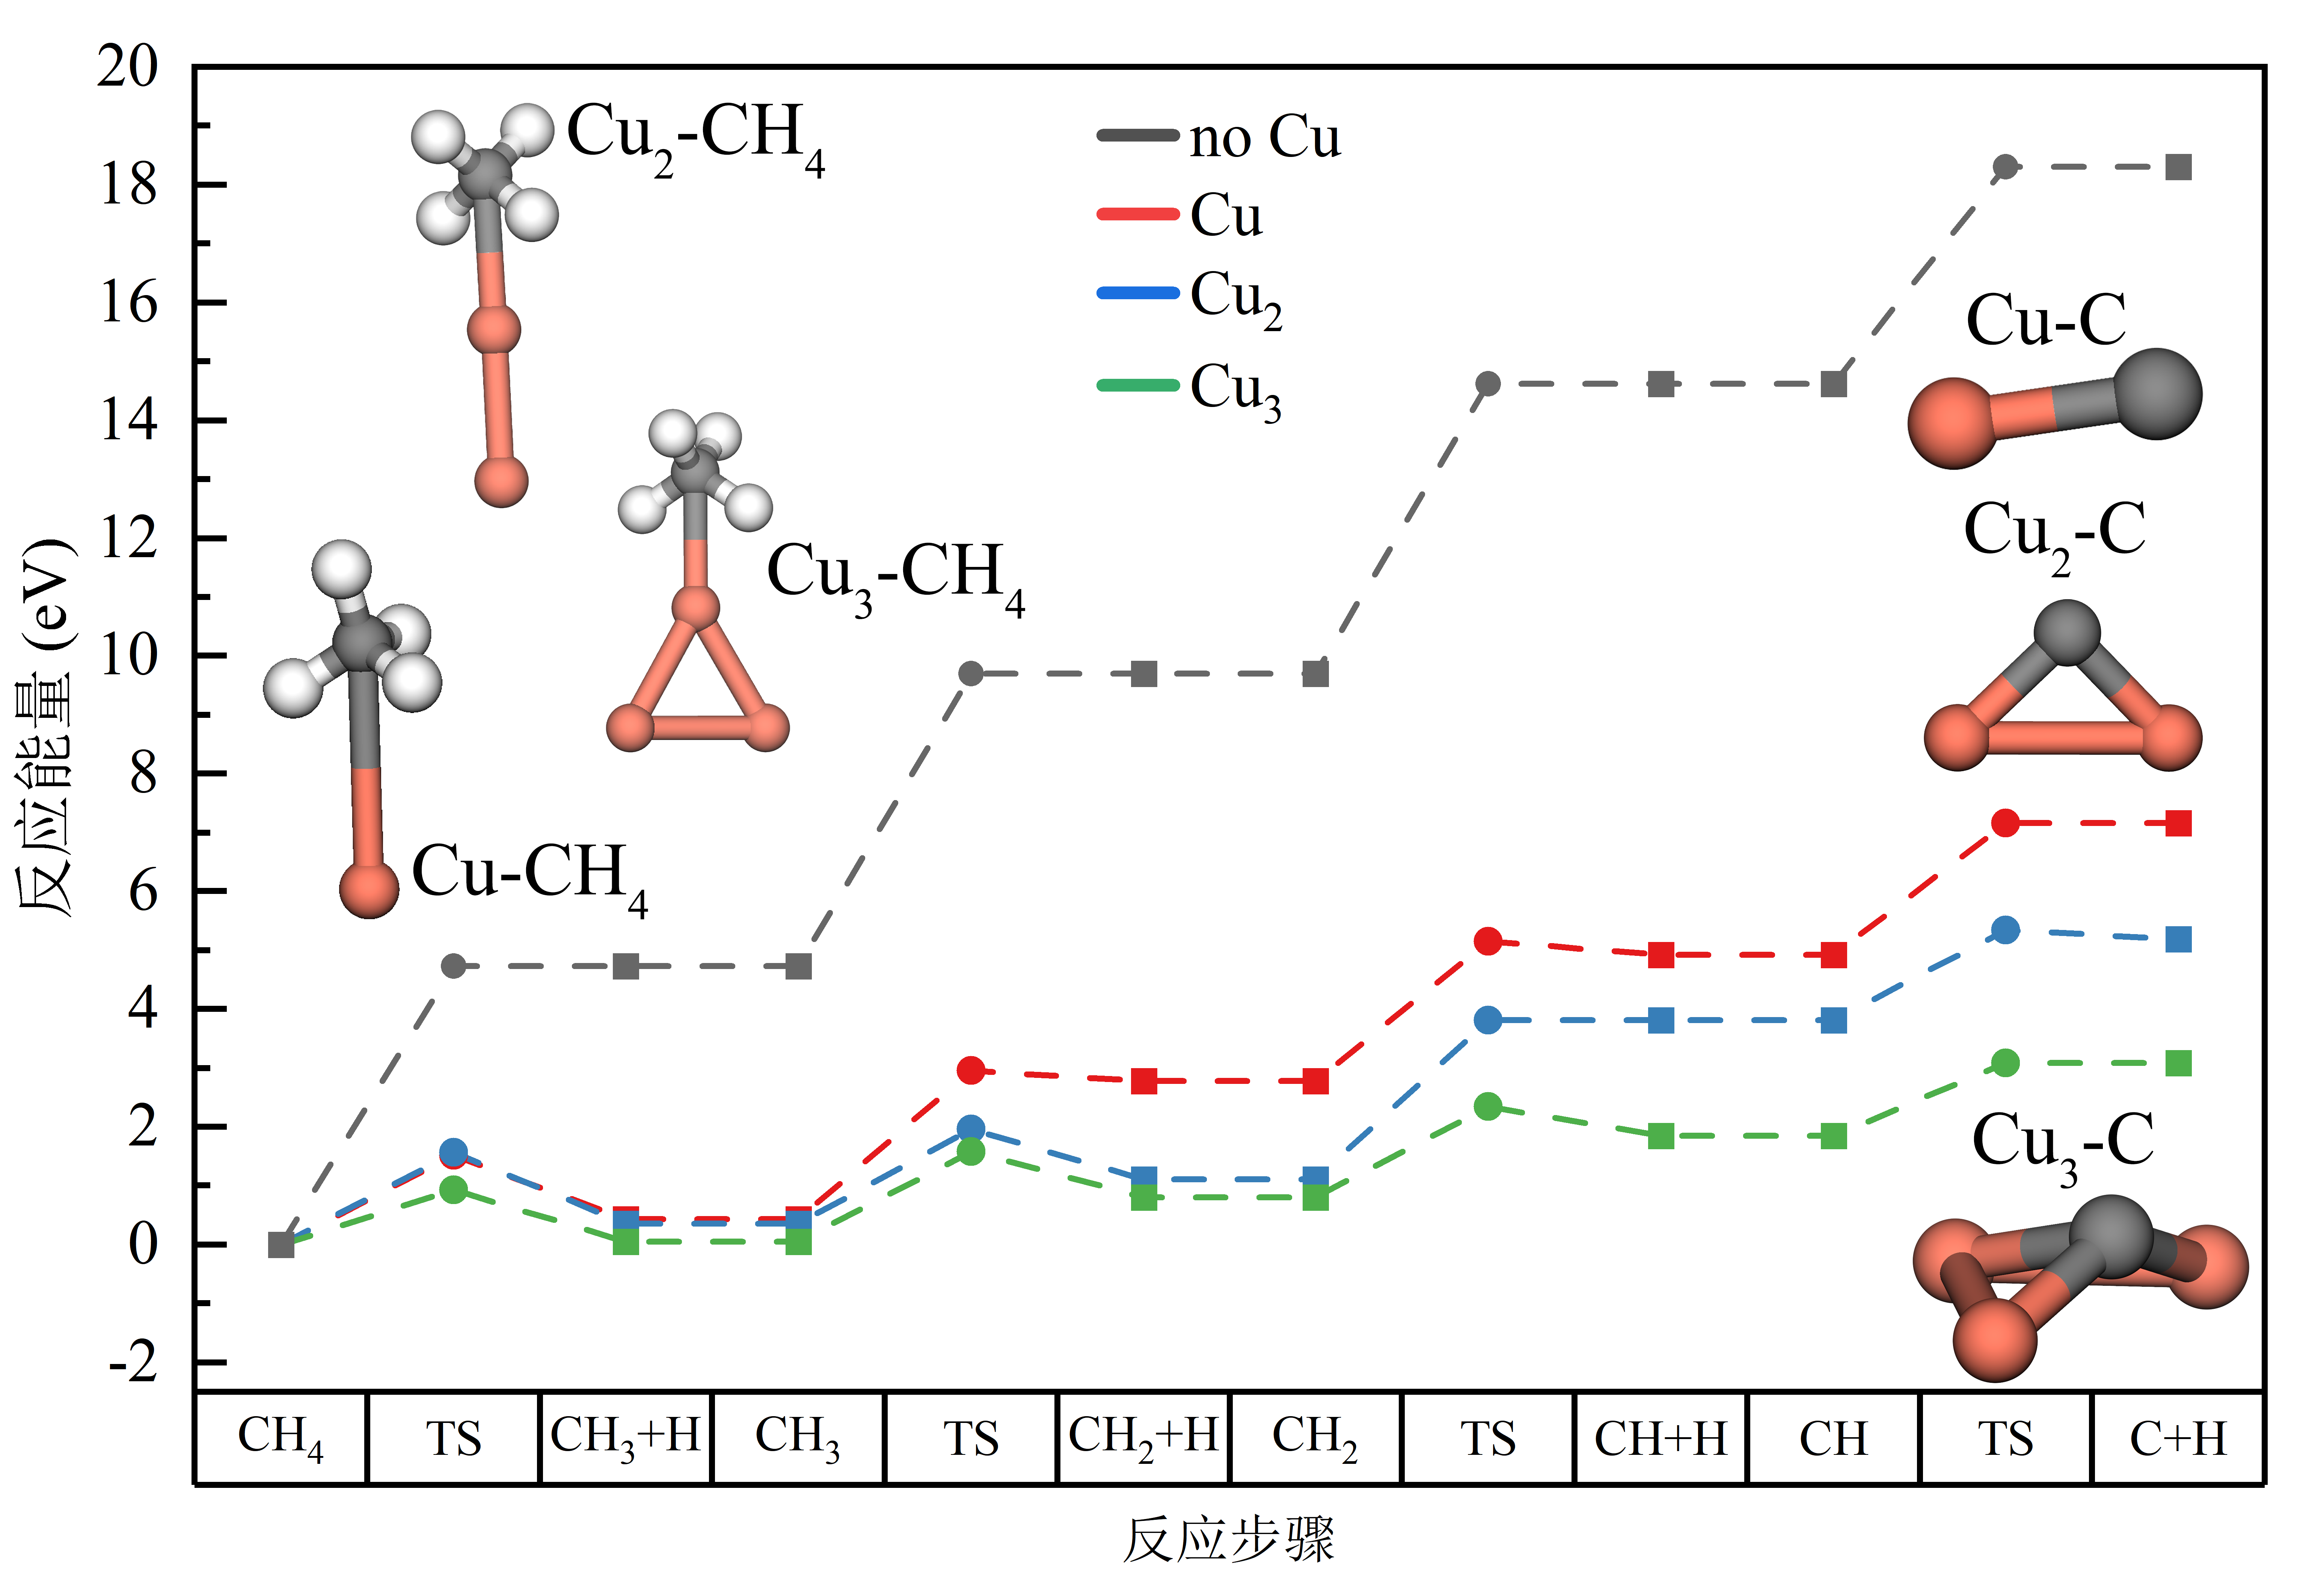
\includegraphics{pic/CG_DFT_CuCHx.png}
        \caption{\cemb{CH4}在\cemb{Cu}、\cemb{Cu2}、\cemb{Cu3}团簇以及无催化剂表面脱氢裂解的反应能和反应激活能变化情况。其中TS代表反应过渡态,其值为反应所需的激活能大小。在原子结构中,铜原子为橙色;碳原子为灰色;氢原子为白色。}
        \label{fig:CG_DFT_CuCHx}
    \end{figure}

    经过四步脱氢反应后,生长气氛中的\cemb{CH4}分子转变为活性的\cemb{C}原子,\cemb{C}原子在\cemb{Cu/h-BN}的表面作为碳源直接参与石墨烯的堆叠生长。如图\ref{fig:CG_DFT_CuCHx}所示,利用密度泛函理论方法,我们计算了在不同\cemb{Cu}团簇的表面,\cemb{CH4}四步脱氢裂解反应的反应激活能和反应能的变化情况。在图\ref{fig:CG_DFT_CuCHx}中,我们额外给出了无催化剂的参与下\cemb{CH4}脱氢裂解反应的能量变化曲线作为参考。

    可以看到,在没有\cemb{Cu}等催化剂的介入下\cemb{CH4}脱氢每步大约需要$\SI{3.69}{\electronvolt}\sim  \SI{4.9}{\electronvolt}$的激活能。如此高的反应激活需求使得反应气氛中的\cemb{CH4}难以直接裂解为\cemb{C}、\cemb{CH}等活性基团以供石墨烯的生长。当\cemb{Cu}团簇被引入作为催化剂后,密度泛函理论计算得到的\cemb{CH4}脱氢反应的激活能相比于无催化剂的情况产生了大幅度的下降。四步脱氢反应的激活能由无催化剂的最高约\SI{4.9}{\electronvolt}下降至\cemb{Cu}团簇作为催化剂的最高约\SI{2.7}{\electronvolt}。同时我们还可以发现,随着\cemb{Cu}团簇内包含的\cemb{Cu}原子的数目上升,\cemb{CH4}脱氢裂解反应的激活能和反应能由逐渐下降的趋势。

    通过和无催化剂辅助情况下\cemb{CH4}脱氢裂解的激活能和反应能进行比较,我们可以认为\cemb{Cu}团簇能够使\cemb{CH4}的脱氢裂解反应能量需求大幅下降。在表\ref{tab:CH4_cata}中,我们将\cemb{CH4}在\cemb{Cu}团簇表面和在平坦的\cemb{Cu(111)}衬底表面催化裂解过程的反应激活能($\energyVar{a}{}$)和反应能$\rm{\Delta} \it \energyVar{}{}$进行对比,探究\cemb{Cu}团簇的催化能力是否能够支撑石墨烯的生长。

    \begin{table}[htb]
    \def\aColWidth{0.20\textwidth}
    \def\bColWidth{0.10\textwidth}
    \def\cColWidth{0.12\textwidth}
    \def\dColWidth{0.12\textwidth}
    \def\eColWidth{0.12\textwidth}
    \def\fColWidth{0.12\textwidth}
    \def\abColwidth{0.3\textwidth}
    \caption{\mbox{\cemb{Cu}团簇和\cemb{Cu(111)}衬底表面\cemb{CH4}脱氢裂解反应的激活能$\energyVar{a}{}$和反应能$\Delta\energyVar{}{}$}}
    \label{tab:CH4_cata}
    \begin{tabular}{
        m{\aColWidth}
        >{\centering}m{\bColWidth}
        >{\centering}m{\cColWidth}
        >{\centering}m{\dColWidth}
        >{\centering}m{\eColWidth}
        >{\centering\arraybackslash}m{\fColWidth}
    }
    \toprule
    \multicolumn{2}{c}{\multirow{3.5}{*}{反应步骤}}&\multicolumn{3}{c}{\cemb{Cu}团簇构型}&\shortstack[c]{\cemb{Cu}衬底\\表面}\\
    \cmidrule{3-6}
    &&\cemb{Cu}团簇&\cemb{Cu2}团簇&\cemb{Cu3}团簇&\shortstack[c]{\cemb{Cu(111)}\\表面\citing{RN789-2013}}\\
    \midrule
    \multirow{2}{\abColwidth}{\cemb{CH4 -> CH3 + H}} & $\energyVar{a}{}\ \ (\si{\electronvolt})$&1.51&1.57&0.92&1.88\\
    &$\Delta \energyVar{}{}\;(\si{\electronvolt})$&0.43&0.35&0.05&0.86\\
    \multirow{2}{\abColwidth}{\cemb{CH3 -> CH2 + H}} &$\energyVar{a}{}\ \ (\si{\electronvolt})$&2.52&1.61&1.54&1.47\\
    &$\Delta \energyVar{}{}\;(\si{\electronvolt})$&2.34&0.76&1.53&1.05\\
    \multirow{2}{\abColwidth}{\cemb{CH2 -> CH + H}} &$\energyVar{a}{}\ \ (\si{\electronvolt})$&2.37&2.70&1.53&1.05\\
    &$\Delta \energyVar{}{}\;(\si{\electronvolt})$&2.15&2.70&1.05&0.32\\
    \multirow{2}{\abColwidth}{\cemb{CH\hphantom{$_{2}$} -> C + H}} &$\energyVar{a}{}\ \ (\si{\electronvolt})$&2.25&1.53&1.23&2.21\\
    &$\Delta \energyVar{}{}\;(\si{\electronvolt})$&2.25&1.38&1.23&1.20\\
    \midrule
    \multirow{2}{\abColwidth}{\shortstack{总反应\\\cemb{CH4 -> C + 4H}}}&$\energyVar{a}{}\ \ (\si{\electronvolt})$&2.52&2.70&1.54&2.21\\
    &$\Delta \energyVar{}{}\;(\si{\electronvolt})$&7.17&5.19&3.09&3.08\\
    \bottomrule
    \end{tabular}
\end{table}

    从激活能$\energyVar{a}{}$的计算分布来看\cemb{CH3 -> CH2 + H}为\cemb{CH4}的脱氢裂解反应在\cemb{Cu}团簇和\cemb{Cu3}团簇表面的决速步,需要分别翻越\SI{2.52}{\electronvolt}和\SI{1.53}{\electronvolt}的能量。对于\cemb{CH4}在\cemb{Cu2}表面的脱氢催化反应,激活能最大的脱氢步骤为\cemb{CH2 -> CH + H},此步的激活能为\SI{2.70}{\electronvolt}。在我们所计算的代表\cemb{Cu}蒸气的三种\cemb{Cu}团簇中,\cemb{Cu3}团簇的激活能低于\cemb{CH4}在\cemb{Cu}衬底表面脱氢裂解的激活能\SI{2.21}{\electronvolt}。在\cemb{Cu(001)}衬底的表面\cemb{CH4}裂解的决速步为最后一步\cemb{CH -> C + H}。因此相比于直接提供\cemb{C}原子,在\cemb{Cu(111)}衬底的表面\cemb{CH4}的脱氢裂解还能提供大量的\cemb{CH}基团进行石墨烯的成核生长。而在\cemb{Cu3}团簇的表面,由\cemb{CH4 -> CH + 3H}生成\cemb{CH}集团的反应过程的所需的最高激活能$\energyVar{a}{}=\SI{1.54}{\electronvolt}$,仅仅比\cemb{Cu(111)}表面同样生成\cemb{CH}的反应激活能(\SI{1.47}{\electronvolt})高\SI{0.07}{\electronvolt}。因此我们可以认为在\cemb{Cu3}团簇的表面,\cemb{CH4}裂解生成\cemb{CH}的的能力仅稍逊与\cemb{Cu(111)}的表面,同样能够提供大量的\cemb{CH}用于石墨烯在\cemb{Cu/h-BN}表面的直接成核生长。 

    进一步考虑\cemb{CH4}脱氢裂解的反应能情况。在\cemb{Cu}团簇的表面,\cemb{CH4}裂解的总应能随着团簇内包含\cemb{Cu}数量的上升由在\cemb{Cu}表面的\SI{7.17}{\electronvolt}下降至在\cemb{Cu3}表面的\SI{3.09}{\electronvolt},接近于在\cemb{Cu(111)}表面的\SI{3.08}{\electronvolt}的反应吸热。更低的反应能意味着有更多的\cemb{CH4}在热动能的推动下转化为\cemb{C},为\cemb{Cu/h-BN}表面生长的石墨烯提供更为充足的碳源。
    
    \begin{figure}[htb]
        \subfloat[]{
            \includegraphics[width=0.45\textwidth]{pic/CG_DFT_Cu3-CH4-CH3.png}
        }
        \subfloat[]{
            \includegraphics[width=0.45\textwidth]{pic/CG_DFT_Cu3-CH3-CH2.png}
        }\\[-0.5ex]
        \subfloat[]{
            \includegraphics[width=0.45\textwidth]{pic/CG_DFT_Cu3-CH2-CH.png}
        }
        \subfloat[]{
            \includegraphics[width=0.45\textwidth]{pic/CG_DFT_Cu3-CH-C.png}
        }
        \caption{\cemb{Cu3}团簇表面\cemb{CH4}脱氢解离的四个反应步骤的反应过程以及能量变化。(a)\cemb{CH4 -> CH3 + H}反应;(b)\cemb{CH3 -> CH2 + H}反应;(c)\cemb{CH2 -> CH + H}反应;(d)\cemb{CH -> C + H}反应。在原子结构中,铜原子为橙色;碳原子为灰色;氢原子为白色。}
        \label{fig:CG_DFT_Cu3-CH4-C}
    \end{figure}

    在图\ref{fig:CG_DFT_Cu3-CH4-C}中,我们绘制了在\cemb{Cu3}团簇表面\cemb{CH4}脱氢解离的四个反应步骤的反应过程以及能量变化图。可以看到,在\cemb{Cu3}团簇的表面,\cemb{CH4}吸附在\cemb{Cu}三角形的顶点处,\cemb{CH4}脱氢的过程也在这个顶点\cemb{Cu}原子上发生。在\cemb{CH4}脱氢为\cemb{CH3}的过程中,\cemb{CH4}中的一个\cemb{H}原子朝\cemb{Cu}三角形的一个棱边运动,剩下的\cemb{CH3}部分也在\cemb{Cu}顶点原子的作用下朝三角形的另一个边运动。这个过程需要吸收\SI{0.92}{\electronvolt}的能量跨越势垒。当脱氢的过程完成后,\cemb{CH3}和脱离的\cemb{H}原子分别立于\cemb{Cu3}团簇三角形的两边。\cemb{C}和脱离的\cemb{H}原子分别和两个\cemb{Cu}原子成键,这步反应需要吸收\SI{0.05}{\electronvolt}的能量。对于\cemb{CH4}在\cemb{Cu3}团簇上脱氢裂解的决速步,\cemb{CH3 -> CH2 + H}反应,在初始状态下\cemb{CH3}在\cemb{Cu3}的\cemb{Cu}三角形顶角吸附。在脱氢的过程中,\cemb{CH2}原子团首先移动到\cemb{Cu3}三角形的棱边处和两个顶角的\cemb{Cu}原子成键,此时脱离的\cemb{H}原子在原顶角的位置与\cemb{Cu}相连。移动到这个过渡态至少需要吸收\SI{1.54}{\electronvolt}的能量。随后分离的\cemb{H}原子继续向\cemb{Cu3}三角形的棱边移动,释放出部分吸收的热量,最终在另一个棱边处完成此步脱氢反应,最终消耗\SI{0.76}{\electronvolt}的能量。
    
    在\cemb{CH2}的脱氢反应中,\cemb{CH2}原子团稳定在\cemb{Cu3}三角形的棱边处。反应开始后,\cemb{CH}原子团和分离的\cemb{H}原子分别从\cemb{Cu3}三角形面外绕行的方式进行运动。在攀上了势垒为\SI{1.53}{\electronvolt}的过渡态后,\cemb{CH}原子团位于\cemb{Cu3}三角形表面的中心位置,\cemb{C}原子同时与三个\cemb{Cu}原子具有相互作用,而\cemb{H}原子保持在与一个顶角\cemb{Cu}相连的位置,但也朝向\cemb{Cu3}三角形面的法线方向。随后,\cemb{H}原子继续向\cemb{Cu3}三角形的棱边运动,最终在棱边处于两个顶角的\cemb{Cu}原子成键。此步反应的反应吸热为\SI{1.05}{\electronvolt}。在最终的脱氢步中,过渡态和反应终态极为接近,\cemb{CH}原子团吸收了\SI{1.23}{\electronvolt}的能量后与最后一个\cemb{H}原子分离,形成具有高活性的\cemb{C}吸附原子。
    
    \subsection{\cemb{h-BN}表面石墨烯的生长演化机理}
    
    当前驱体\cemb{CH4}在\cemb{Cu}蒸气的作用下在\cemb{Cu/h-BN}的表面脱氢、裂解成活性\cemb{C}、\cemb{CH}等物质。这些具有活性的含碳化合物在\cemb{Cu/h-BN}的表面进一步沉积、成核、生长成为石墨烯。为了进一步探究在\cemb{Cu/h-BN}表面的生长机理,我们使用第一性原理的方法计算了\cemb{C}团簇在\cemb{Cu/h-BN}表面的成核生长过程。
    
    在计算过程中,我们使用石墨烯的平均\cemb{C}原子形成能
    $$\energyVar{f}{}=\left(\energyVar{total}{}-\energyVar{Cu/h-BN}{}-N\times \energyVar{C}{}\right)\slash N$$
    来表征不同\cemb{C}团簇的能级水平。其中,$\energyVar{total}{}$为在\cemb{Cu/h-BN}表面生长\cemb{C}团簇后整个体系的总能量;$\energyVar{Cu/h-BN}{}$为单独\cemb{Cu/h-BN}衬底的能量;$N$为形成\cemb{C}团簇的\cemb{C}原子的个数;$\energyVar{C}{}$为\cemb{C}原子的能量。

    同时,先前的研究表明,石墨烯在\cemb{Cu}衬底表面生长的早期阶段中\cemb{C}团簇中的\cemb{C}原子更容易形成sp的杂化形式,而不是形成在石墨烯中常见的$\rm sp^2$杂化\citing{RN822-2011}。因此,除了石墨烯的六边形团簇外、我们在石墨烯生长阶段的早期还同时考虑了由sp杂化\cemb{C}原子组成的线形和环形\cemb{C}团簇。


    \begin{figure}[htb]
        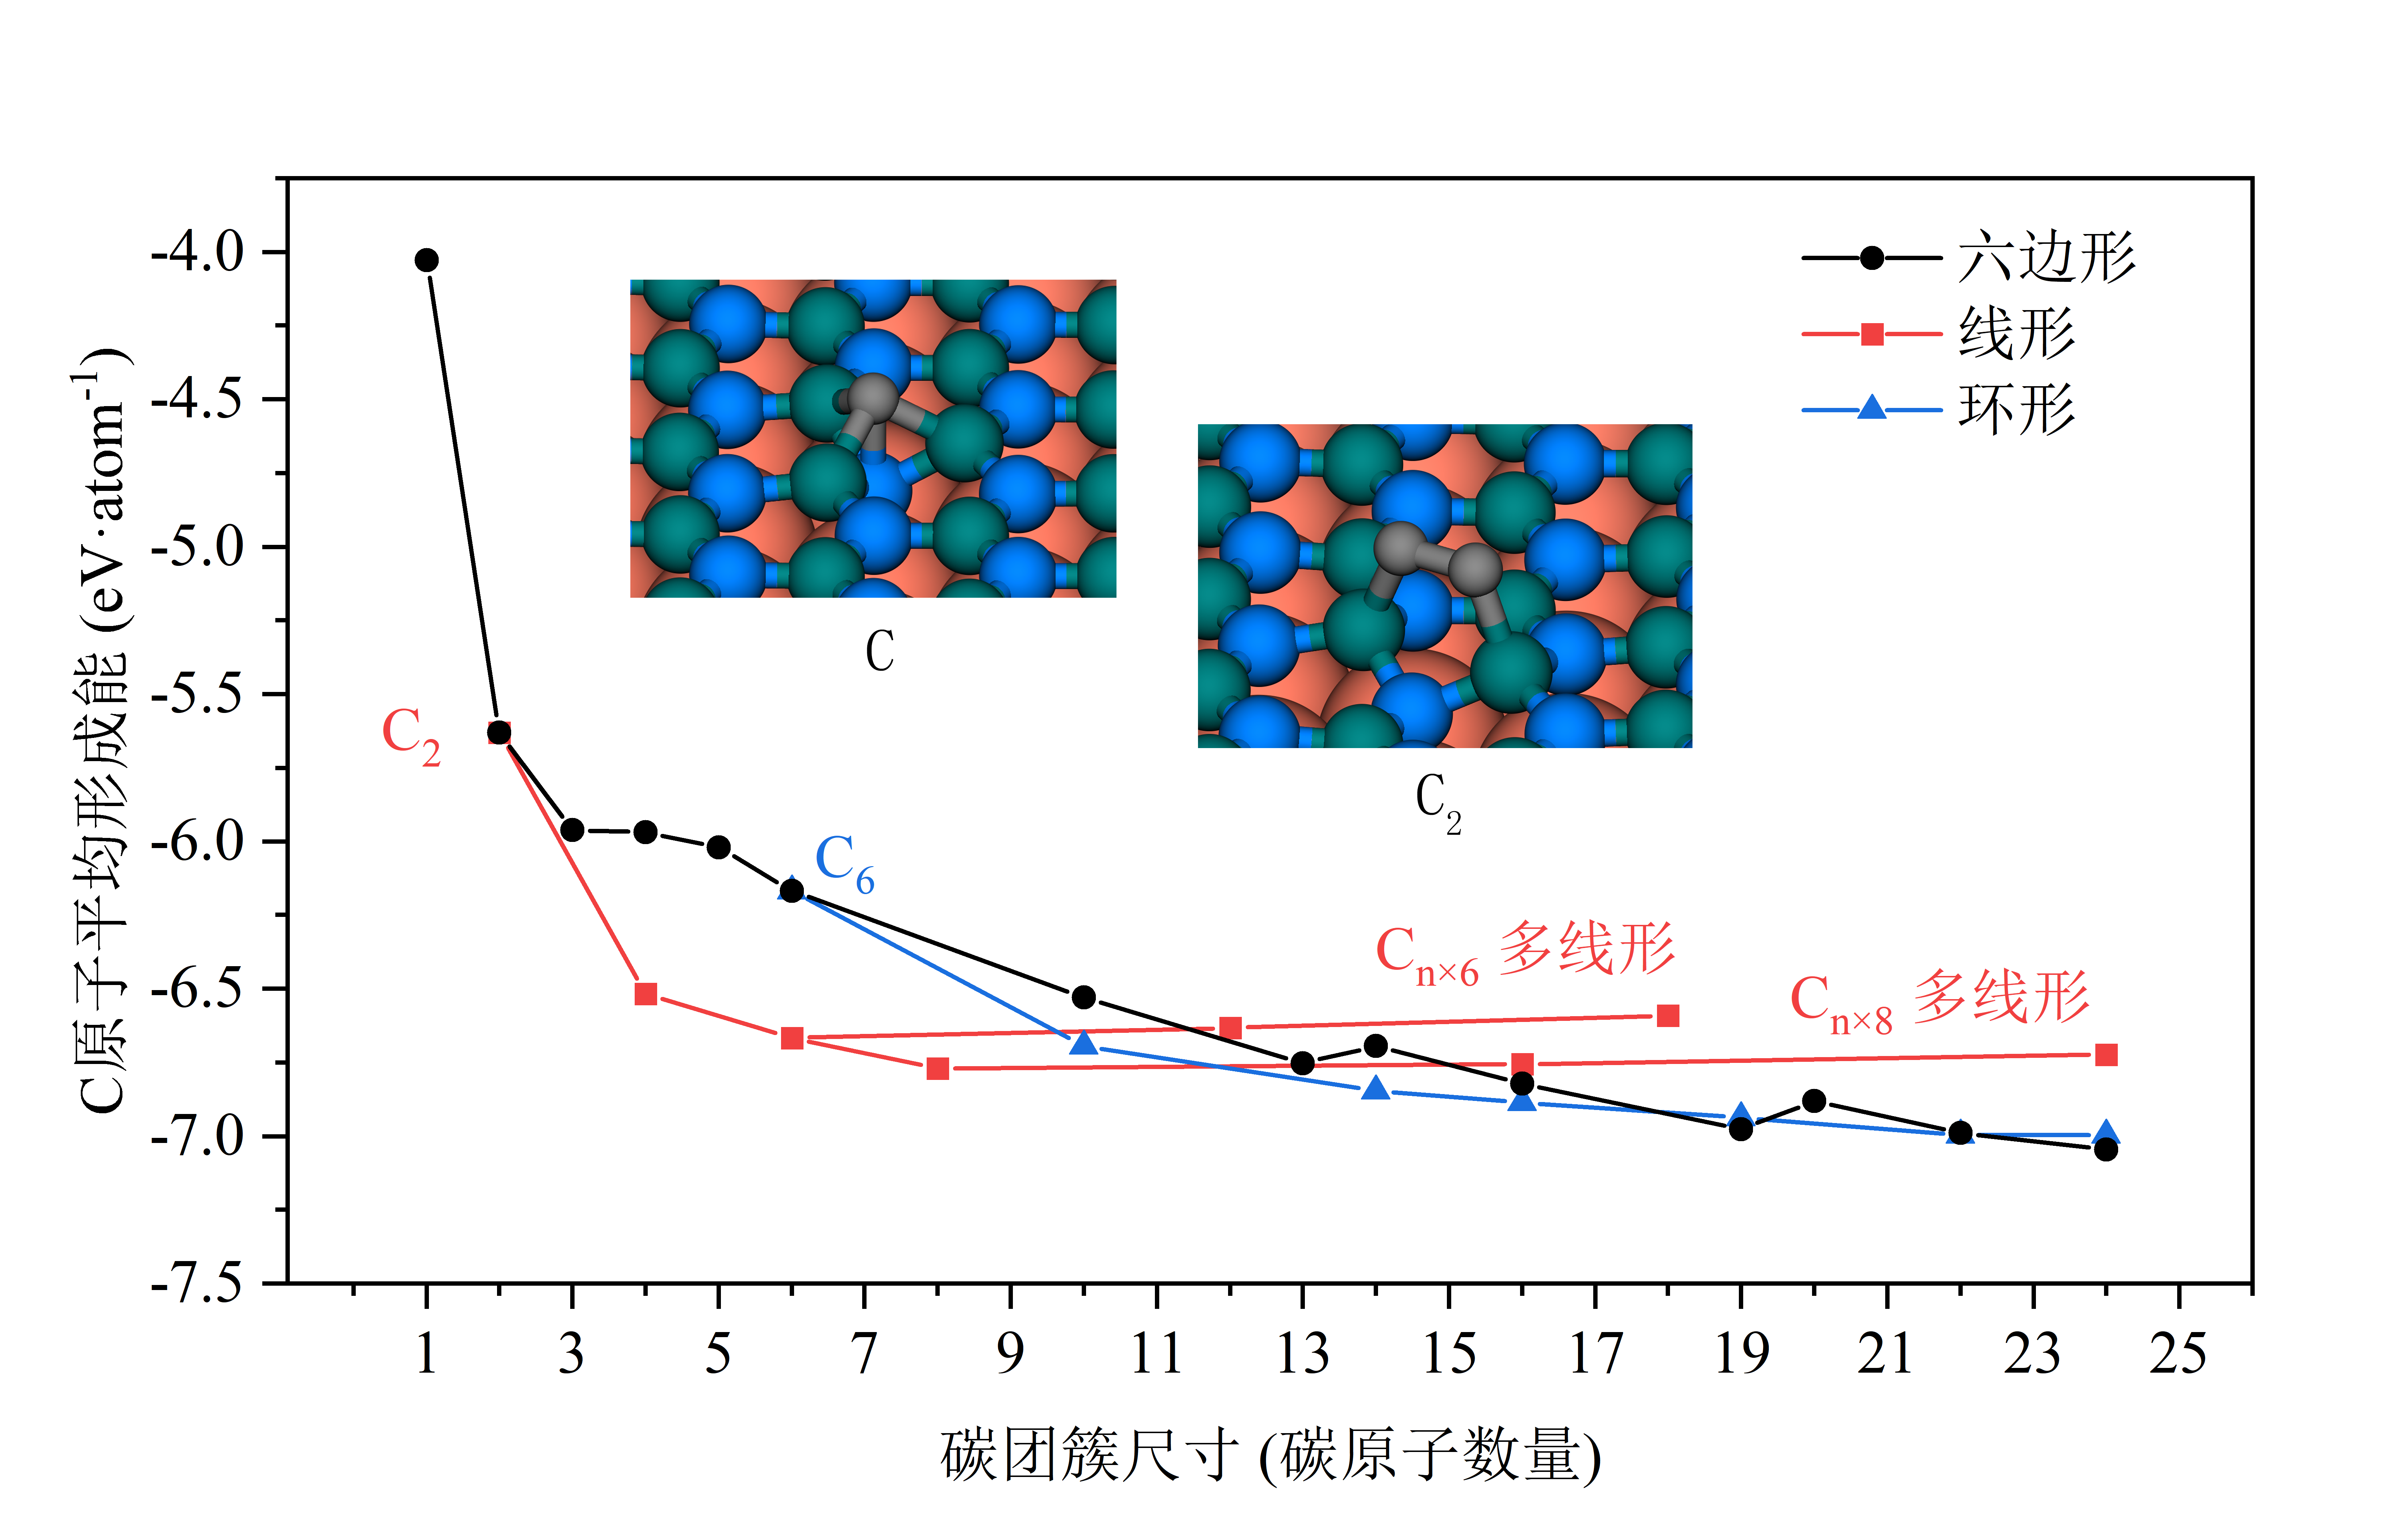
\includegraphics{pic/CG_DFT_C_cluster_onBN.png}
        \caption{$1 \sim 24$个\cemb{C}原子的六边形、线形、环形的\cemb{C}团簇在\cemb{Cu/h-BN}表面生长的形成能以及\cemb{C}单原子、\cemb{C2}团簇在\cemb{Cu/h-BN}表面生长的原子结构。原子结构图中,铜原子为橙色;氮原子为蓝色;硼原子为绿色;碳原子为灰色。}
        \label{fig:CG_DFT_C_cluster_onBN}
    \end{figure}

    在图\ref{fig:CG_DFT_C_cluster_onBN}中,我们给出了包含$1 \sim 24$个\cemb{C}原子的六边形、线形、环形的\cemb{C}团簇在\cemb{Cu/h-BN}表面生长的形成能。我们可以看到,对于单个\cemb{C}原子在\cemb{Cu/h-BN}表面吸附,形成能为\SI{-4.02}{\electronvolt\per\atom}。单个的\cemb{C}原子吸附在\cemb{h-BN}表面的\cemb{N}原子上方,并且与下方的\cemb{N}原子以及斜侧方的三个\cemb{B}原子均有成键。\cemb{C}原子在\cemb{Cu/h-BN}表面的吸附破坏了\cemb{h-BN}单层的平面结构,使得吸附位点的\cemb{N}原子向\cemb{Cu}衬底沉降,与表面的\cemb{Cu}原子产生键合。

    在\cemb{Cu/h-BN}表面吸附的单个\cemb{C}原子在与生长环境或者\cemb{Cu/h-BN}表面的另一个\cemb{C}原子结合后,可以形成\cemb{C2}团簇,形成能下降至\SI{-5.63}{\electronvolt\per\atom}。双原子的\cemb{C2}团簇之间较强的\cemb{C-C}键使得原本吸附在\cemb{N}原子上方的\cemb{C}吸附原子移动到\cemb{B}原子的上方,在\cemb{h-BN}表面锯齿晶向(zigzag)相邻的两个\cemb{B}原子上方形成\cemb{C2}团簇。\cemb{C2}团簇的形成将下方的\cemb{B}原子略微拉扯出\cemb{h-BN}平面。


    \begin{figure}[htb]
        \subfloat[]{
            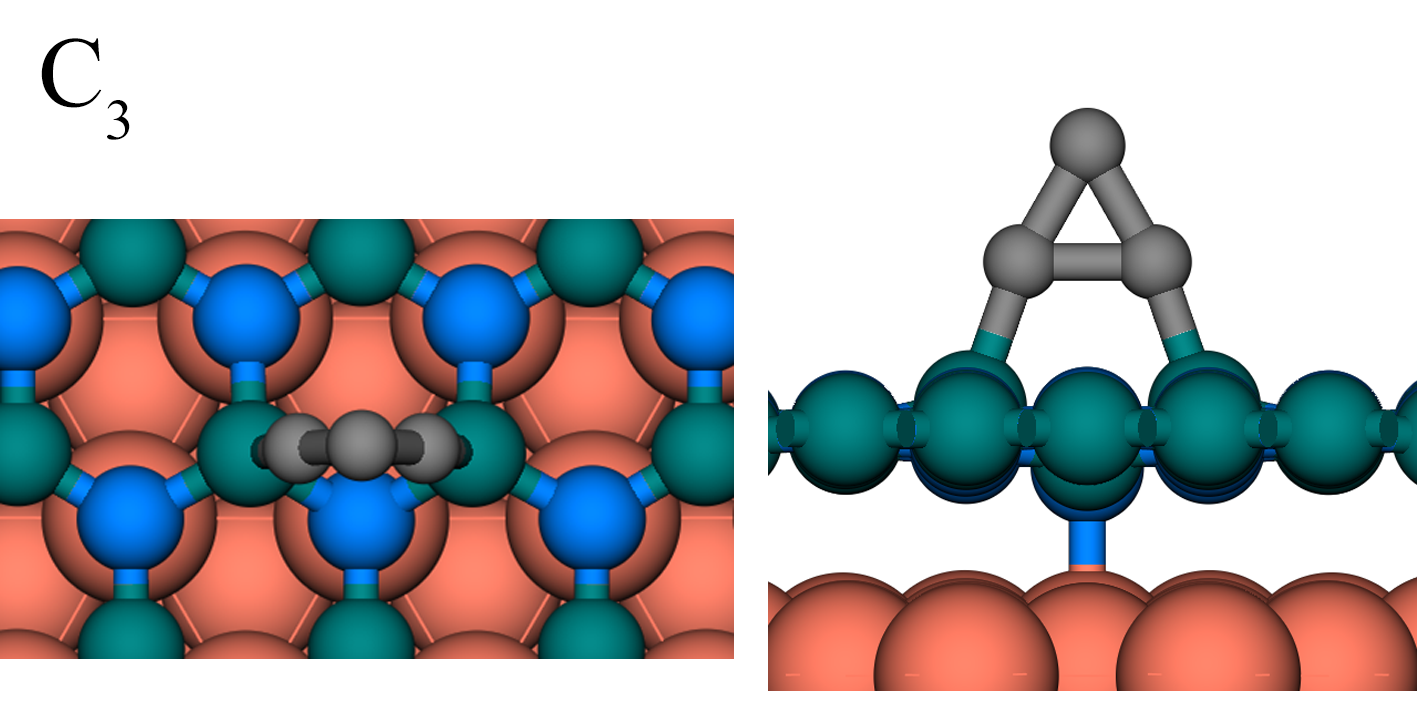
\includegraphics{pic/CG_structure_3C.png}
            \label{fig:CG_structure_3C}
        }
        \subfloat[]{
            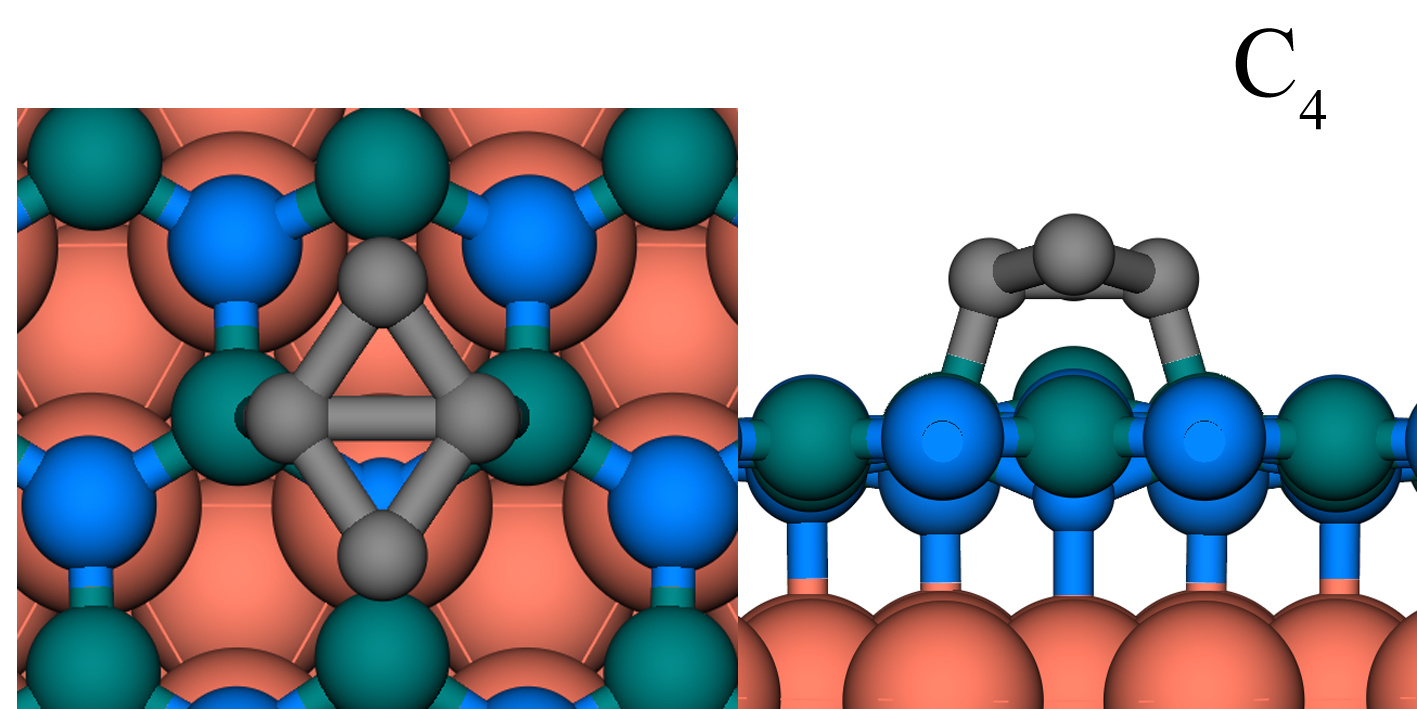
\includegraphics{pic/CG_structure_4C.png}
            \label{fig:CG_structure_4C}
        }\\[-0.5ex]
        \subfloat[]{
            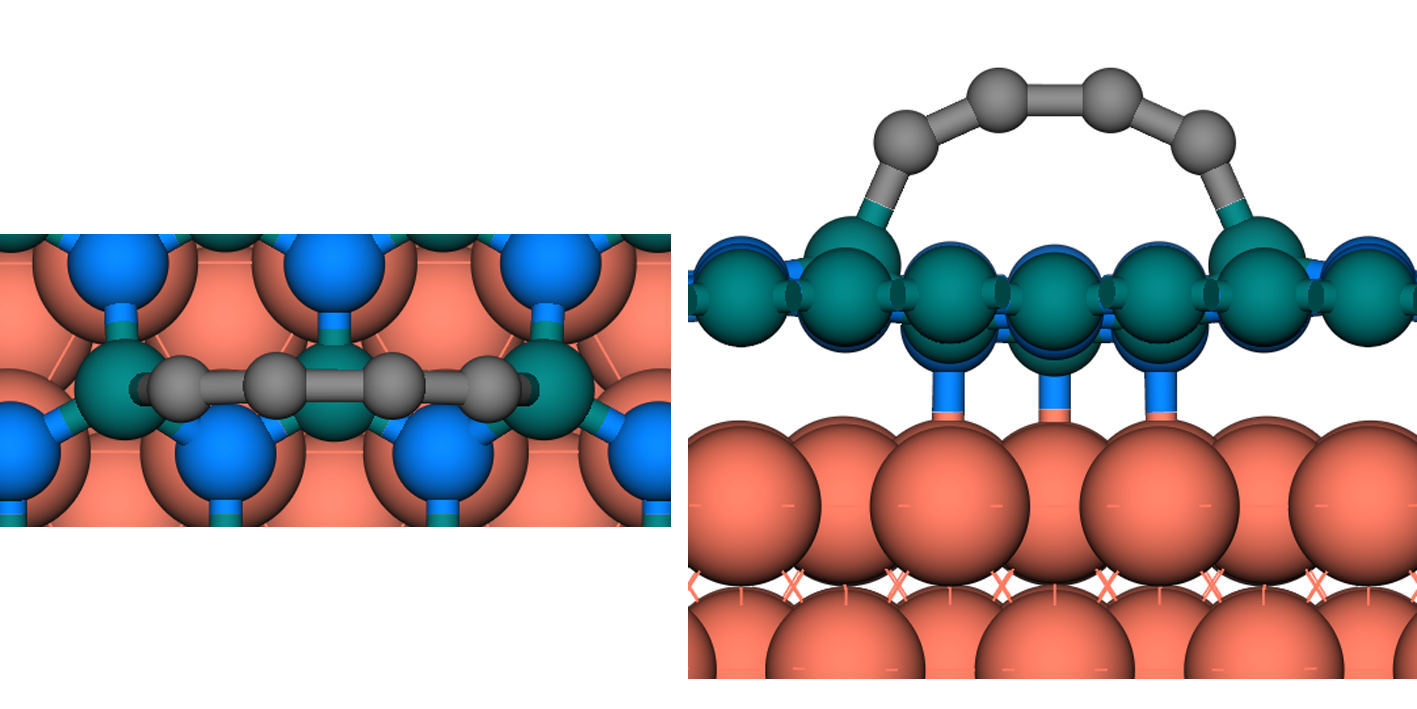
\includegraphics{pic/CG_structure_4CL.png}
            \label{fig:CG_structure_4CL}
        }
        \subfloat[]{
            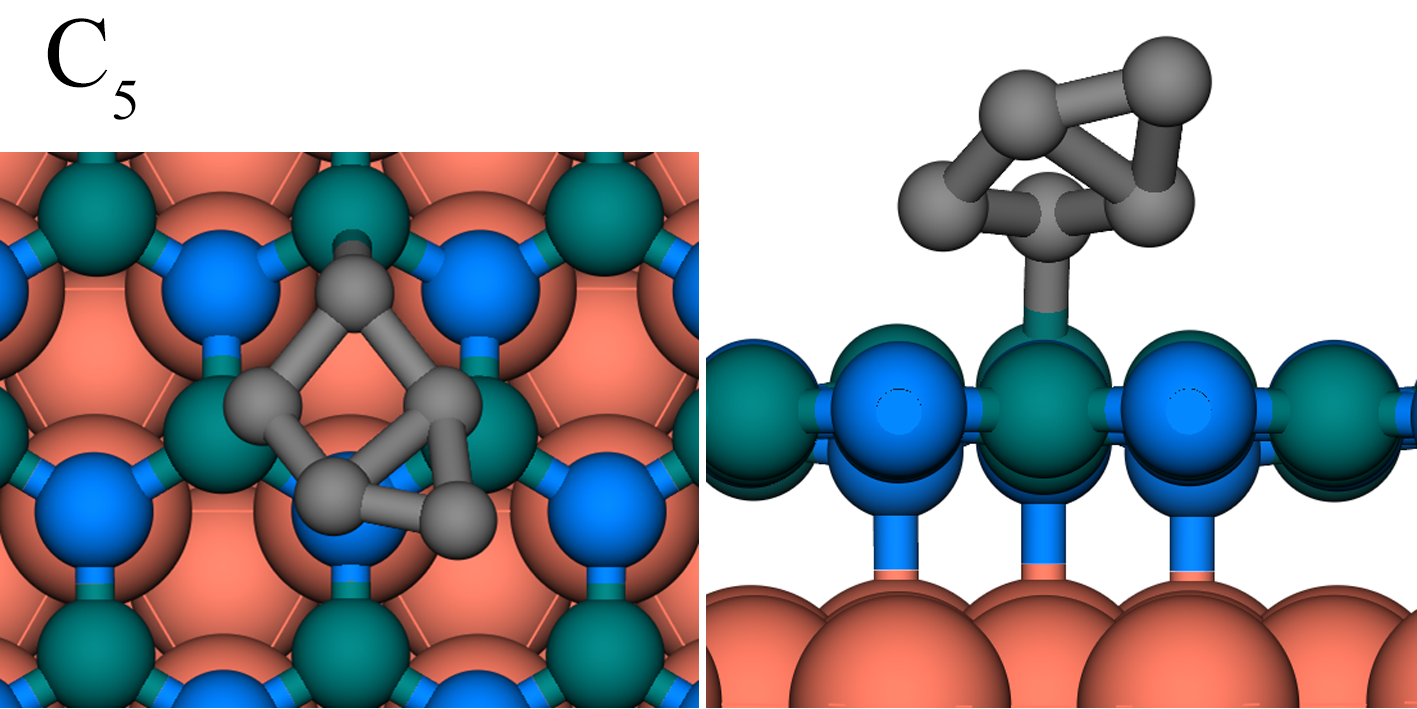
\includegraphics{pic/CG_structure_5C.png}
            \label{fig:CG_structure_5C}
        }
        \caption{\cemb{Cu/h-BN}表面\cemb{C}团簇的原子结构图。(a)\cemb{C3}团簇;(b)\cemb{C4}团簇;(c)\cemb{C4}线形团簇;(d)\cemb{C5}团簇。原子结构图中,铜原子为橙色;氮原子为蓝色;硼原子为绿色;碳原子为灰色。}
        \label{fig:CG_structure_3-5C}
    \end{figure}

    第三个\cemb{C}原子加入\cemb{C}团簇后,\cemb{C3}团簇在\cemb{h-BN}表面呈现出直立的三角形形貌(\ref{fig:CG_structure_3C})。在直立的三角形结构下,\cemb{C3}团簇的\cemb{C}原子平均形成能下降至\SI{-5.96}{\electronvolt\per\atom}。此时,\cemb{C3}三角形团簇的下方两个顶点\cemb{C}原子与\cemb{h-BN}表面的相邻的两个\cemb{B}原子成键。三角形的边长略小于相邻两个\cemb{B}原子之间的距离。包含四个\cemb{C}原子的\cemb{C4}团簇恢复了平面的结构(\ref{fig:CG_structure_4C}),在\cemb{h-BN}表面形成菱形的形貌。这种菱形结构的\cemb{C4}团簇的平均\cemb{C}原子结合能为\SI{-5.97}{\electronvolt\per\atom},仅比\cemb{C3}三角形团簇下降了\SI{0.01}{\electronvolt\per\atom}。相比之下,由四个\cemb{C}原子组成的\cemb{C4}线形团簇具有非常大的形成能下降(\ref{fig:CG_structure_4CL})。\cemb{C4}线形团簇类似于\cemb{2}团簇,线形的两端与\cemb{h-BN}表面的\cemb{B}原子成键,中央的\cemb{C}原子上翘,形成类似于弓形的结构。在我们的形成能计算中,\cemb{C4}线形团簇在\cemb{h-BN}的表面以与锯齿边的平行的方向形成,平均\cemb{C}原子形成能为\SI{-6.52}{\electronvolt\per\atom},远低于形成平面菱形结构的\cemb{C4}团簇。从\cemb{C4}团簇开始,线形的\cemb{C}团簇在\cemb{h-BN}的表面相比于六边形、环形等二维结构的\cemb{C}团簇具有相当的形成能优势。在平面菱形的\cemb{C4}团簇上进一步添加一个\cemb{C}原子形成具有平面构型的\cemb{C5}团簇\ref{fig:CG_structure_5C},其平均\cemb{C}原子结合能仅下降至\SI{-6.02}{\electronvolt\per\atom}。此时的\cemb{C5}团簇的一个顶角从\cemb{h-BN}的表面脱离并向上翘起,以释放团簇内\cemb{C}原子之间的应力,维持sp2杂化的\cemb{C}原子之间的平面结构。

    当\cemb{C}团簇中的\cemb{C}原子数量上升到6个,即可形成具有类石墨烯结构的\cemb{C6}六边形团簇。在\cemb{Cu/h-BN}表面上,\cemb{C6}六边形团簇的两个相对的\cemb{C}原子与\cemb{h-BN}扶手椅边(armchair)方向的两个\cemb{B}原子成键,其余的四个\cemb{C}原子上翘。\cemb{C6}六边形团簇的六元环整体形成舟形的原子结构(图\ref{fig:CG_structure_6CH})。此时的\cemb{C}原子平均形成能为\SI{-6.17}{\electronvolt\per\atom},相比于平面形的\cemb{C4}、\cemb{C5}团簇有较大的形成能下降。但包含六个sp杂化\cemb{C}原子的\cemb{C6}线形团簇的平均形成能为\SI{-6.77}{\electronvolt\per\atom},相比于\cemb{C6}六边形团簇具有更好的能量优势。\cemb{C6}线形团簇同样处于\cemb{h-BN}锯齿边的\cemb{B}原子的上方,整个\cemb{C6}线形团簇在\cemb{h-BN}的表面横跨4个\cemb{B}原子,两端的\cemb{C}原子与\cemb{B}原子成键,整体呈现出弓形的原子结构(图\ref{fig:CG_structure_6CL})。

    \begin{figure}[htb]
        \subfloat[]{
            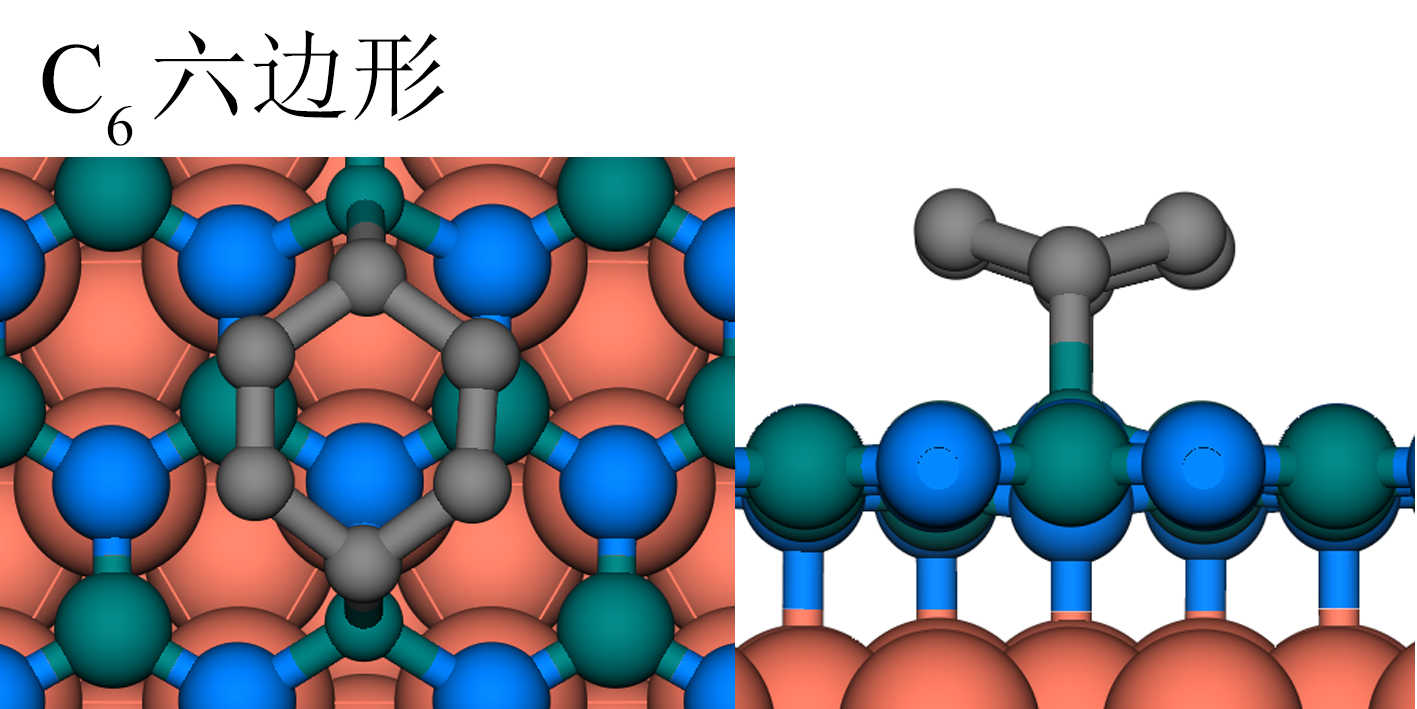
\includegraphics{pic/CG_structure_6CH.png}
            \label{fig:CG_structure_6CH}
        }
        \subfloat[]{
            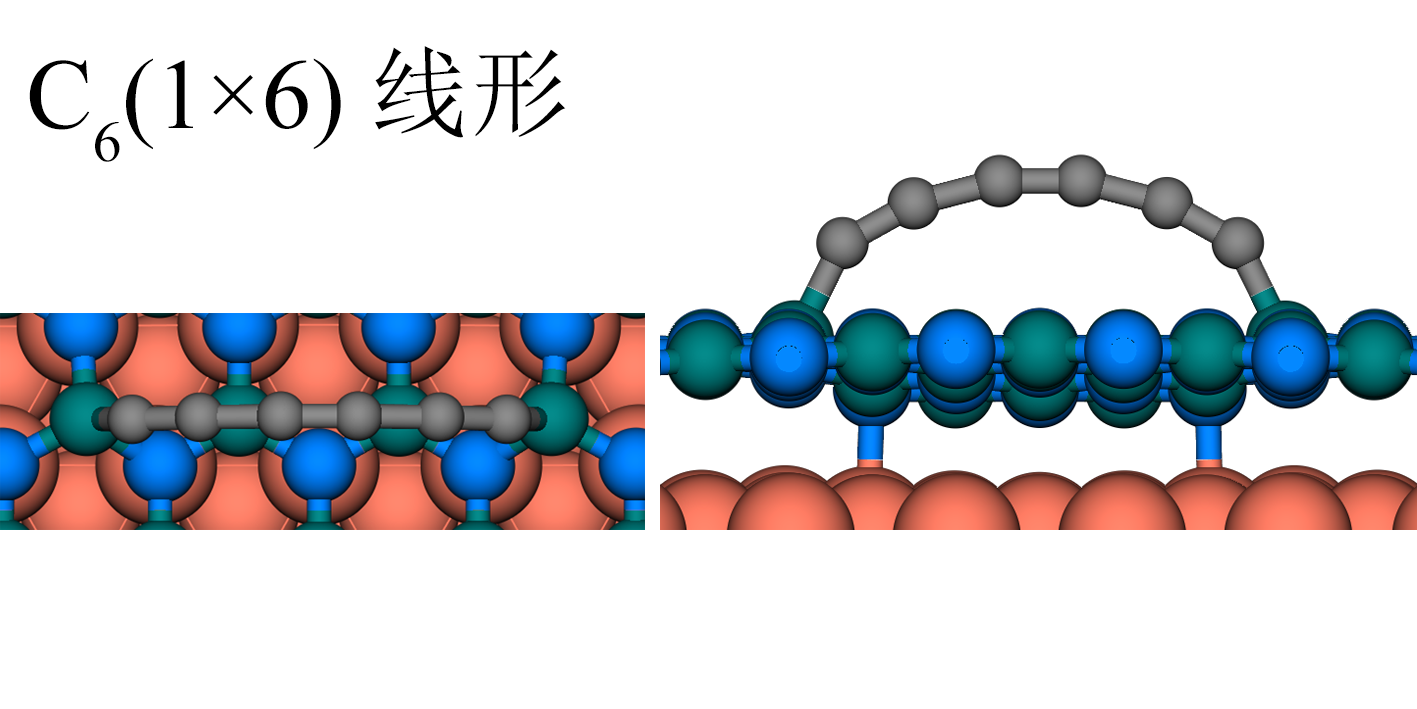
\includegraphics{pic/CG_structure_6CL.png}
            \label{fig:CG_structure_6CL}
        }\\[-0.5ex]
        \subfloat[]{
            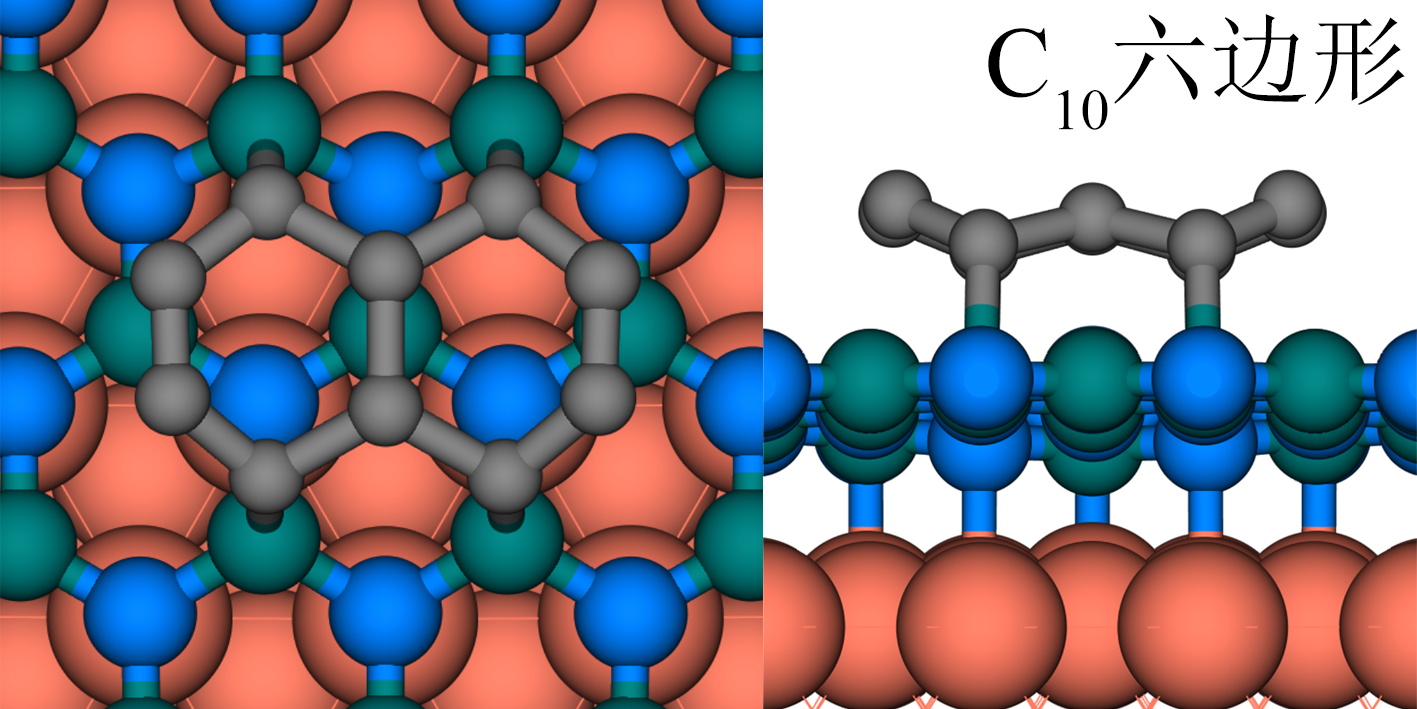
\includegraphics{pic/CG_structure_10CH.png}
            \label{fig:CG_structure_10CH}
        }
        \subfloat[]{
            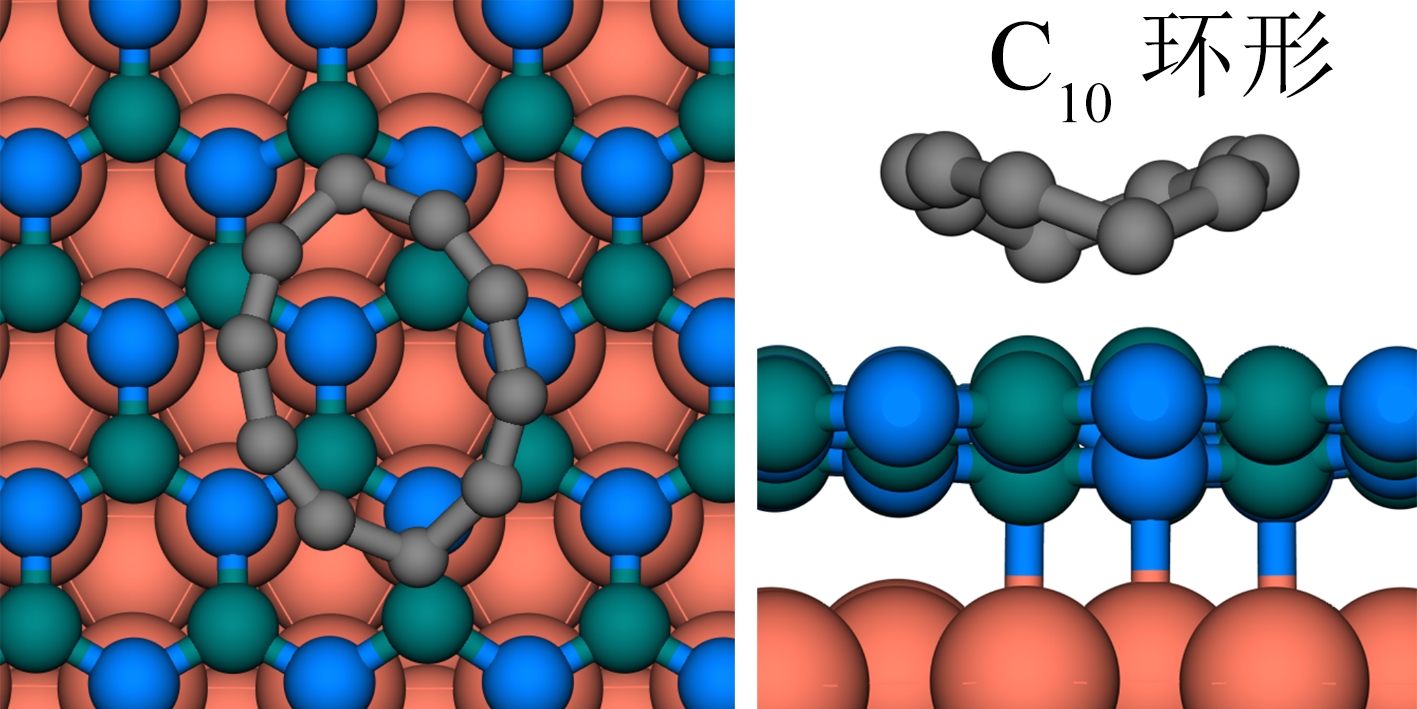
\includegraphics{pic/CG_structure_10CR.png}
            \label{fig:CG_structure_10CR}
        }
        \caption{\cemb{Cu/h-BN}表面\cemb{C}团簇的原子结构图。(a)\cemb{C6}六边形团簇;(b)\cemb{6}线形团簇;(c)\cemb{C10}六边形团簇;(d)\cemb{C10}环形团簇。原子结构图中,铜原子为橙色;氮原子为蓝色;硼原子为绿色;碳原子为灰色。}
        \label{fig:CG_CG_structure_6-10C}
    \end{figure}

    当\cemb{C}团簇中的\cemb{C}原子数量上升到10个,平面结构的\cemb{C}团簇从\cemb{C6}六边形团簇进一步分裂出环形的原子构型。\cemb{C10}环形团簇的\cemb{C}原子平均形成能为\SI{-6.74}{\electronvolt\per\atom},略低于\cemb{C10}六边形团簇的\SI{-6.61}{\electronvolt\per\atom}。从原子结构上看(图图\ref{fig:CG_structure_10CH}和图\ref{fig:CG_structure_10CR}),\cemb{C10}六边形团簇在\cemb{h-BN}表面形成了两个六元环结构。同\cemb{C6}六边形团簇一致,\cemb{C10}六边形团簇锯齿边的四个\cemb{C}原子与\cemb{h-BN}衬底的\cemb{B}原子成键。
    而\cemb{C10}环形团簇用两个弓形的线形团簇组成,整体在\cemb{Cu/h-BN}表面呈舟形。\cemb{C10}环形团簇仅有两端的\cemb{C}原子与\cemb{h-BN}表面的\cemb{B}原子产生相互作用。对比\cemb{C10}六边形团簇的原子结构,\cemb{C10}环形团簇将中间sp2杂化的\cemb{C}原子的连接断开,形成类似于线形的sp杂化\cemb{C}原子,从而降低了形成能。
    
    \begin{figure}[htb]
        \subfloat[]{
            \includegraphics{pic/CG_DFT_CdiffonHBNCu.png}
            \label{pic:CG_DFT_CdiffonHBNCu}
        }
        \subfloat[]{
            \includegraphics{pic/CG_DFT_CdiffonGhBNCu.png}
            \label{pic:CG_DFT_CdiffonGhBNCu}
        }\\[-0.0ex]
        \subfloat[]{
            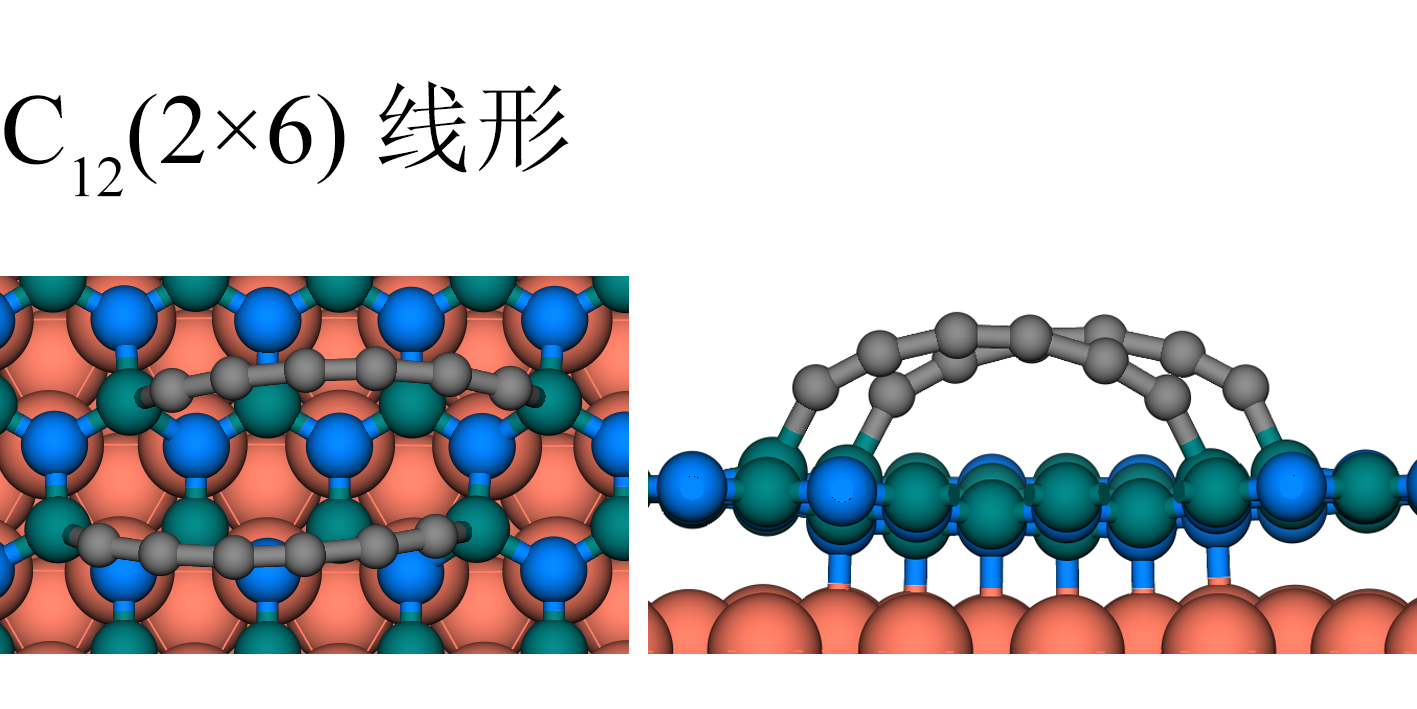
\includegraphics{pic/CG_structure_12C2L.png}
            \label{fig:CG_structure_12C2L}
        }
        \subfloat[]{
            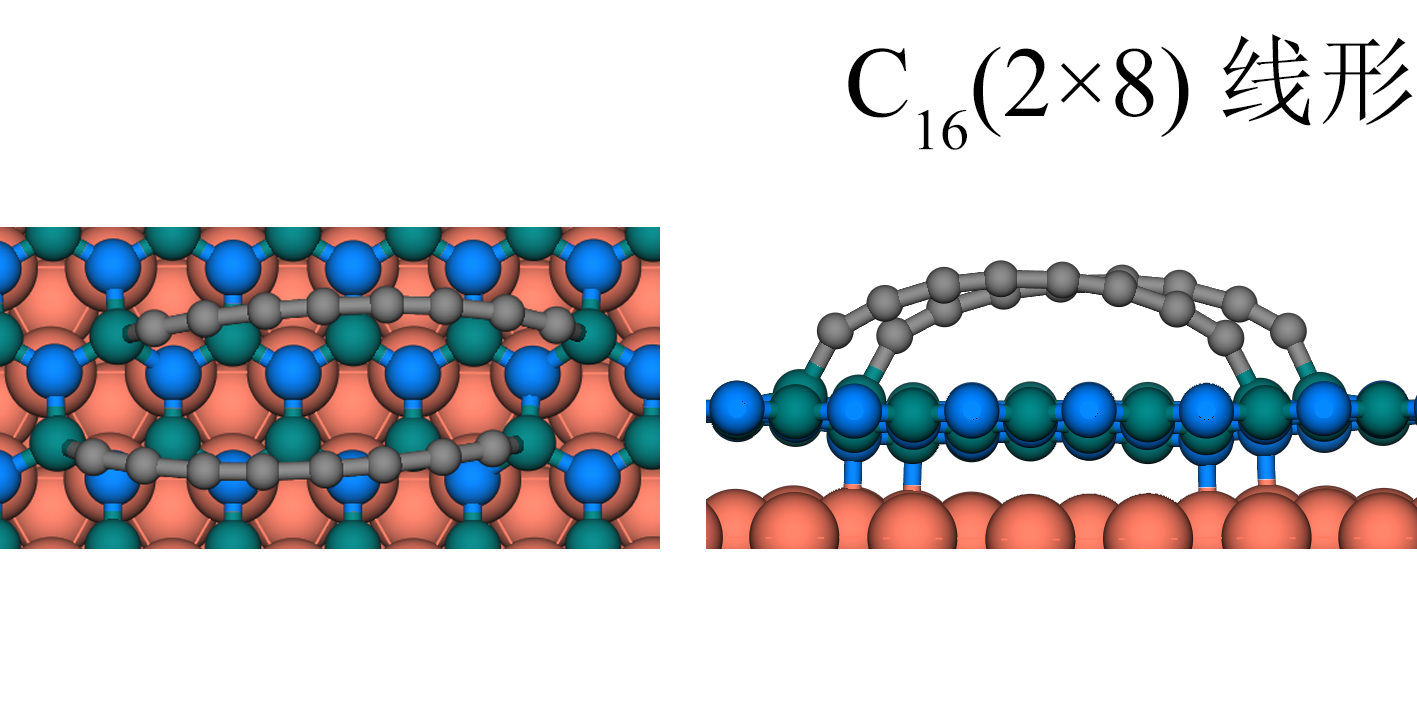
\includegraphics{pic/CG_structure_16C2L.png}
            \label{fig:CG_structure_16C2L}
        }
        \caption{游离\cemb{C}原子的扩散势垒以及\cemb{Cu/h-BN}表面\cemb{C}团簇的原子结构图。(a)\cemb{C}原子在\cemb{Cu/h-BN}表面的扩散势垒;(b)\cemb{C}原子在石墨烯/\cemb{h-BN}异质结表面的扩散势垒;(c)\cemb{C12}双线形团簇;(d)\cemb{C16}双线形团簇。原子结构图中,铜原子为橙色;氮原子为蓝色;硼原子为绿色;碳原子为灰色。}
        \label{}
    \end{figure}

    而对于线形的\cemb{C}团簇,由于其一维的原子结构,我们认为生长气氛中的\cemb{C}原子直接吸附至\cemb{C}线形团簇的表面参与生长的概率远低于平面结构的\cemb{C}六边形团簇和\cemb{C}环形团簇。因此\cemb{C}线形团簇的生长来源主要为在\cemb{h-BN}表面扩散的游离的\cemb{C}原子。在图\ref{pic:CG_DFT_CdiffonHBNCu}中,我们计算了游离的\cemb{C}原子在\cemb{h-BN}表面的扩散势垒。可以看到,由于\cemb{C}原子和\cemb{h-BN}表面非常强烈的相互作用,\cemb{C}原子在\cemb{h-BN}表面由\cemb{N}原子上方的吸附位点经过\cemb{B}原子到达相邻的等价吸附位点需要越过的势垒高度为\SI{2.39}{\electronvolt}。作为对比,我们计算了在覆盖在\cemb{Cu/h-BN}表面的石墨烯上游离的\cemb{C}原子的扩散势垒(图\ref{pic:CG_DFT_CdiffonGhBNCu}),用以模拟沉积的\cemb{C}原子在\cemb{C}六边形团簇上的扩散情况。在\cemb{h-BN}上石墨烯表面的\cemb{C}原子的扩散势垒为\SI{0.85}{\electronvolt},远低于\cemb{C}原子在\cemb{h-BN}表面的扩散势垒。

    因此我们认为对于\cemb{C}线形团簇而言,由于受到\cemb{C}原子高迁移势垒的限制,单个\cemb{C}线形团簇难以在实际的成核生长过程中生长到非常长的情况,而是近邻的\cemb{C}原子相结合,形成多条短的\cemb{C}线形团簇(图\ref{fig:CG_structure_12C2L}和图\ref{fig:CG_structure_16C2L})。当\cemb{C}线形团簇由于\cemb{C}原子高迁移势垒而受困于以多条短线组成的\cemb{C}团簇暂稳态后,\cemb{C}线形团簇的平均\cemb{C}原子形成能开始缓慢上升。以6个\cemb{C}原子线形团簇为基元的\cemb{C12}$\left(2 \times 6\right)$线形团簇和\cemb{C18}$\left(3 \times 6\right)$线形团簇的平均\cemb{C}原子形成能为\SI{-6.63}{\electronvolt\per\atom}和\SI{-6.59}{\electronvolt\per\atom}。以8个\cemb{C}原子线形团簇为基元的双线(\cemb{C16}$\left(2 \times 8\right)$,图\ref{fig:CG_structure_16C2L})、三线形团簇(\cemb{C24}$\left(3 \times 8\right)$)的形成能也略高于\cemb{C8}线形团簇的能量。

    \begin{figure}[htb]
        \subfloat[]{
            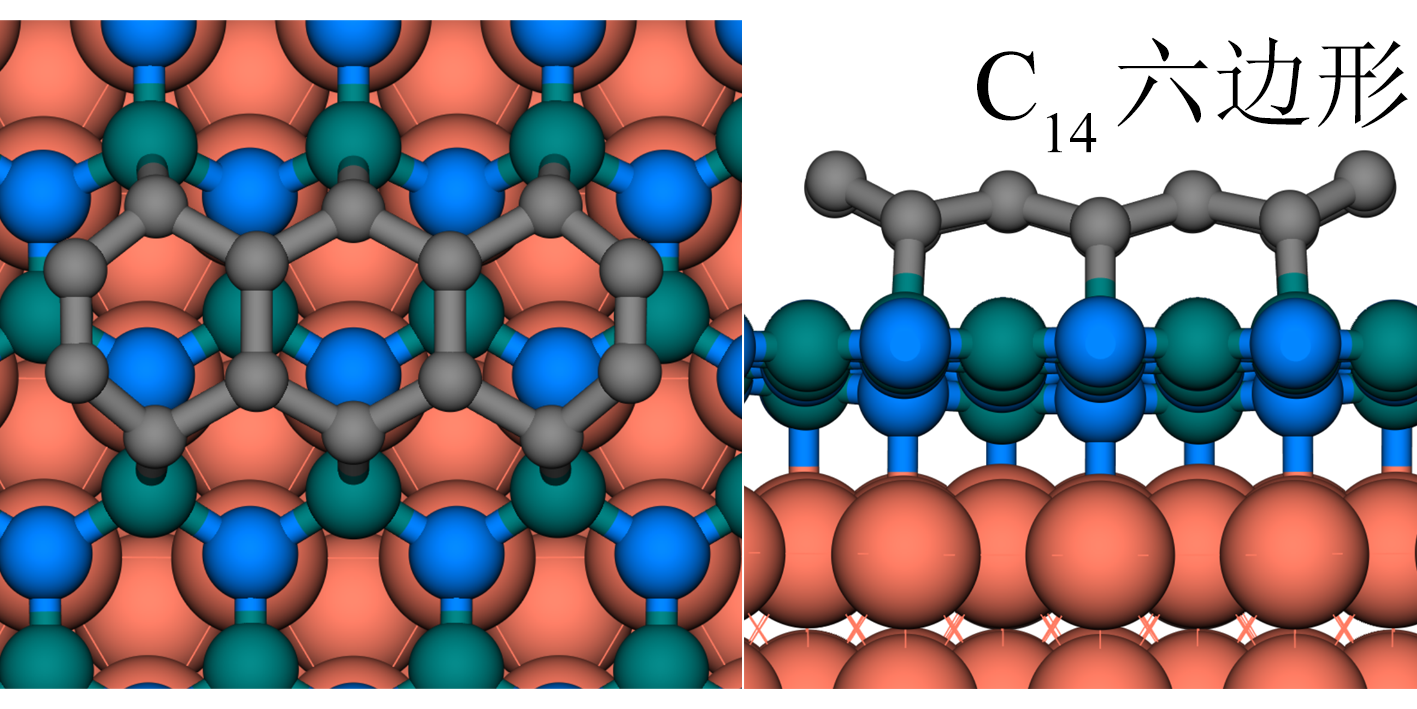
\includegraphics{pic/CG_structure_14CH.png}
            \label{fig:CG_structure_14CH}
        }
        \subfloat[]{
            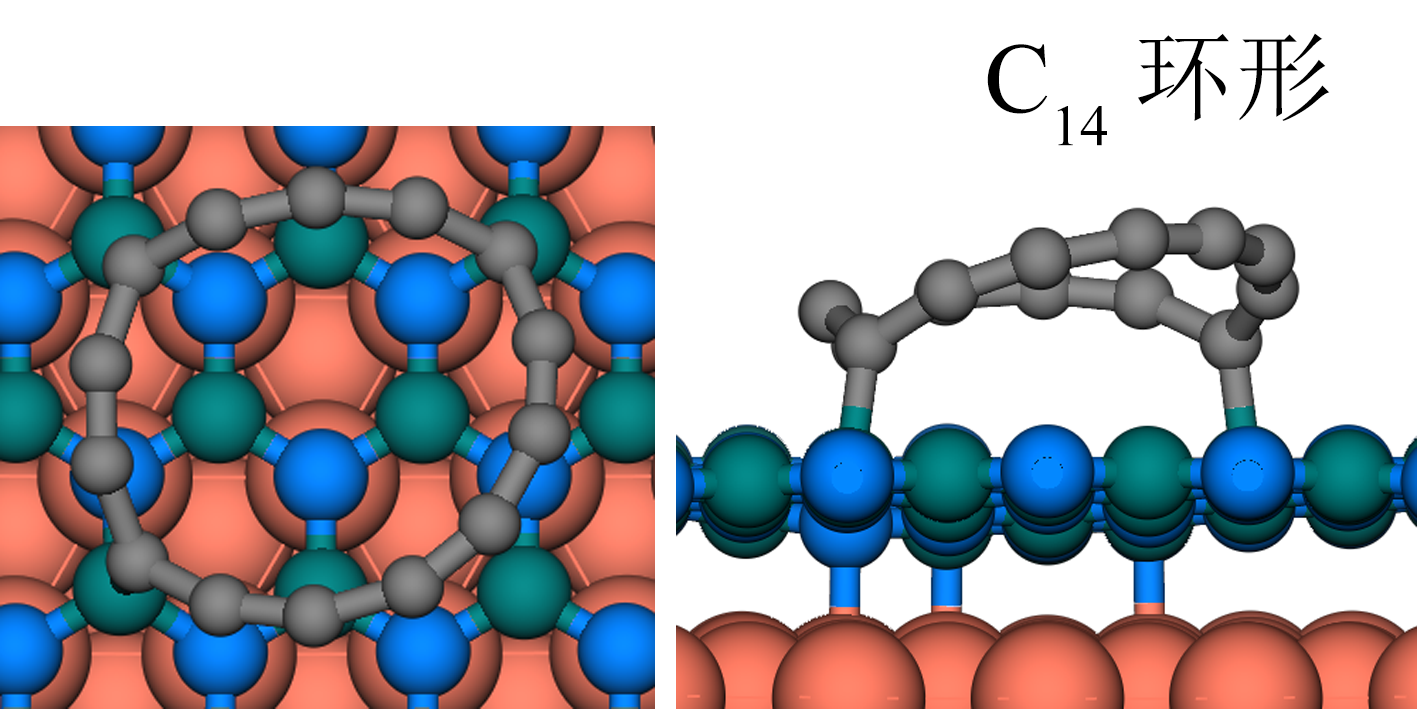
\includegraphics{pic/CG_structure_14CR.png}
            \label{fig:CG_structure_14CR}
        }
        \\[-0.5ex]
        \subfloat[]{
            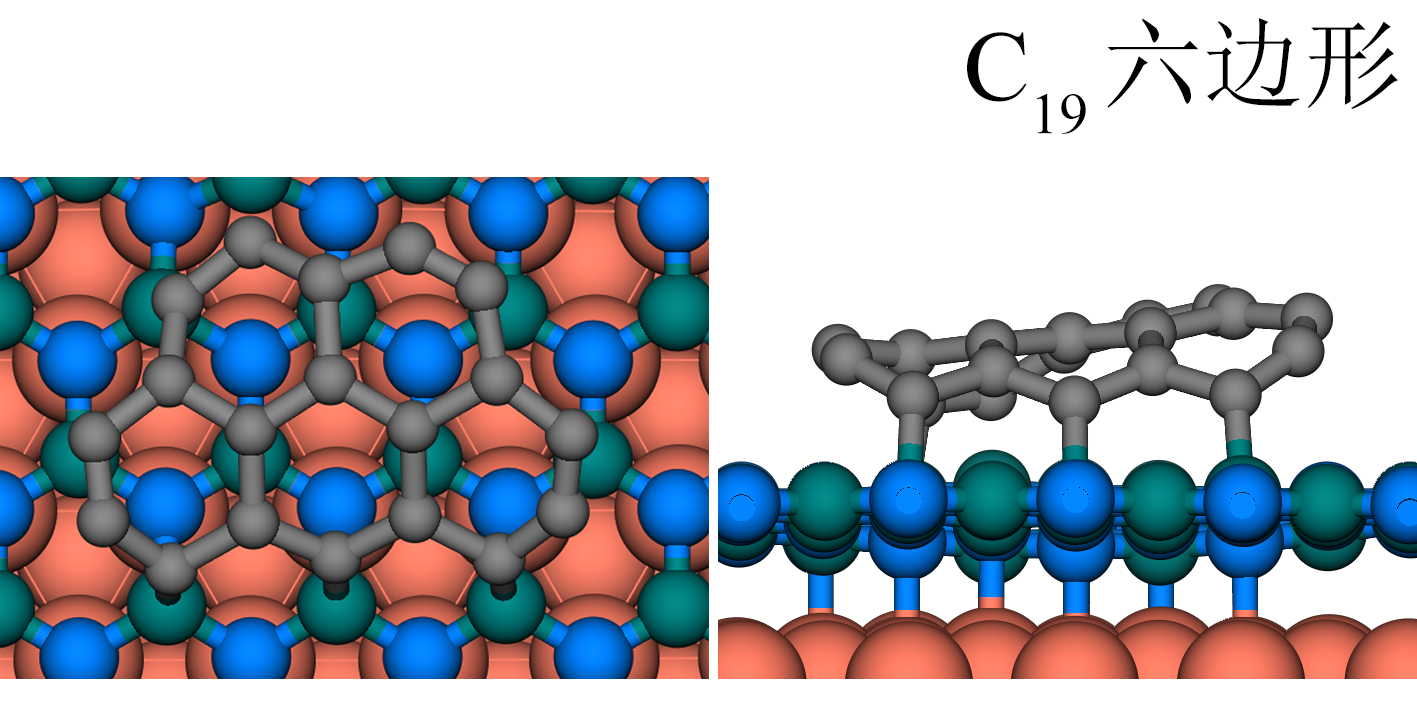
\includegraphics{pic/CG_structure_19CH.png}
        }
        \subfloat[]{
            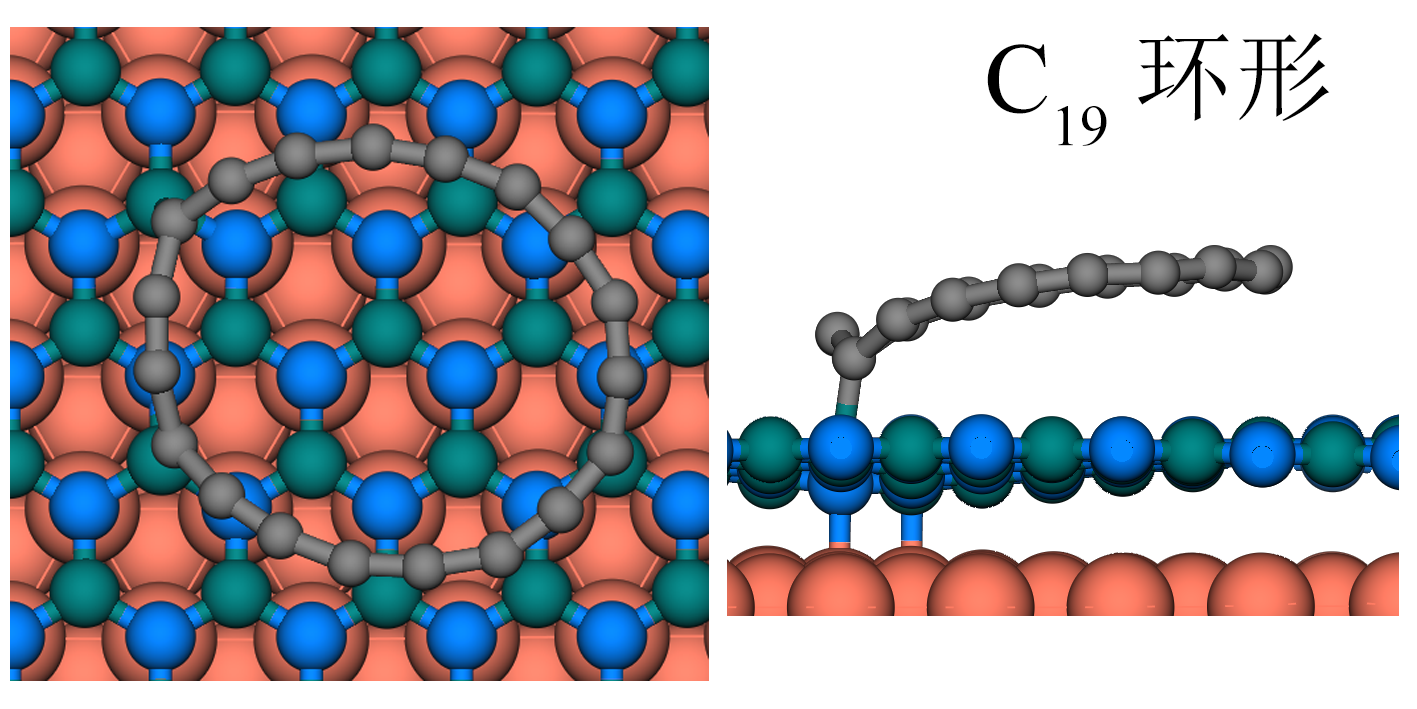
\includegraphics{pic/CG_structure_19CR.png}
        }
        \caption{\cemb{Cu/h-BN}表面\cemb{C}团簇的原子结构图。(a)\cemb{C4}六边形团簇;(b)\cemb{14}环形团簇;(c)\cemb{C19}六边形团簇;(d)\cemb{C19}环形团簇。原子结构图中,铜原子为橙色;氮原子为蓝色;硼原子为绿色;碳原子为灰色。}
        \label{fig:CG_CG_structure_14-19C}
    \end{figure}
    
    当\cemb{C}团簇中的\cemb{C}原子数量上升到14个,14个\cemb{C}原子能够在\cemb{h-BN}的表面形成三个六元环(\cemb{C14}六边形团簇,图\ref{fig:CG_structure_14CH})。\cemb{C14}六边形团簇的平均\cemb{C}原子形成能(\SI{-6.74}{\electronvolt\per\atom})略高于将六元环内部相邻的sp2杂化\cemb{C}原子的连接打开,形成\cemb{C14}环形团簇的形成能(\SI{-6.85}{\electronvolt\per\atom})。在\cemb{C14}环形团簇中,有3个\cemb{C}原子与\cemb{h-BN}表面的\cemb{B}原子成键,恰好对应于\cemb{h-BN}上次近邻\cemb{B}原子所组成的矩形的三个顶角原子。

    \cemb{C}六边形团簇形成能高于环形团簇的情况在团簇内\cemb{C}原子数量到达19个时发生了逆转。\cemb{C19}六边形团簇的平均\cemb{C}原子结合能(\SI{-6.98}{\electronvolt\per\atom})低于\cemb{19}环形团簇的结合能(\SI{-6.94}{\electronvolt\per\atom})。在\cemb{C19}六边形团簇中,19个\cemb{C}原子形成了5个六元环。\cemb{h-BN}衬底表面的\cemb{B}原子只能束缚住其中4个六元环,有1个六元环由于六边形团簇平面内应力释放的原因脱离了\cemb{B}原子的吸引,减小了\cemb{C19}六边形团簇整体的弯曲程度。同样,对于\cemb{C19}环形团簇,在优化后的结构中,有一半以上的\cemb{C}原子脱离了\cemb{h-BN}的束缚,在真空中尽可能的延展以接近理想的sp杂化\cemb{C}的直线构型。

    \begin{figure}[htb]
        \subfloat[]{
            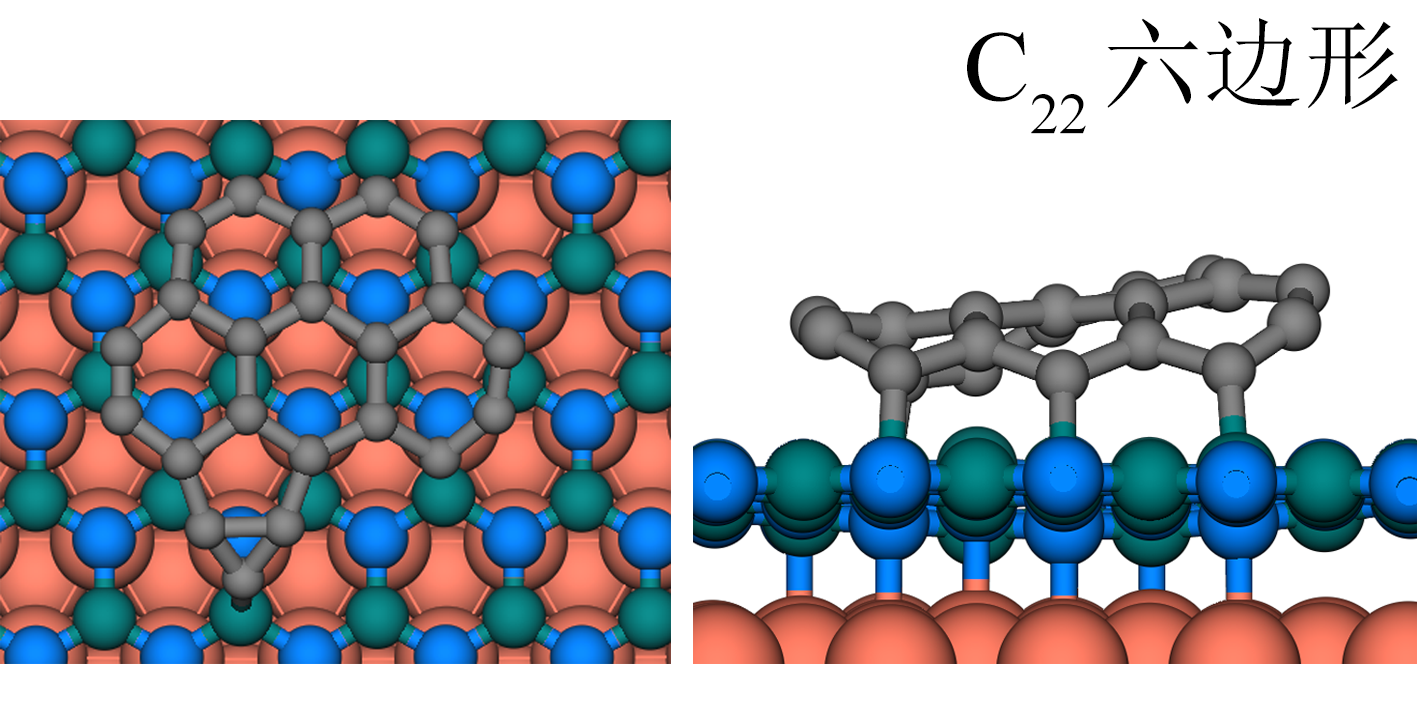
\includegraphics{pic/CG_structure_22CH.png}
            \label{fig:CG_structure_22CH}
        }
        \subfloat[]{
            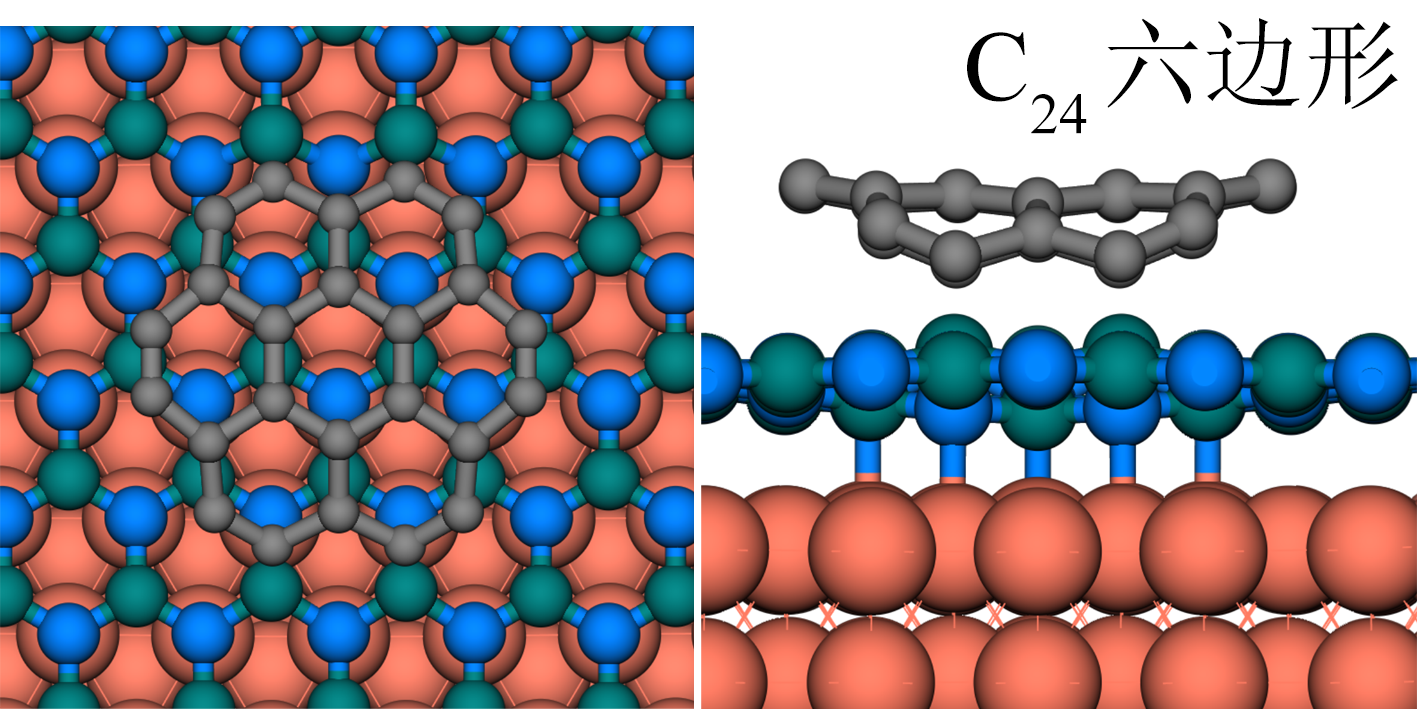
\includegraphics{pic/CG_structure_24CH.png}
            \label{fig:CG_structure_24CH}
        }
        \caption{\cemb{Cu/h-BN}表面\cemb{C}团簇的原子结构图。(a)\cemb{C22}六边形团簇;(b)\cemb{24}六边形团簇。原子结构图中,铜原子为橙色;氮原子为蓝色;硼原子为绿色;碳原子为灰色。}
        \label{fig:CG_CG_structure_22-24C}
    \end{figure}

    随着更多的\cemb{C}原子附着在\cemb{C}团簇上,\cemb{C}团簇生长为包含5个\cemb{C}六元环的\cemb{C22}六边形团簇(\ref{fig:CG_structure_22CH})和包含6个\cemb{C}六元环的\cemb{C24}六边形团簇(\ref{fig:CG_structure_22CH})。这些在六边形团簇中,与\cemb{h-BN}表面具有明显相互作用的均为锯齿边缘的\cemb{C}原子,而扶手椅边缘的\cemb{C}原子则向上翘起对六边形团簇内sp2杂化\cemb{C}原子的平面内应力进行释放。
    
    同时,我们可以发现,在\cemb{h-BN}表面与\cemb{C}团簇边缘原子产生相互作用的基本为\cemb{B}原子。在石墨烯生长的初期阶段,\cemb{C}原子组成的团簇首先倾向于形成以sp杂化\cemb{C}为主要组成的线形的团簇。但由于沉积的\cemb{C}原子在\cemb{h-BN}表面迁移困难,当形成\cemb{C}团簇的原子数上升到十几个\cemb{C}原子时,\cemb{C}团簇倾向于呈现出环形的相貌。由于sp2杂化\cemb{C}在原子数较少的\cemb{C}团簇内形成能的相对弱势,只有当\cemb{C}团簇内的\cemb{C}原子大于19个时,\cemb{C}团簇才会倾向于将结构演化为以\cemb{C}六元环为基本单元的\cemb{C}六边形团簇,从而实现同样以\cemb{C}六元环为基本单元的石墨烯在\cemb{Cu/h-BN}表面的生长。

\section{石墨烯/\cemb{VSe2}横向异质结的生长机理}
    \subsection{石墨烯表面\cemb{V}原子、\cemb{Se}原子的吸附机理}
    \label{cap:VS}
    对于石墨烯/\cemb{VSe2}的生长,我们首先利用密度泛函理论计算了\cemb{V}原子和\cemb{Se}原子在石墨烯表面的吸附情况。如图\ref{fig:VS_VandSeOnG}所示,\cemb{V}原子在石墨烯表面的最佳吸附位点为\cemb{C}六元环的中央空位。吸附后,\cemb{V}原子略微偏离六元环的中央空位位点,此时\cemb{V-C}键的键长约为\SIrange[range-phrase=$\sim$]{2.27}{2.40}{\angstrom}。而对于\cemb{Se}原子,其在石墨烯表面的最佳吸附位点为\cemb{C}六元环边缘的桥位。此时,\cemb{Se}原子与相邻的两个\cemb{C}原子成键,键长为\SI{2.14}{\angstrom}。

    \begin{figure}[htb]
        \subfloat[]{
            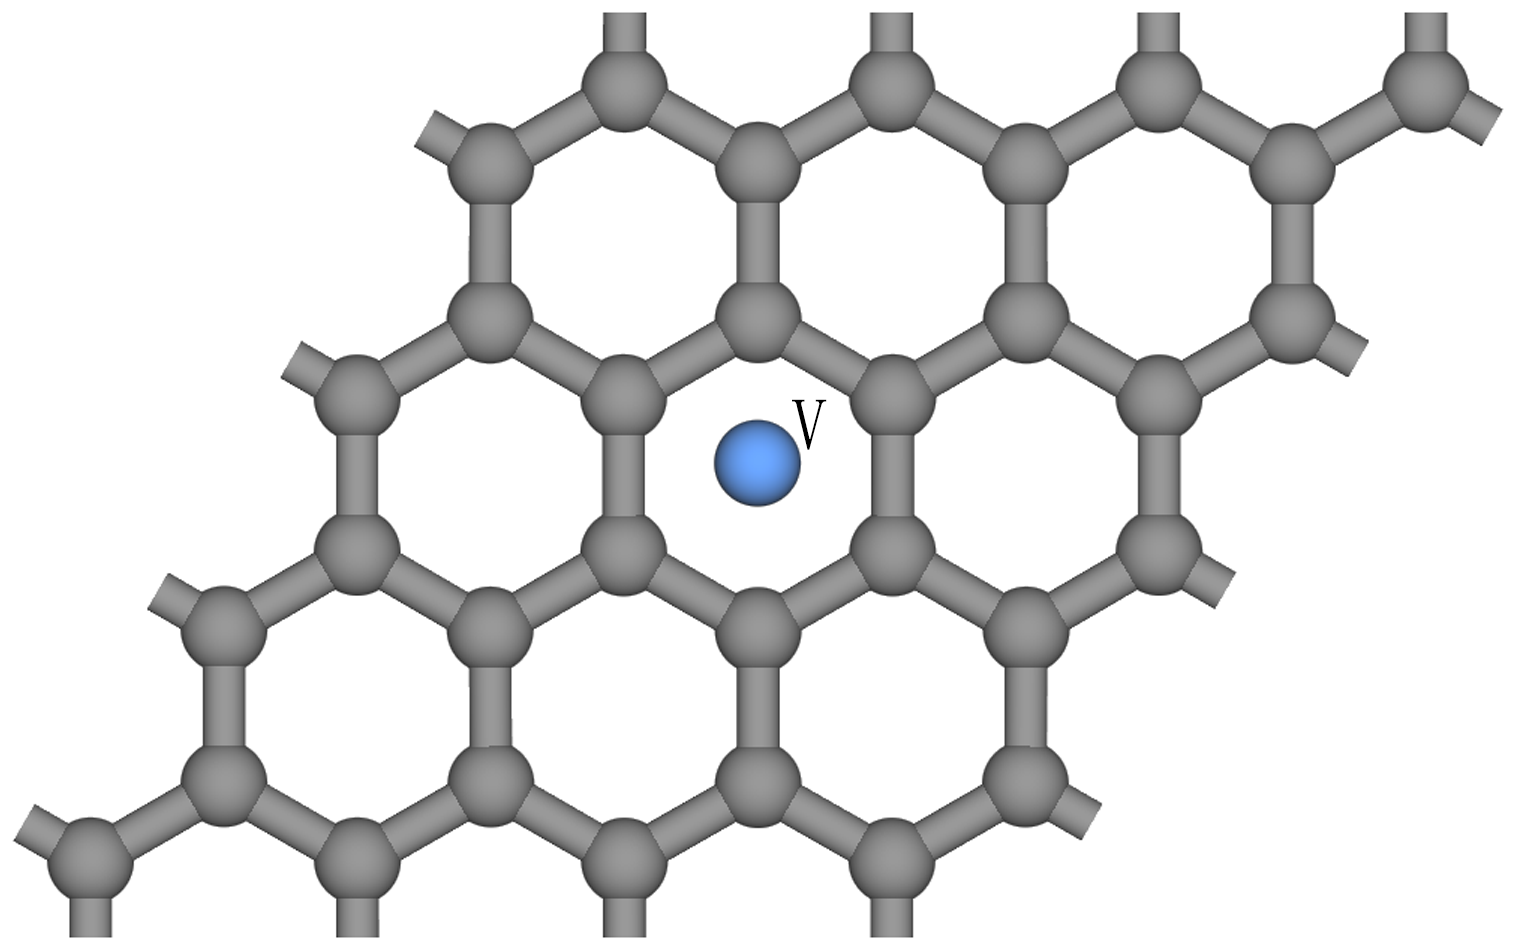
\includegraphics{pic/VS_structure_VOnG.png}
        }
        \subfloat[]{
            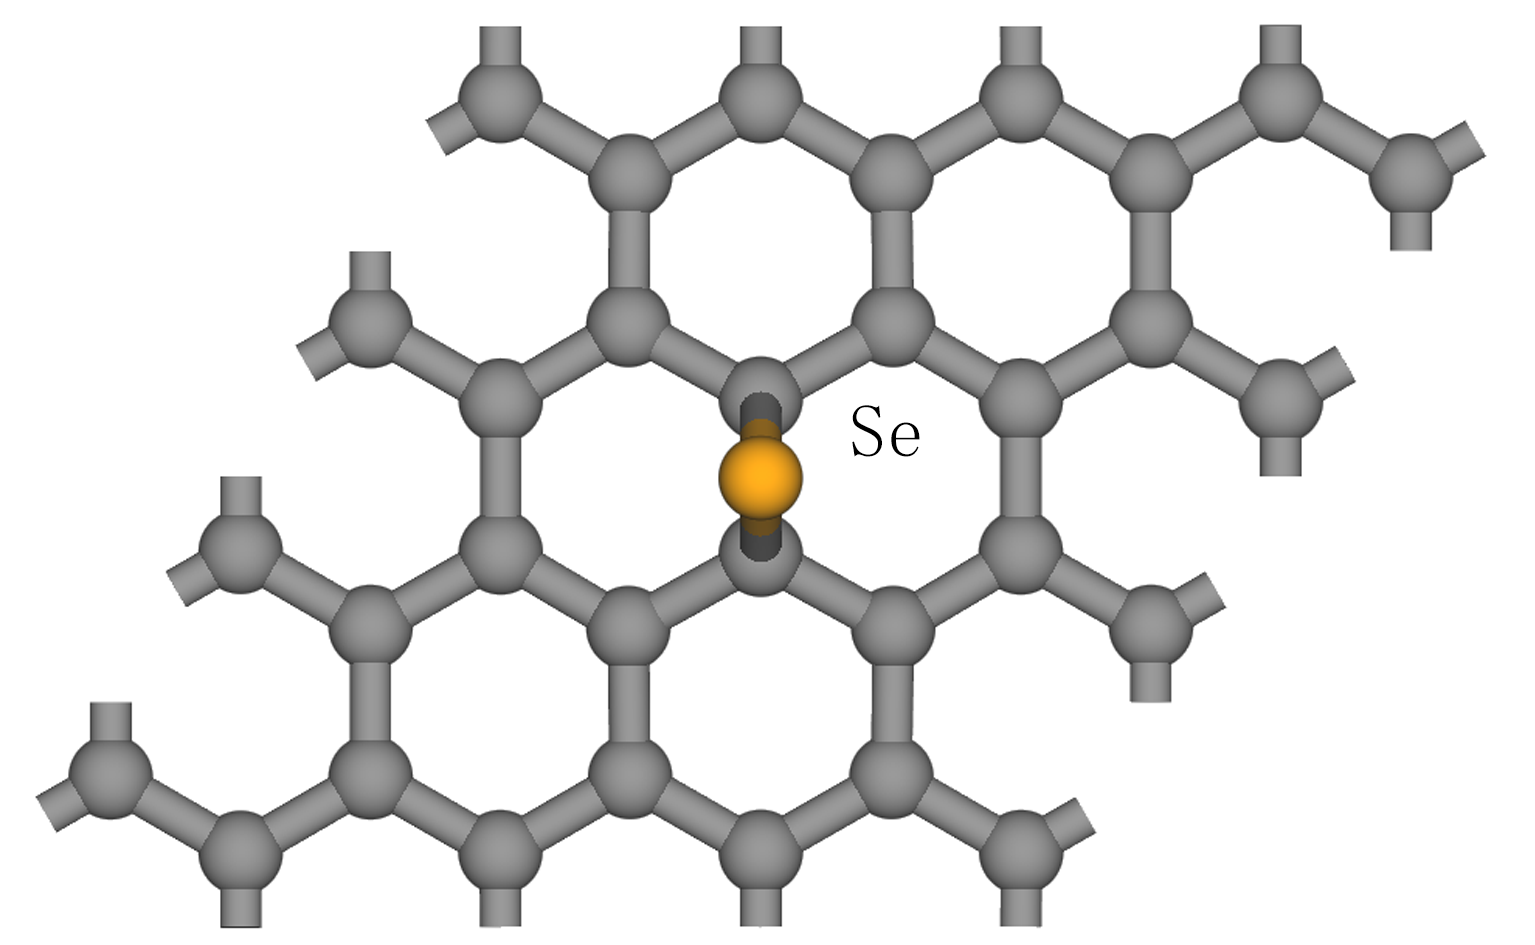
\includegraphics{pic/VS_structure_SeOnG.png}
        }
        \caption{\cemb{V}原子和\cemb{Se}原子在石墨烯表面的最优吸附位点。(a)\cemb{V}原子在石墨烯表面吸附;(b)\cemb{Se}原子在石墨烯表面吸附。在原子结构图中,钒原子为蓝色;碳原子为灰色;硒原子为橙色。}
        \label{fig:VS_VandSeOnG}
    \end{figure}

    在石墨烯的表面,吸附原子的结合能$\energyVar{b}{}$可以用来表征不同原子吸附能力的强弱\chinesecolon
    \[
        \energyVar{b}{}=\left(\energyVar{sub+adatom}{}-\energyVar{sub}{}-N\muVar{adatom}{}\right)/ N
    \]
    其中,$\energyVar{sub+adatom}{}$和$\energyVar{sub}{}$为吸附有原子的衬底和未吸附原子的衬底的能量。$\muVar{adatom}{}$为吸附原子的化学势。$N$为吸附原子的总数。

    对于$\muVar{adatom}{}$为吸附原子的化学势,我们首先考虑于生长环境下\cemb{VSe2}块体的化学平衡,我们有\chinesecolon
    \begin{equation}
        \label{eq:VS_bulkEqmb}
        \muVar{V}{}+2\muVar{Se}{}=\energyVar{\ce{VSe2}}{tot}=\energyVar{V\left(Bulk\right)}{}+2\energyVar{Se\left(Bulk\right)}{}+\rm{\Delta} \it H_{\rm f}\left(\ce{VSe2}\right)
    \end{equation}
    其中,$\energyVar{\ce{VSe2}}{tot}$、$\energyVar{V\left(Bulk\right)}{}$和$\energyVar{Se\left(Bulk\right)}{}$为\cemb{VSe2}块体,\cemb{V}块体和\cemb{Se}块体的能量。因此,在\cemb{VSe2}块体的化学平衡的限制下,$\muVar{V}{}$的变化范围为$\energyVar{V\left(Bulk\right)}{}+\rm{\Delta} \it H_{\rm f}\left(\ce{VSe2}\right) \leqslant \muVar{V}{}  \leqslant \energyVar{V\left(Bulk\right)}{}$,代表\cemb{V}的化学势$\muVar{V}{}$由纯\cemb{Se}的生长环境变化到纯\cemb{V}的生长环境。

    在图\ref{fig:VS_DFT_adatoms}中,我们计算了\cemb{V}原子和\cemb{Se}原子在石墨烯对应的最优吸附位点的吸附能随化学势$\muVar{V}{}$的变化情况。可以看到,对于\cemb{V}原子和\cemb{Se}原子,在\cemb{VSe2}块体平衡的限制下均无法在石墨烯表面自发吸附。对于\cemb{V}原子,在纯\cemb{V}的极限环境下,从生长气氛中裂解,吸附到石墨烯表面所需要吸收的能量为\SI{4.48}{\electronvolt}。而在纯\cemb{Se}的极限环境下,\cemb{V}原子从裂解到吸附在石墨烯表面需要吸收的能量为\SI{6.38}{\electronvolt}。\cemb{Se}原子在\cemb{VSe2}块体平衡的限制下的吸附能力强于\cemb{V}原子。在纯\cemb{V}的极限环境下,\cemb{Se}原子从生长气环境中裂解,吸附在石墨烯的表面只需要消耗\SI{2.32}{\electronvolt}的能量。而在纯\cemb{V}的极限环境下,生长气氛中的\cemb{Se}原子吸附在石墨烯的表面所吸收的能量只上升至\SI{3.27}{\electronvolt},低于此环境下\cemb{V}原子在石墨烯表面的结合能。

    \begin{figure}[htb]
        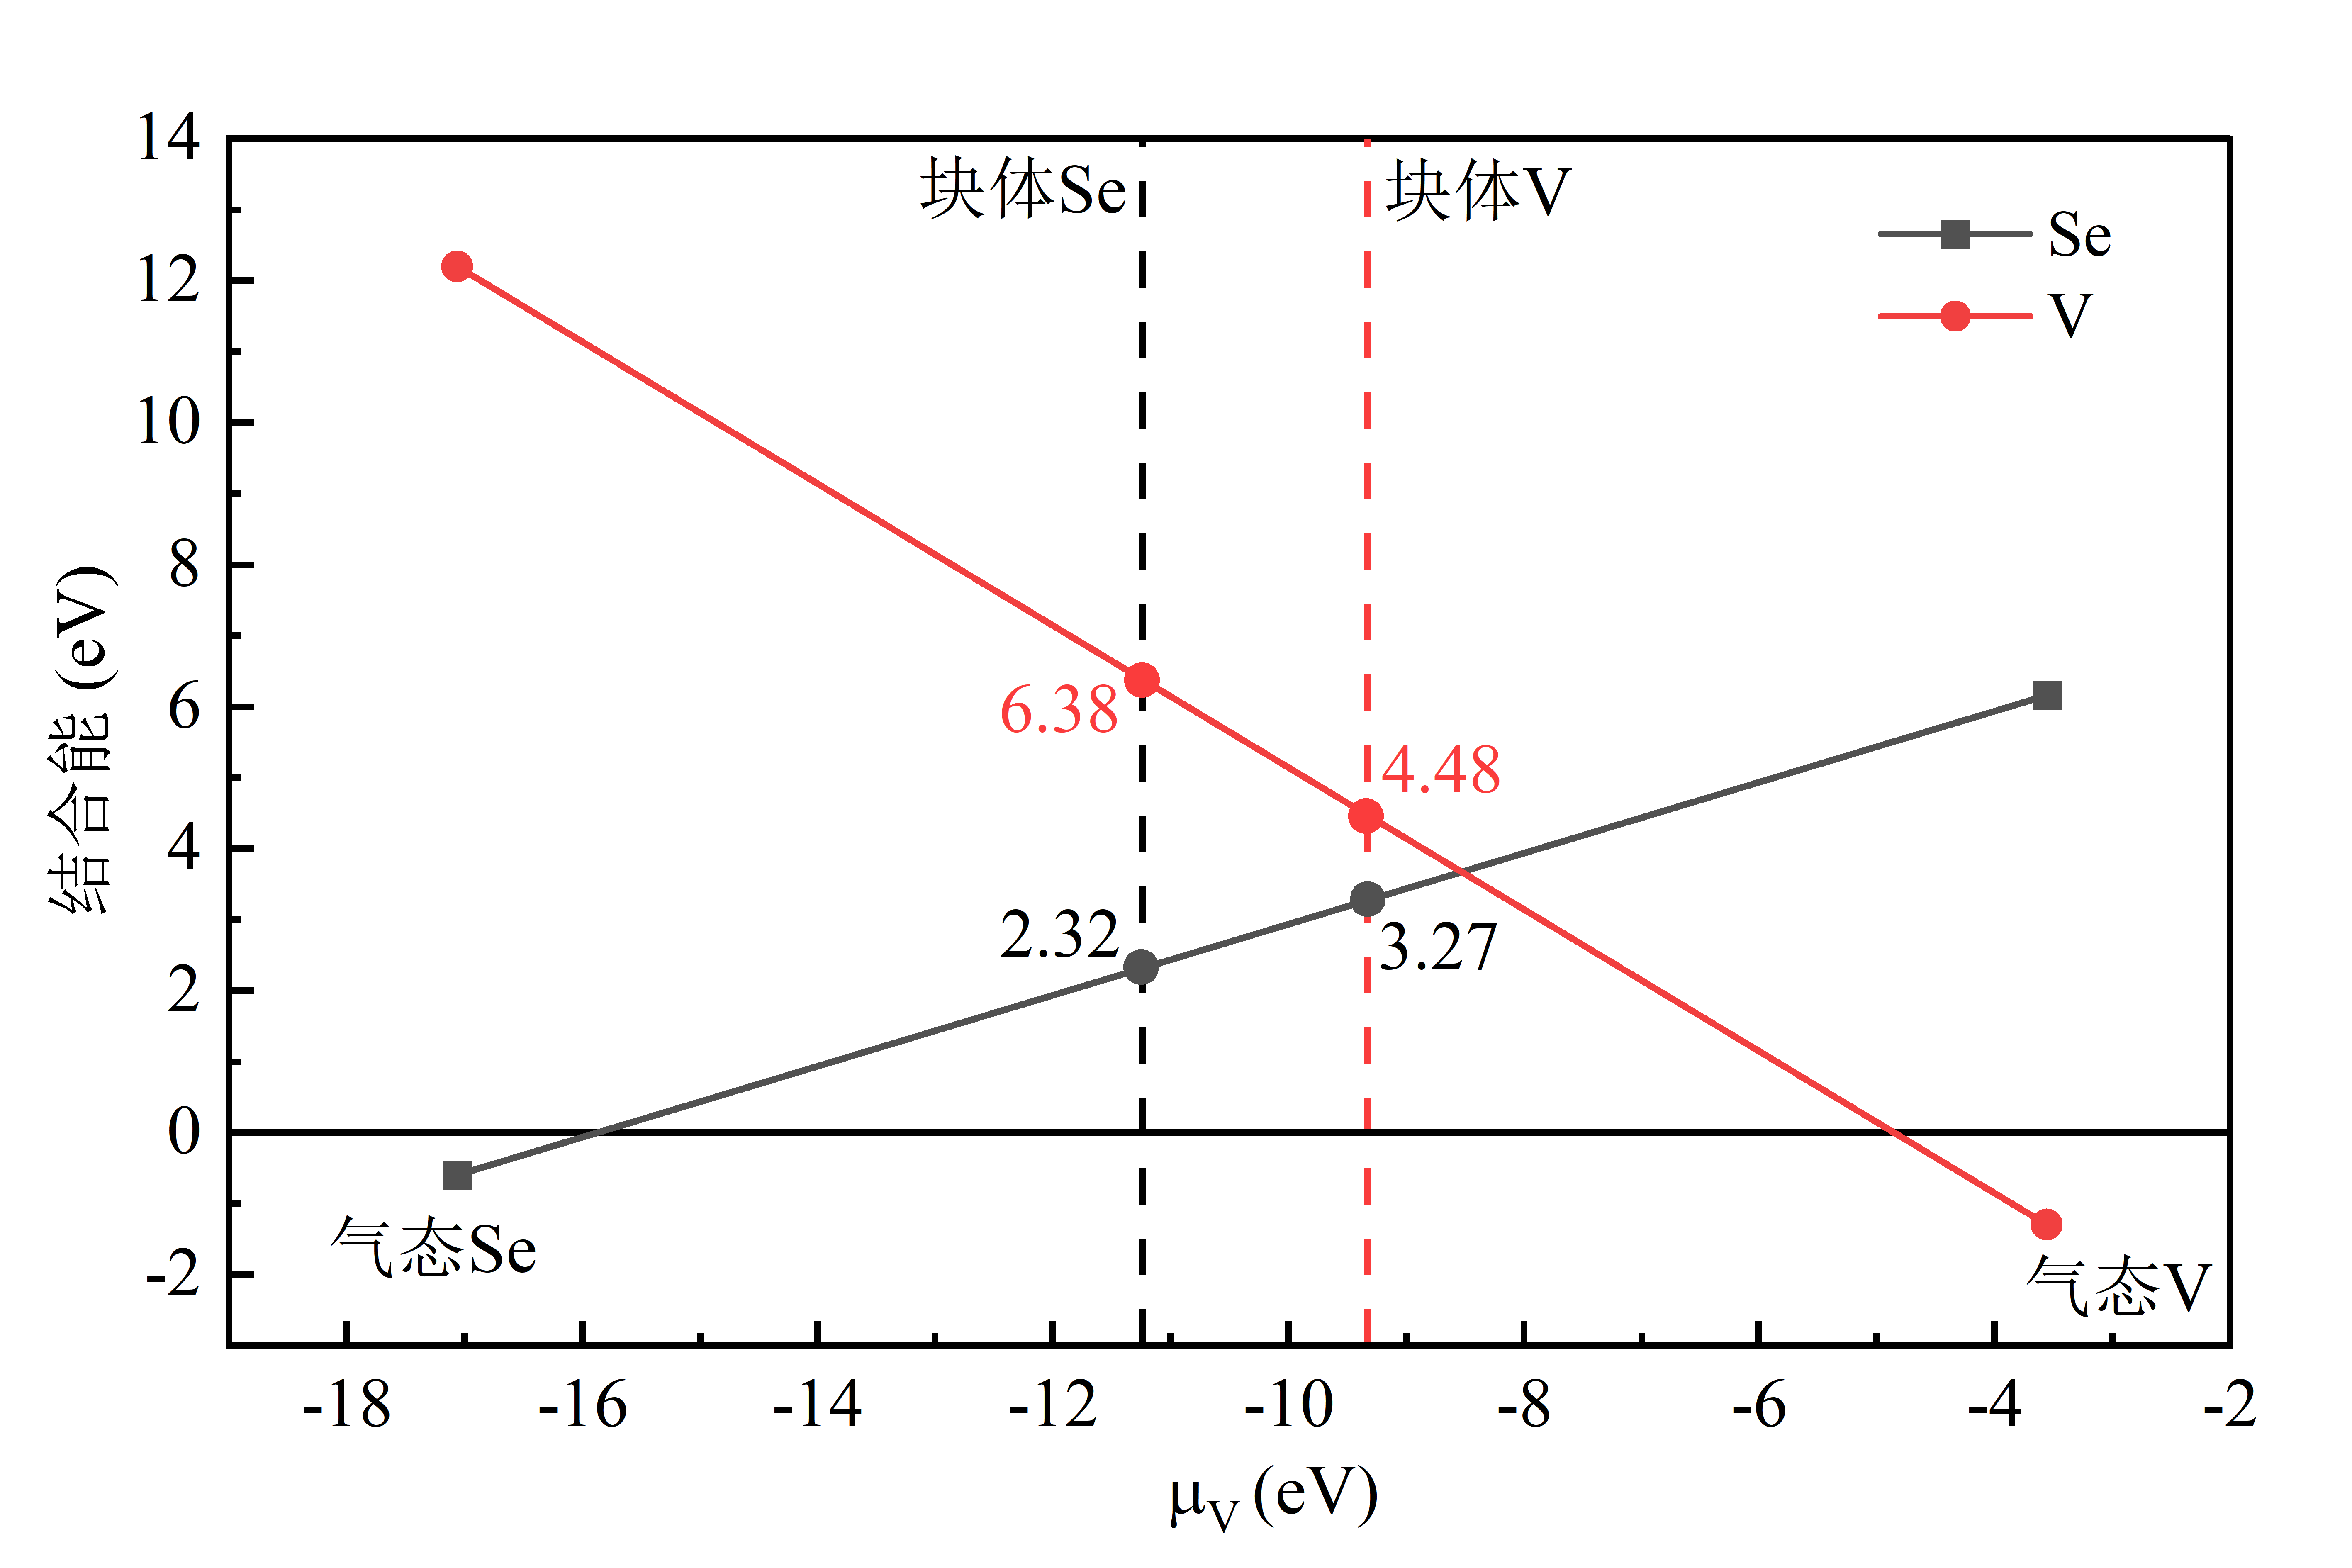
\includegraphics{pic/VS_DFT_adatoms.png}
        \caption{石墨烯表面\cemb{V}原子和\cemb{Se}原子的吸附能随化学势$\muVar{V}{}$的变化情况}
        \label{fig:VS_DFT_adatoms}
    \end{figure}

    而要使\cemb{V}原子和\cemb{Se}原子能够自发的在石墨烯的表面吸附,为\cemb{VSe2}的生长提供物质来源,需要进一步提高生长环境中气态分子的能量,使得前驱体\cemb{VSe2}在气相的状态下分解为包含\cemb{Se}原子和\cemb{V}原子的自由基,突破\cemb{VSe2}块体的化学平衡的限制。为了考虑更高活性的\cemb{V}原子和\cemb{Se}原子在石墨烯表面的吸附情况,我们将$\muVar{V}{}$的取值范围扩展到气态\cemb{Se}原子和气态\cemb{V}原子环境中的能级水平。可以看到对于气态的\cemb{V}原子,其在石墨烯表面吸附的结合能为\SI{-1.30}{\electronvolt},略高于气态的\cemb{Se}原子在石墨烯表面吸附的结合能(\SI{-0.59}{\electronvolt})。在气态的状态下,\cemb{V}原子和\cemb{Se}原子均可在石墨烯的表面自发吸附。因此如果需要在石墨烯的表面生长\cemb{VSe2},生长环境需要提供足够高的温度使得气相中的\cemb{VSe2}得以裂解为活性的气态\cemb{V}自由基和气态\cemb{Se}自由基。

\subsection{石墨烯/\cemb{VSe2}的横向二维异质结的生长机理}
    在石墨烯台阶的边缘直接生长\cemb{VSe2}可形成石墨烯/\cemb{VSe2}横向异质结。在石墨烯/\cemb{VSe2}横向异质结中,石墨烯边缘的\cemb{C}原子和\cemb{VSe2}边缘的\cemb{V}原子或者\cemb{Se}原子成键。在本章中,我们关注具有与自然形成的块体\cemb{VSe2}具有相似原子层结构的1T相单层\cemb{VSe2}在石墨烯台阶不同边缘(扶手椅边缘和锯齿边缘)的生长。与石墨烯类似,\cemb{VSe2}也有扶手椅和锯齿两种不同的边缘。对于扶手椅边缘的\cemb{VSe2},其边缘由空悬的\cemb{V}原子和\cemb{Se}原子共同组成。对于锯齿边缘的\cemb{VSe2},我们在本章中先关注具有\cemb{Se}空悬原子的边缘构型。由于相似的边缘晶格构型,我们将石墨烯和\cemb{VSe2}之间的边界线匹配限制在同种边缘之间。也就是石墨烯扶手椅边缘匹配\cemb{VSe2}扶手椅边缘,而石墨烯锯齿边缘匹配\cemb{VSe2}锯齿边缘。

    \begin{figure}[htb]
        \subfloat[]{
            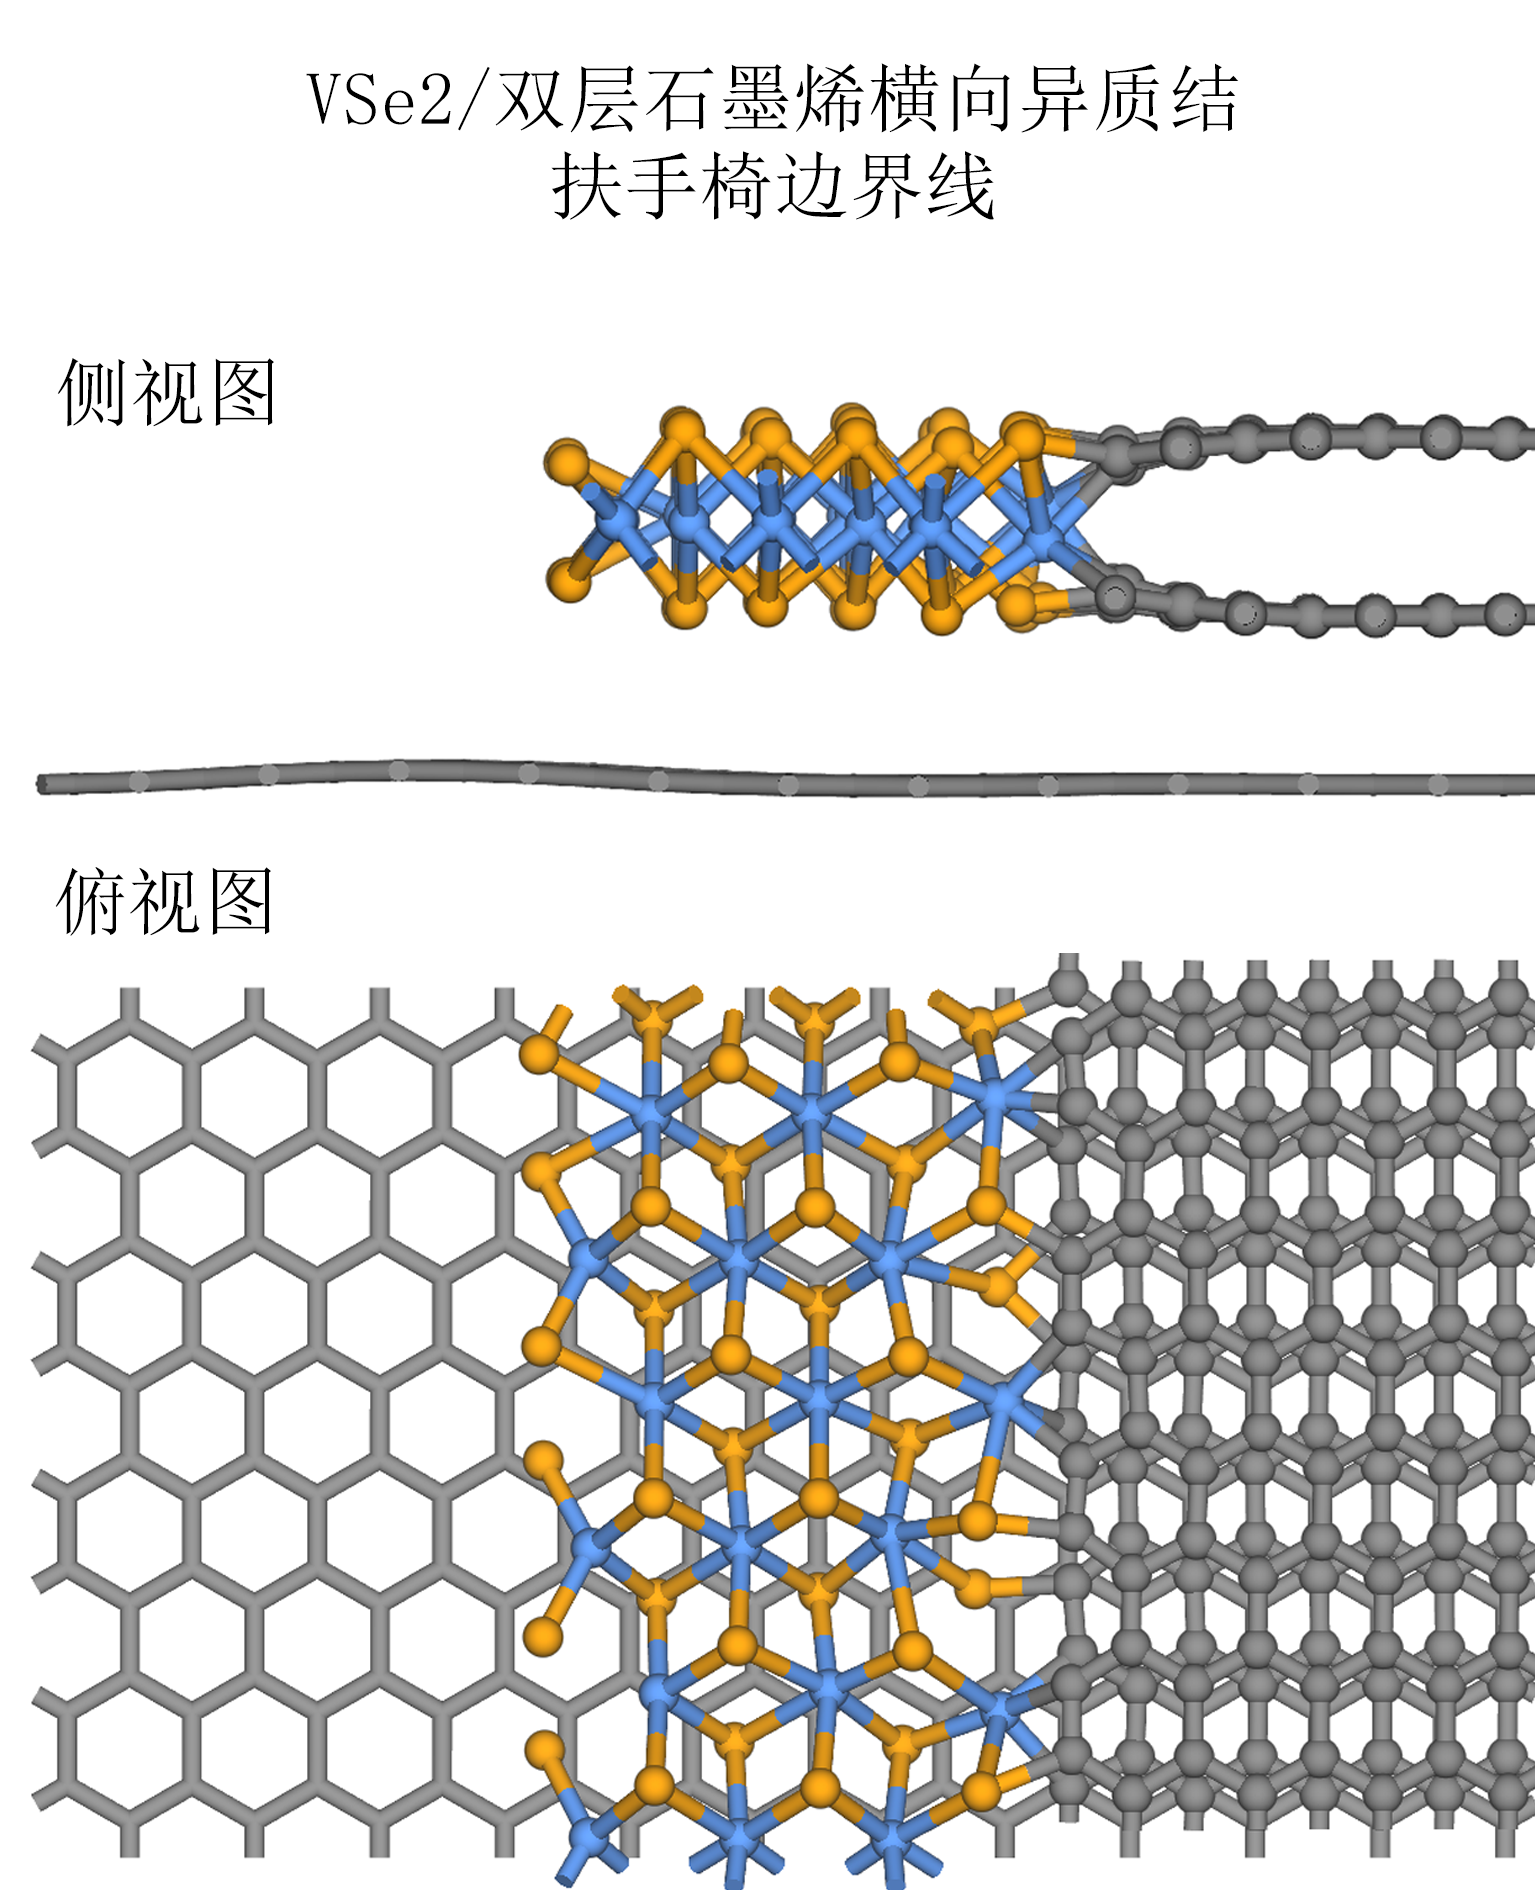
\includegraphics{pic/VS_structure_armchair_VSe2-2SG.png}
            \label{fig:VS_structure_armchair_VSe2-2SG}
        }
        \subfloat[]{
            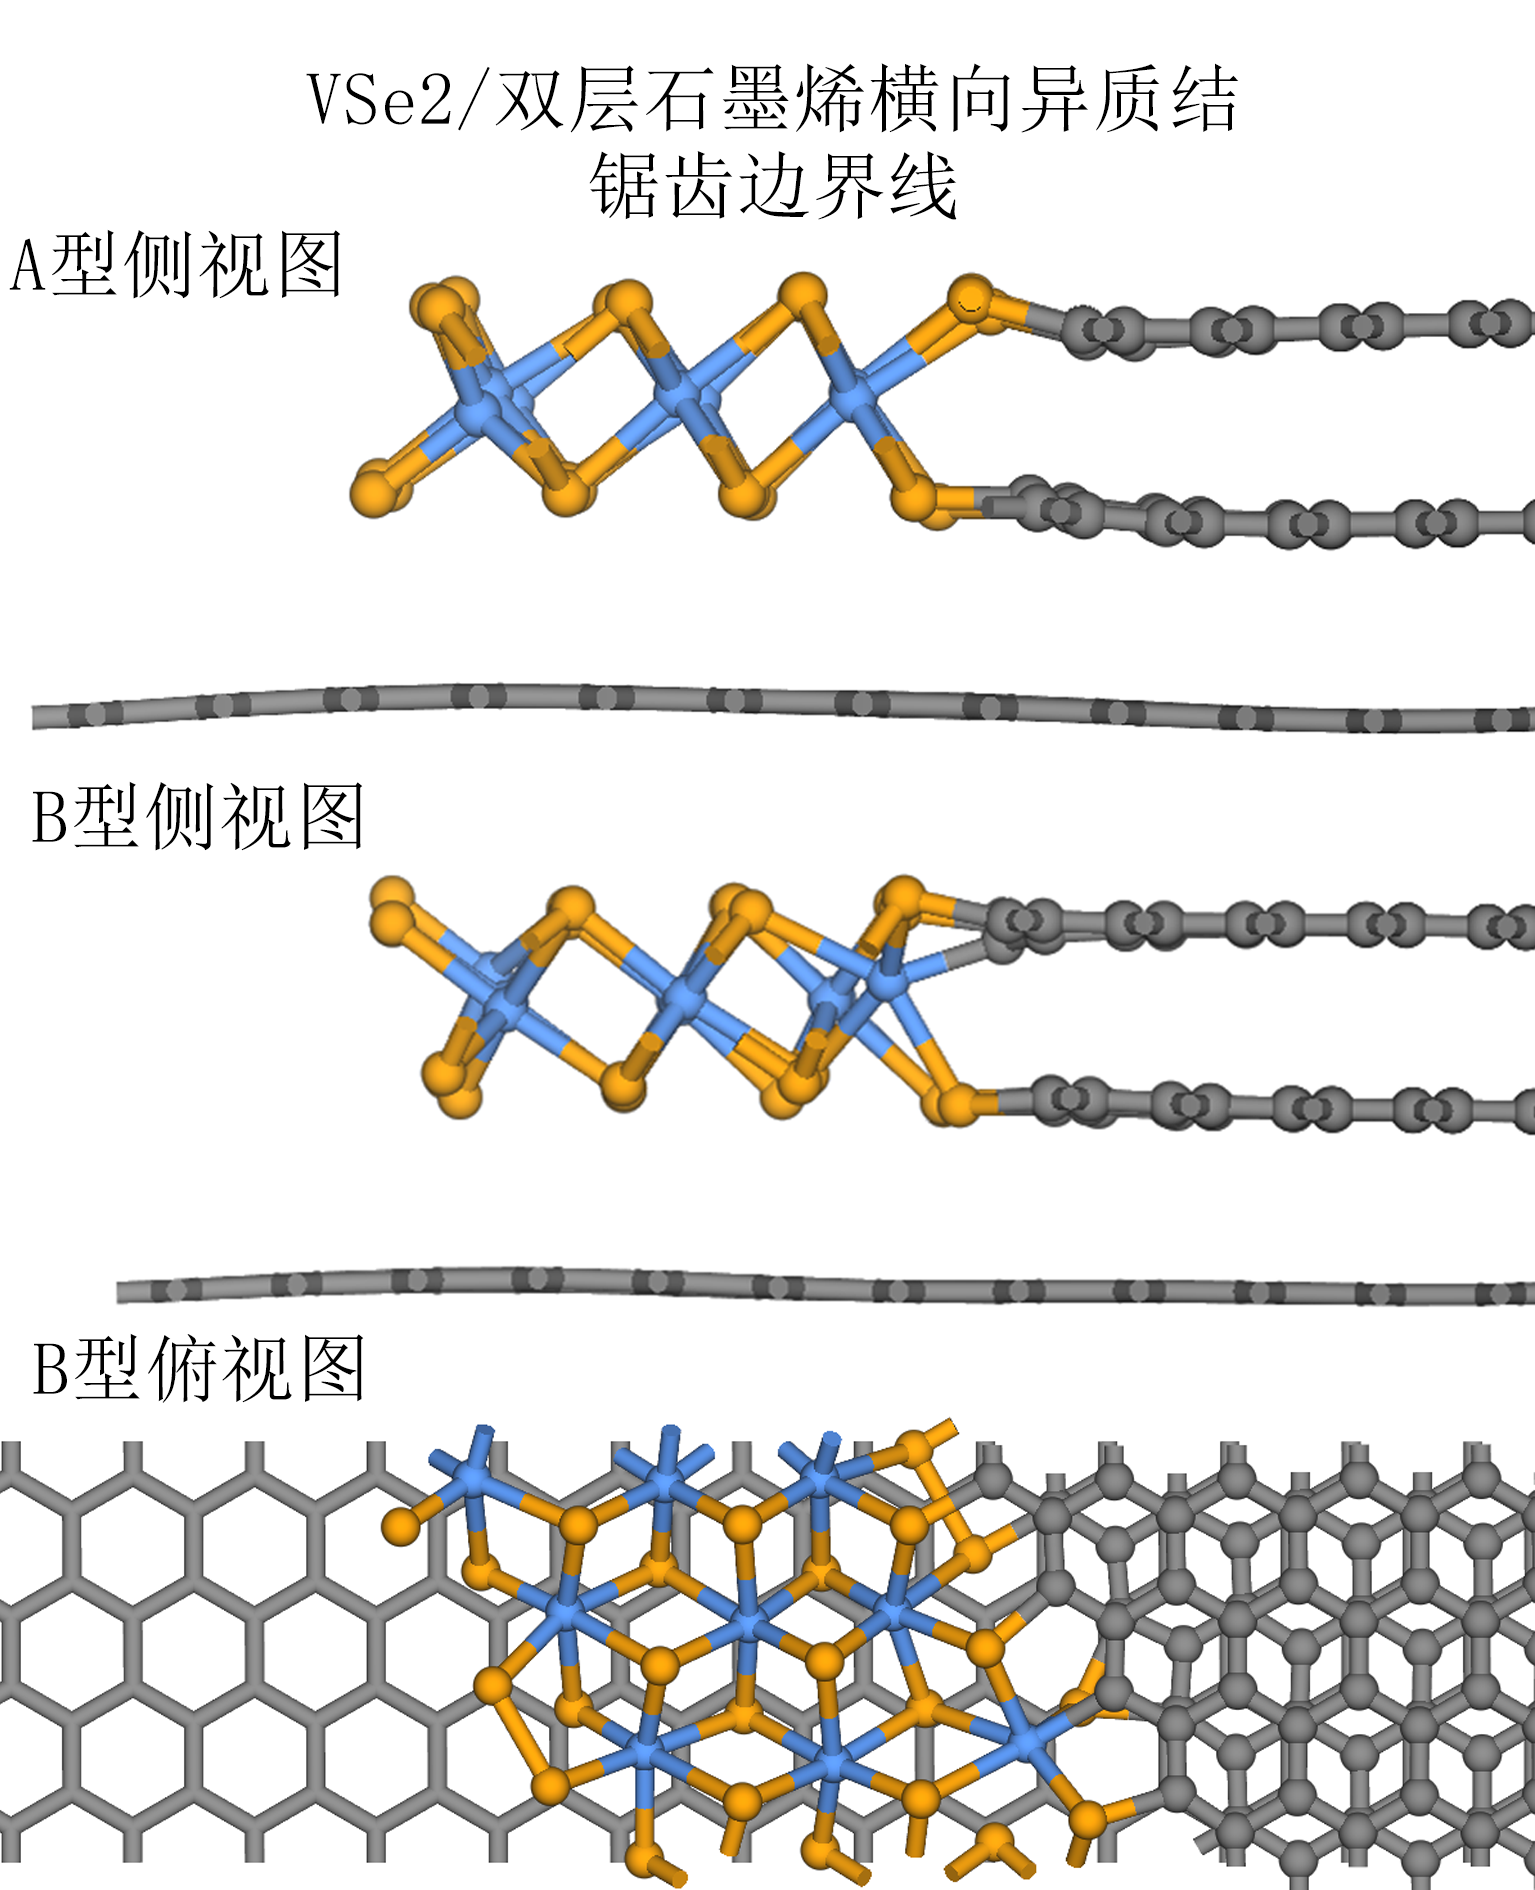
\includegraphics{pic/VS_structure_zigzag_VSe2-2SG.png}
            \label{fig:VS_structure_zigzag_VSe2-2SG}
        }
        \caption{石墨烯/\cemb{VSe2}三种横向二维异质结的原子结构图。(a)扶手椅边界线;(b)锯齿边界线。在原子结构图中,钒原子为蓝色;碳原子为灰色;硒原子为橙色。}
        \label{fig:VS_structure_ac_zz}
    \end{figure}

    由此,我们可以构建如图\ref{fig:VS_structure_ac_zz}三种不同的双层石墨烯/\cemb{VSe2}横向异质结的边界线匹配构型。对于扶手椅边界线,\cemb{VSe2}边缘的\cemb{V}原子与\cemb{Se}原子都与石墨烯边缘的\cemb{C}原子产生了一定的相互作用,双层石墨烯的高度正好对应于\cemb{VSe2}上下两个\cemb{Se}原子端面的高度。与\cemb{VSe}的扶手椅边缘成键后,原本位AB堆叠的双层石墨烯上下两层的堆叠方式产生了一定的偏移,

    而对于双层石墨烯与\cemb{VSe2}锯齿边缘之间的匹配,我们探究了两周不同的形式(图\ref{fig:VS_structure_zigzag_VSe2-2SG})。在A型锯齿边界中,\cemb{VSe2}与真空相接触的\cemb{Se}锯齿边缘相比于与底层石墨烯衬底接触的\cemb{Se}锯齿边缘更加侵入双层石墨烯台阶的内部。而在B型锯齿边界中,石墨烯/\cemb{VSe2}异质结在最底层的石墨烯表面进行了翻转,底层石墨烯衬底接触的\cemb{Se}锯齿边缘形成了嵌入双层石墨烯内部的边界线结构。

    为了探究石墨烯/\cemb{VSe2}横向异质结之间边界线的最优匹配模式,我们计算了各构型的界线的平均形成能密度$\varepsilon  $\chinesecolon
    \[
        \varepsilon = \frac{1}{l} \left( \energyVar{G/\ce{VSe2}}{} -\energyVar{G}{} -\energyVar{\ce{VSe2}}{} \right)
    \]
    其中,$\energyVar{G/\ce{VSe2}}{}$、$\energyVar{G}{}$和$\energyVar{\ce{VSe2}}{}$为石墨烯/\cemb{VSe2}横向异质结、组成横向异质结的单独状态下的石墨烯和单独状态下的\cemb{VSe2}的计算总能量。$l$为石墨烯/\cemb{VSe2}横向异质结的边界线的长度。
    
    \begin{figure}[htb]
        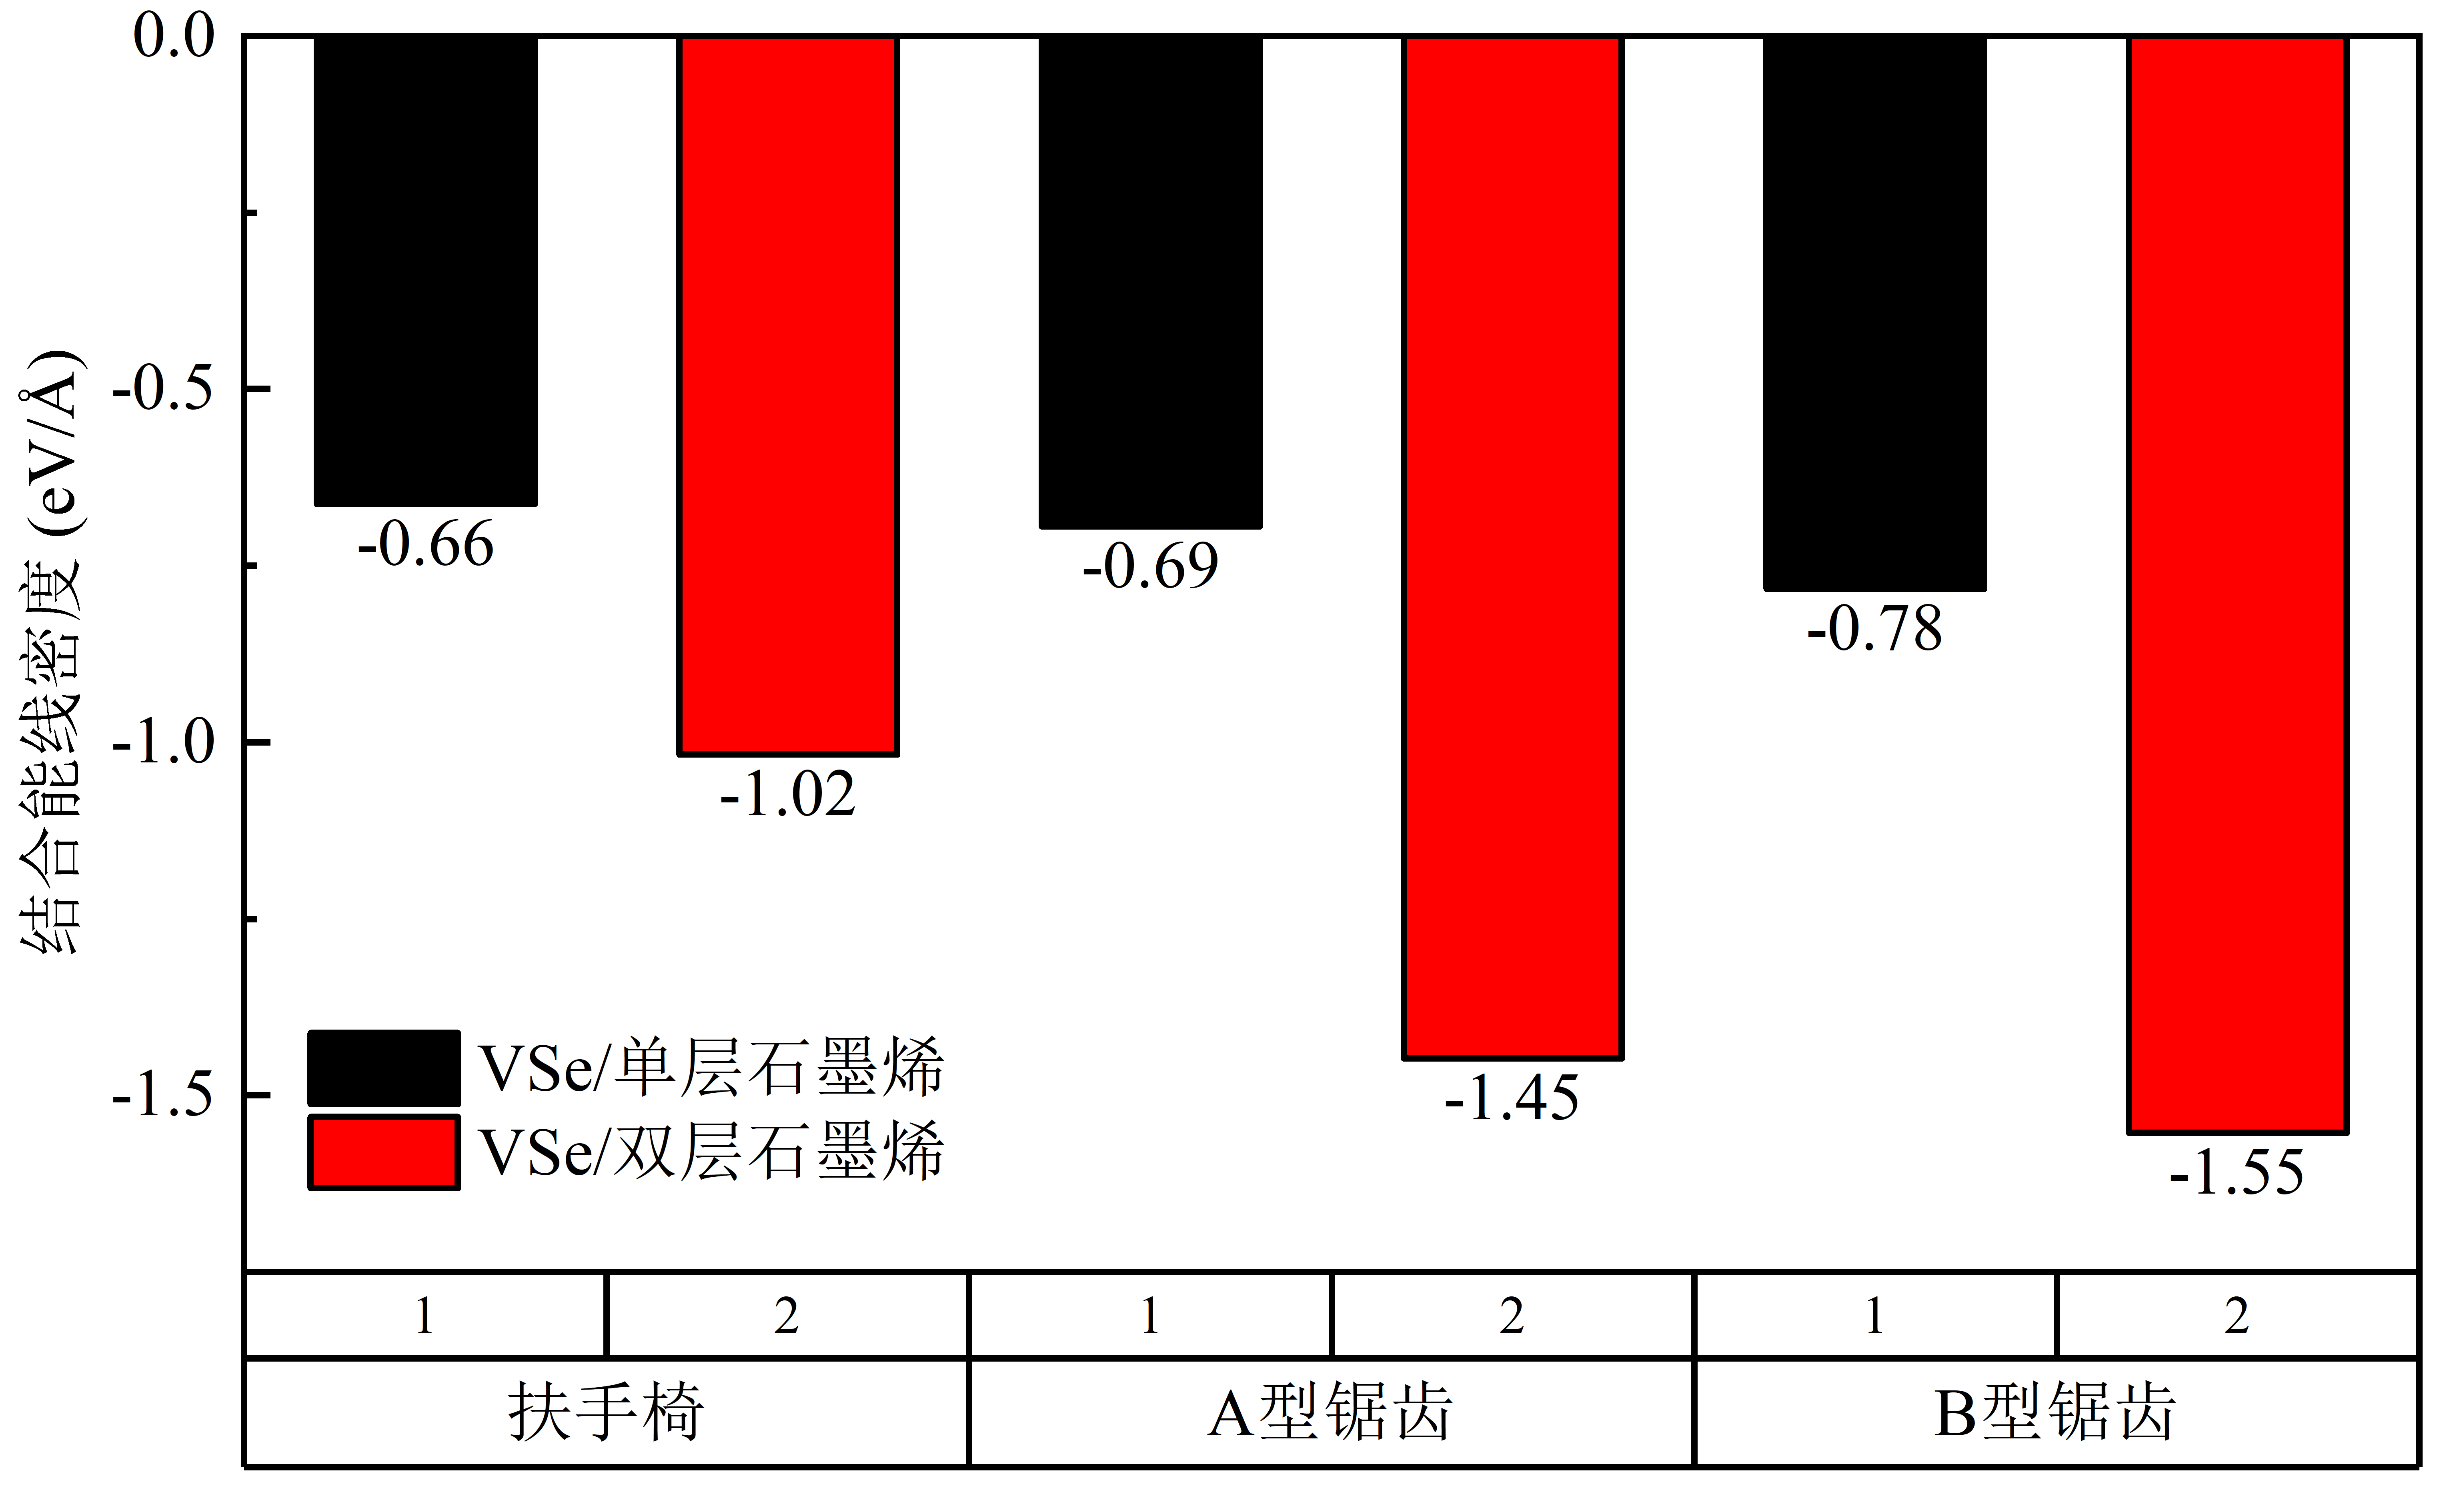
\includegraphics{pic/VS_DFT_VSe2-G_stepAndEdge.png}
        \caption{不同构型的石墨烯/\cemb{VSe2}横向异质结的平均边界结合能密度。}
        \label{fig:VS_DFT_VSe2-G_stepAndEdge}
    \end{figure}

    在图\ref{fig:VS_DFT_VSe2-G_stepAndEdge}中,我们计算了单层、双层石墨烯和\cemb{VSe2}组成的横向异质结的平均边界结合能密度。
    对于单层石墨烯台阶与\cemb{VSe2}组成的横向异质结,边界结合最弱的形态为扶手椅匹配,此时的平均结合能密度为\SI{-0.66}{\electronvolt\per\angstrom}。形成A型锯齿匹配的单层石墨烯/\cemb{VSe2}横向异质结的结合边界稍稍强与扶手椅匹配,平均结合能密度达到了\SI{-0.78}{\electronvolt\per\angstrom}。而形成B型锯齿匹配的单层石墨烯/\cemb{VSe2}横向异质结在三种边界匹配中具有最高的结合强度,达到了\SI{-0.78}{\electronvolt\per\angstrom}。

    对于在双层的石墨烯台阶的边缘形成的\cemb{VSe2}横向二维异质结,石墨烯/\cemb{VSe2}边界线处的平均结合能均高于在单层的石墨烯台阶的结合能。和单层石墨烯台阶时类似,\cemb{VSe2}与双层石墨烯台阶匹配时相比于形成扶手椅型匹配的边界线更倾向于形成锯齿形匹配。当形成扶手椅匹配的时,\cemb{VSe2}与双层石墨烯台阶边界线的形成能密度为\SI{-1.02}{\electronvolt\per\angstrom}。将扶手椅匹配变为锯齿匹配则可以将边界线的形成能密度大幅下降。B型锯齿匹配为双层石墨烯和单层\cemb{VSe2}横向异质结边界线的最优匹配构型,其平均结合能密度为\SI{-1.55}{\electronvolt\per\angstrom},略高于A型锯齿匹配的\SI{-1.45}{\electronvolt\per\angstrom}。

    石墨烯/\cemb{VSe2}中A、B型锯齿匹配的边界结合强度的差异主要来自最下层石墨烯衬底对于边界处\cemb{C}原子和\cemb{Se}原子之间相互作用的耦合。如图\ref{fig:VS_structure_zigzag_VSe2-2SG}所示,在石墨烯与\cemb{VSe2}相接触的位置,B型锯齿边界处最下方的石墨烯衬底呈现出略微下凹的结构,而A型锯齿边界处的衬底则为褶皱起伏状。

    综合上述的计算结果,我们可以推断从热力学的角度,单层的\cemb{VSe2}可以自发地在单层或者双层石墨烯台阶的边缘生长,形成石墨烯
    /\cemb{VSe2}横向异质结。同时我们的计算显示对于1T相的\cemb{VSe2},石墨烯台阶的锯齿形边缘相比于扶手椅型的边缘更容易形成石墨烯/\cemb{VSe2}横向异质结。

    由于在具有台阶的少层石墨烯上生长\cemb{VSe2}时,作为生长物质源的\cemb{V}原子和\cemb{Se}原子大多先沉积到石墨烯的表面,再通过表面迁移的方式参与到\cemb{VSe2}的生长之中。接下来,我们通过研究\cemb{V}原子和\cemb{Se}原子在单层和双层石墨烯/\cemb{VSe2}横向异质结的边界线处的扩散行为,来对\cemb{VSe2}在单、双层石墨烯台阶边缘进行生长时的动力学行为进行解构。

    \begin{figure}[htb]
        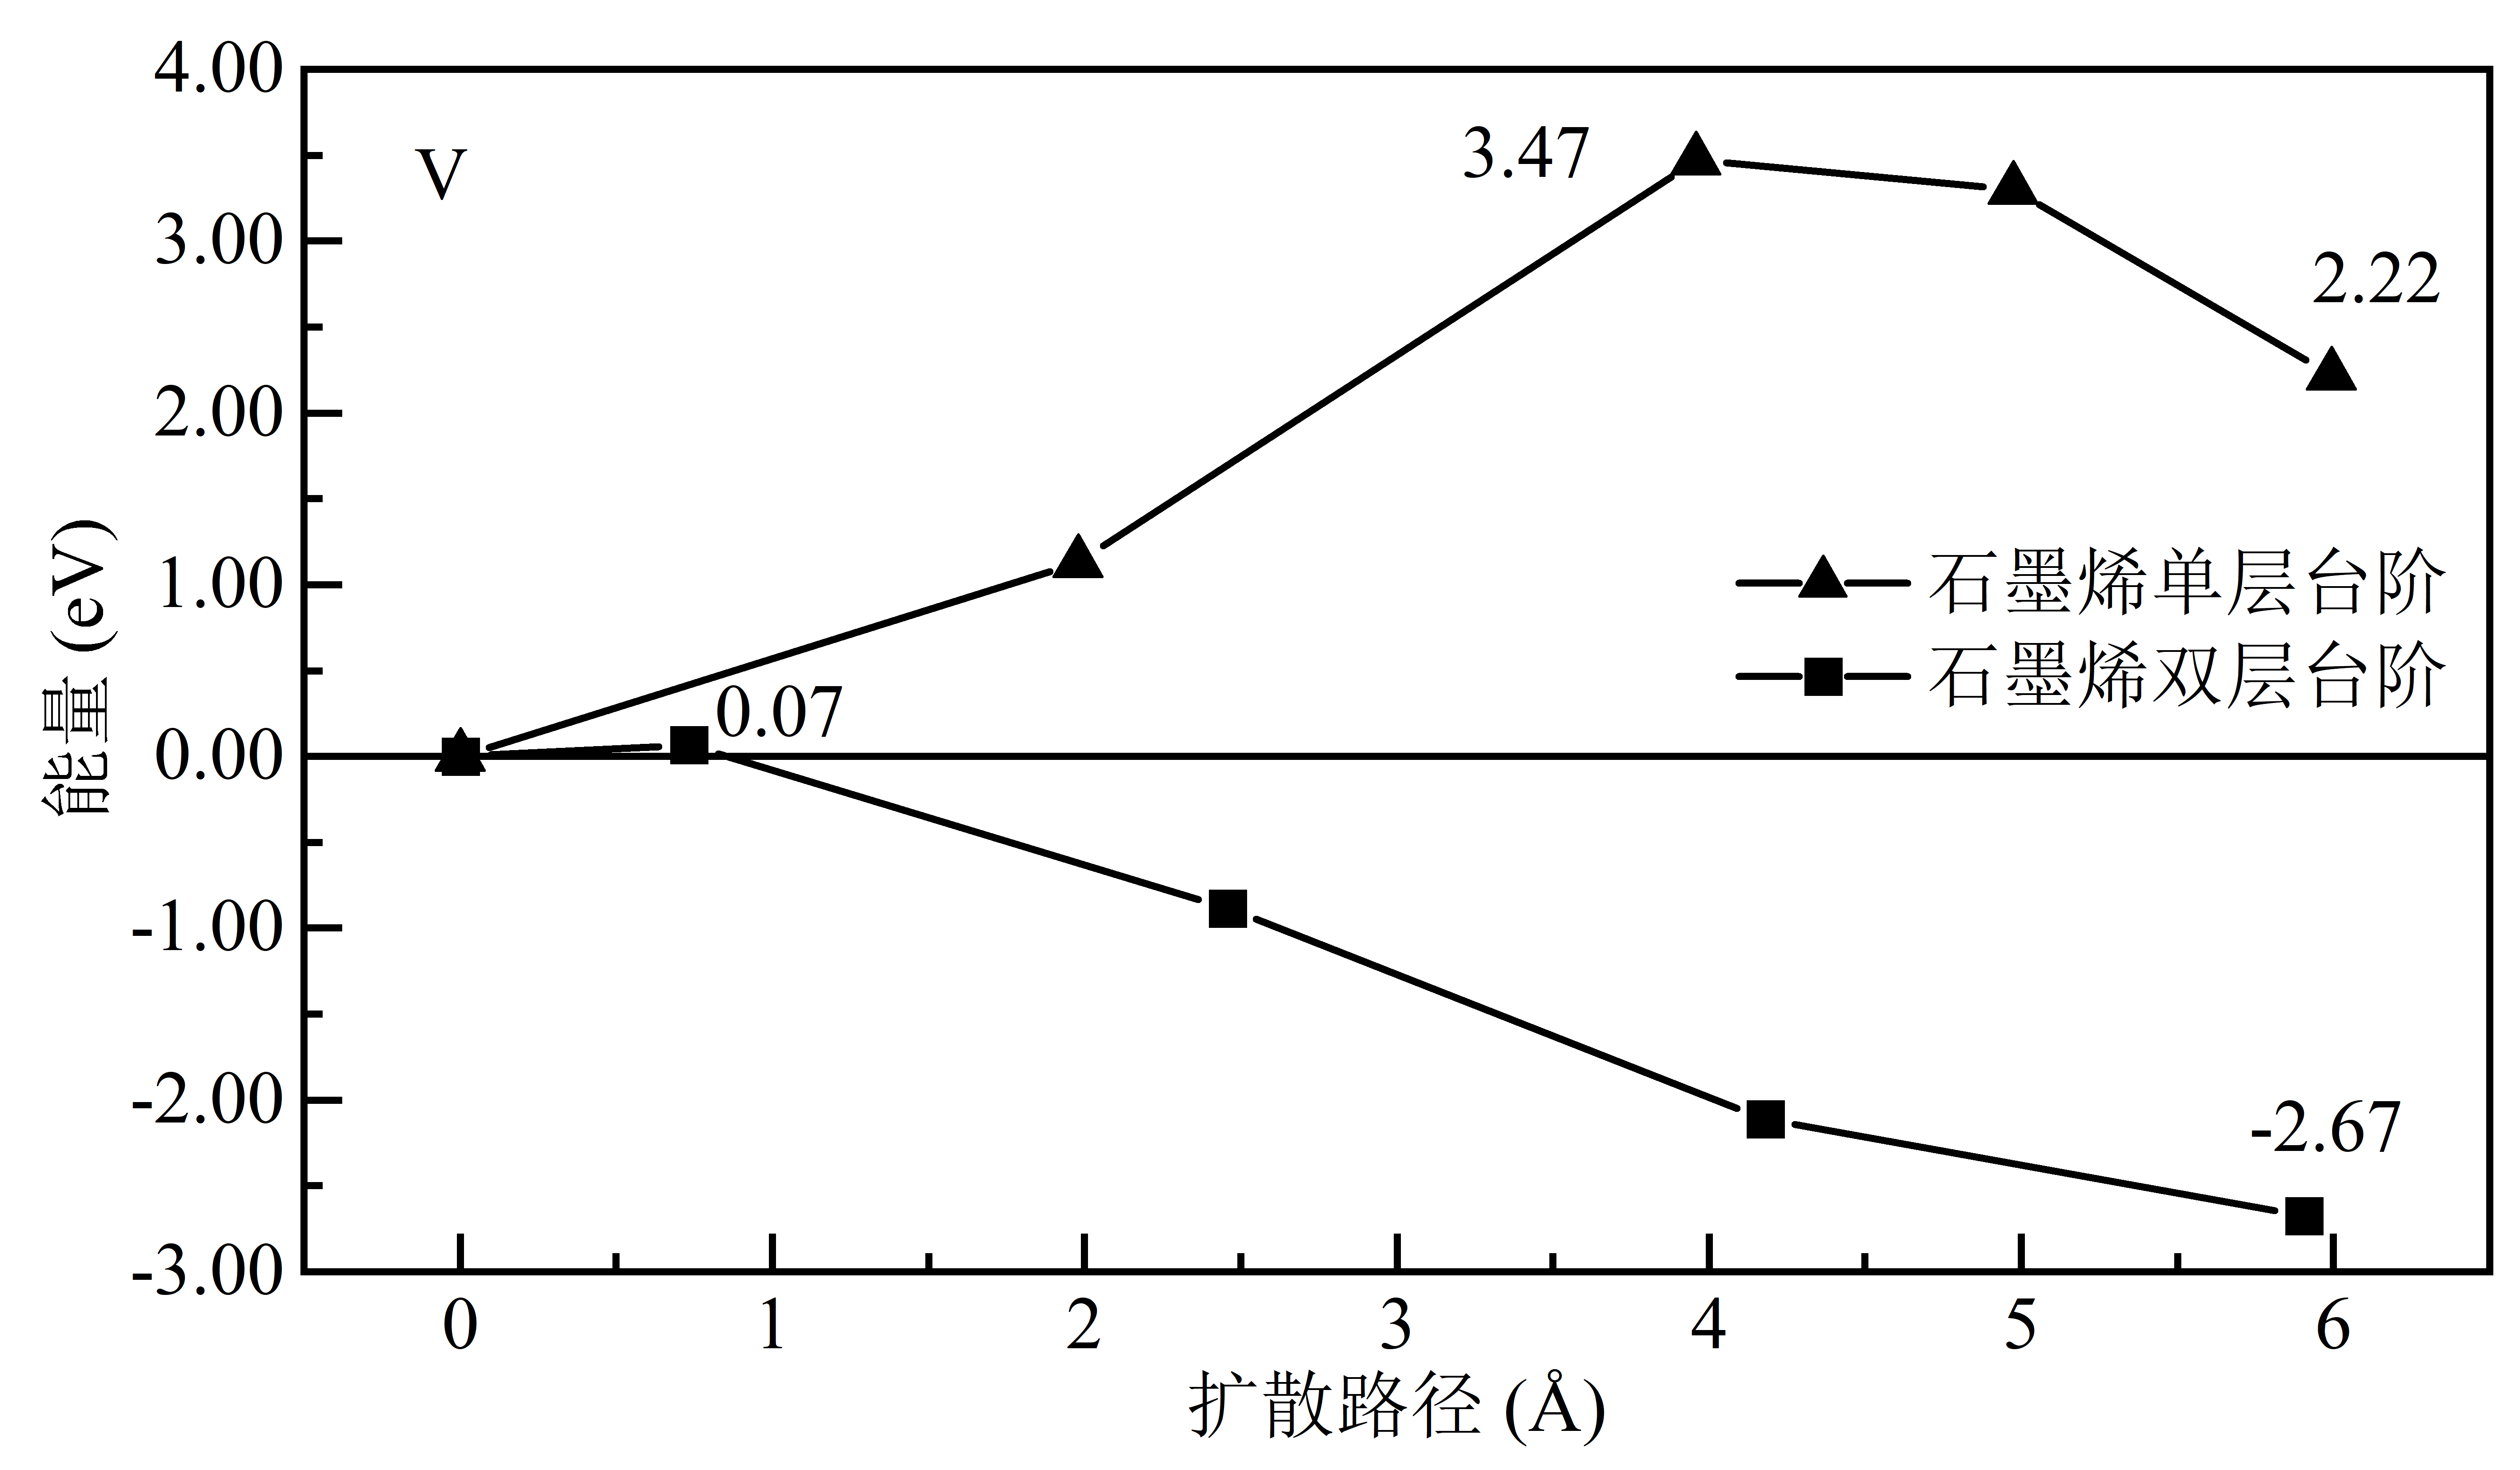
\includegraphics{pic/VS_DFT_NEB_V_GtVSe.png}
        \caption{\cemb{V}原子在单、双层石墨烯/\cemb{VSe2}横向异质结边界线处的扩散能量曲线。}
        \label{fig:VS_DFT_NEB_V_GtVSe}
    \end{figure}

    在图\ref{fig:VS_DFT_NEB_V_GtVSe}中,我们计算并且绘制了\cemb{V}原子在单双层石墨烯/\cemb{VSe2}横向异质结边界线处的扩散能量曲线。可以看到,对于单层石墨烯/\cemb{VSe2}横向异质结的边界线,\cemb{V}原子需要跨越高达\SI{3.47}{\electronvolt}的势垒才能够从单层石墨烯台阶的表面扩散至\cemb{VSe2}的表面,参与后续\cemb{VSe2}的生长。同时,在单层石墨烯/\cemb{VSe2}异质结中,\cemb{V}原子在边界线石墨烯侧的能量比在边界线\cemb{VSe2}侧的能量低\SI{2.22}{\electronvolt}。这表示\cemb{V}原子在单层石墨烯到\cemb{VSe2}的扩散过程不仅需要跨越极高的扩散势垒,还需要吸较高的能量。导致在热平衡状态下,停留在单层石墨烯台阶表面的\cemb{V}原子的比例要远高于停留在相接的\cemb{VSe2}表面的\cemb{V}原子的比例。
    
    \begin{figure}[htb]
        \subfloat[]{
            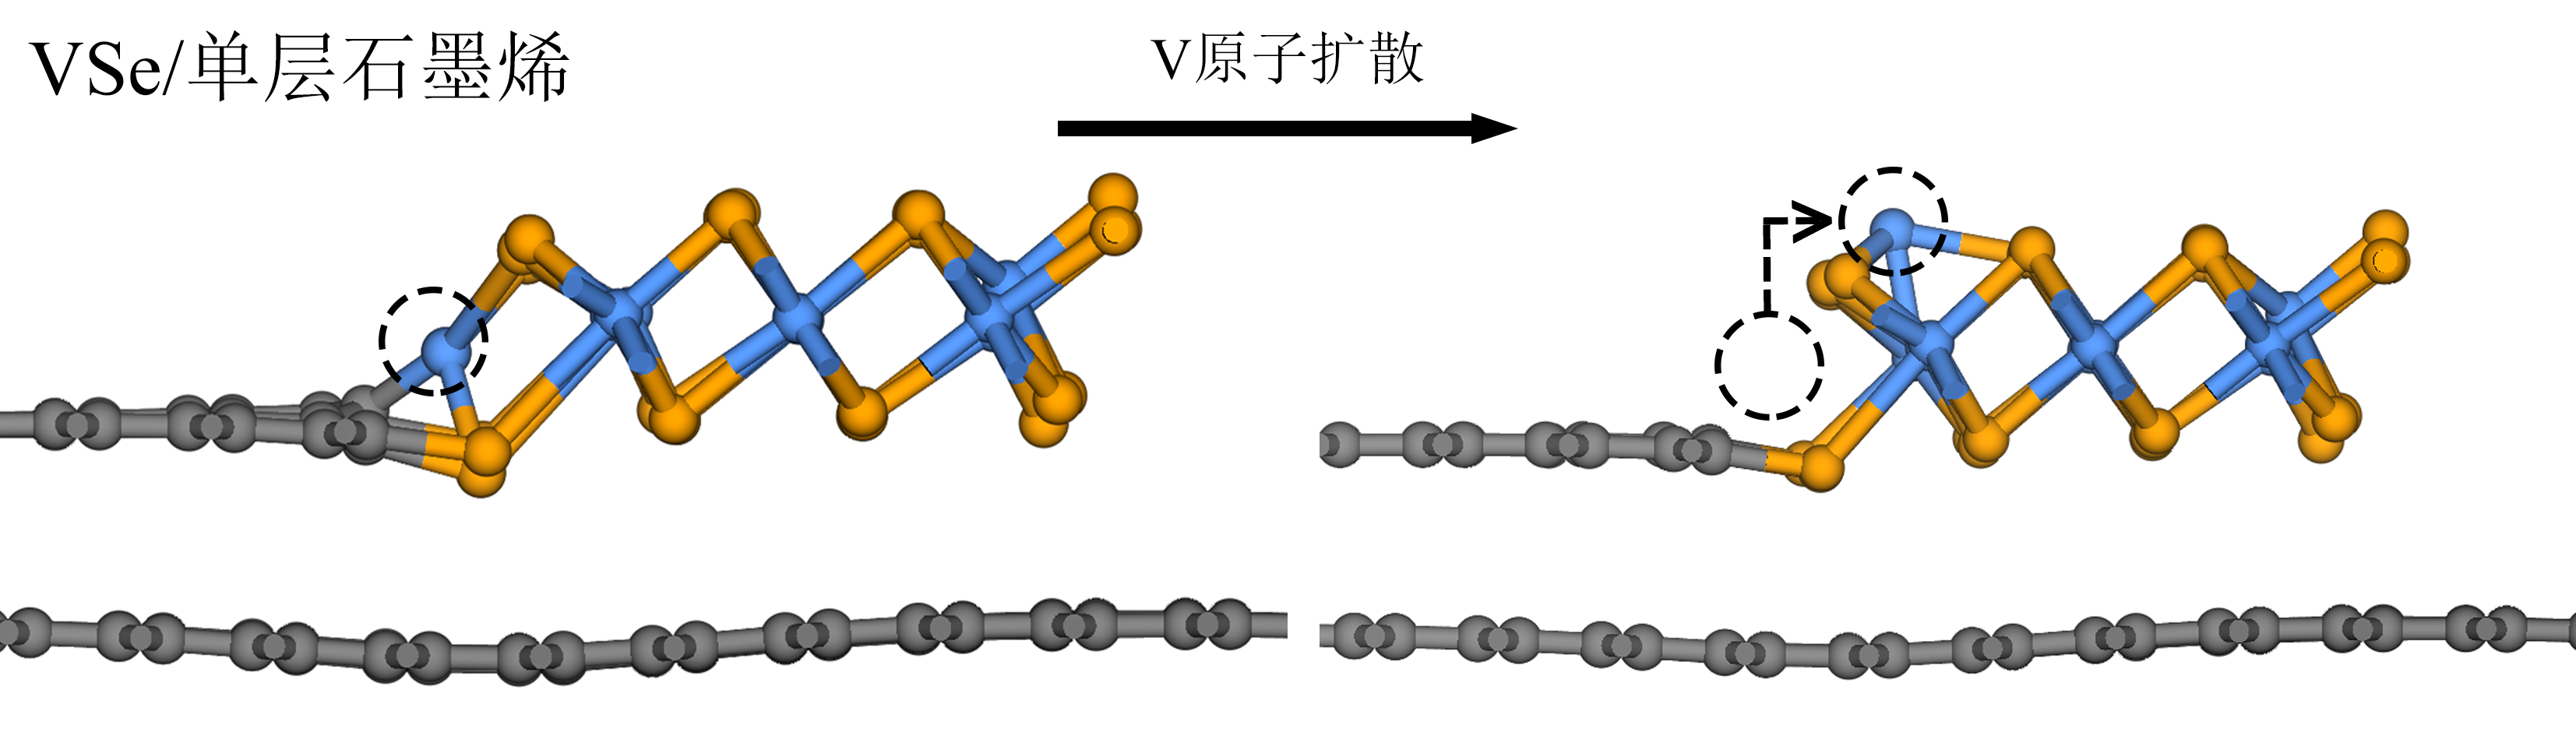
\includegraphics{pic/VS_structure_VNeb1SG.png}
            \label{fig:VS_structure_VNeb1SG}
        }\\[-0.5ex]
        \subfloat[]{
            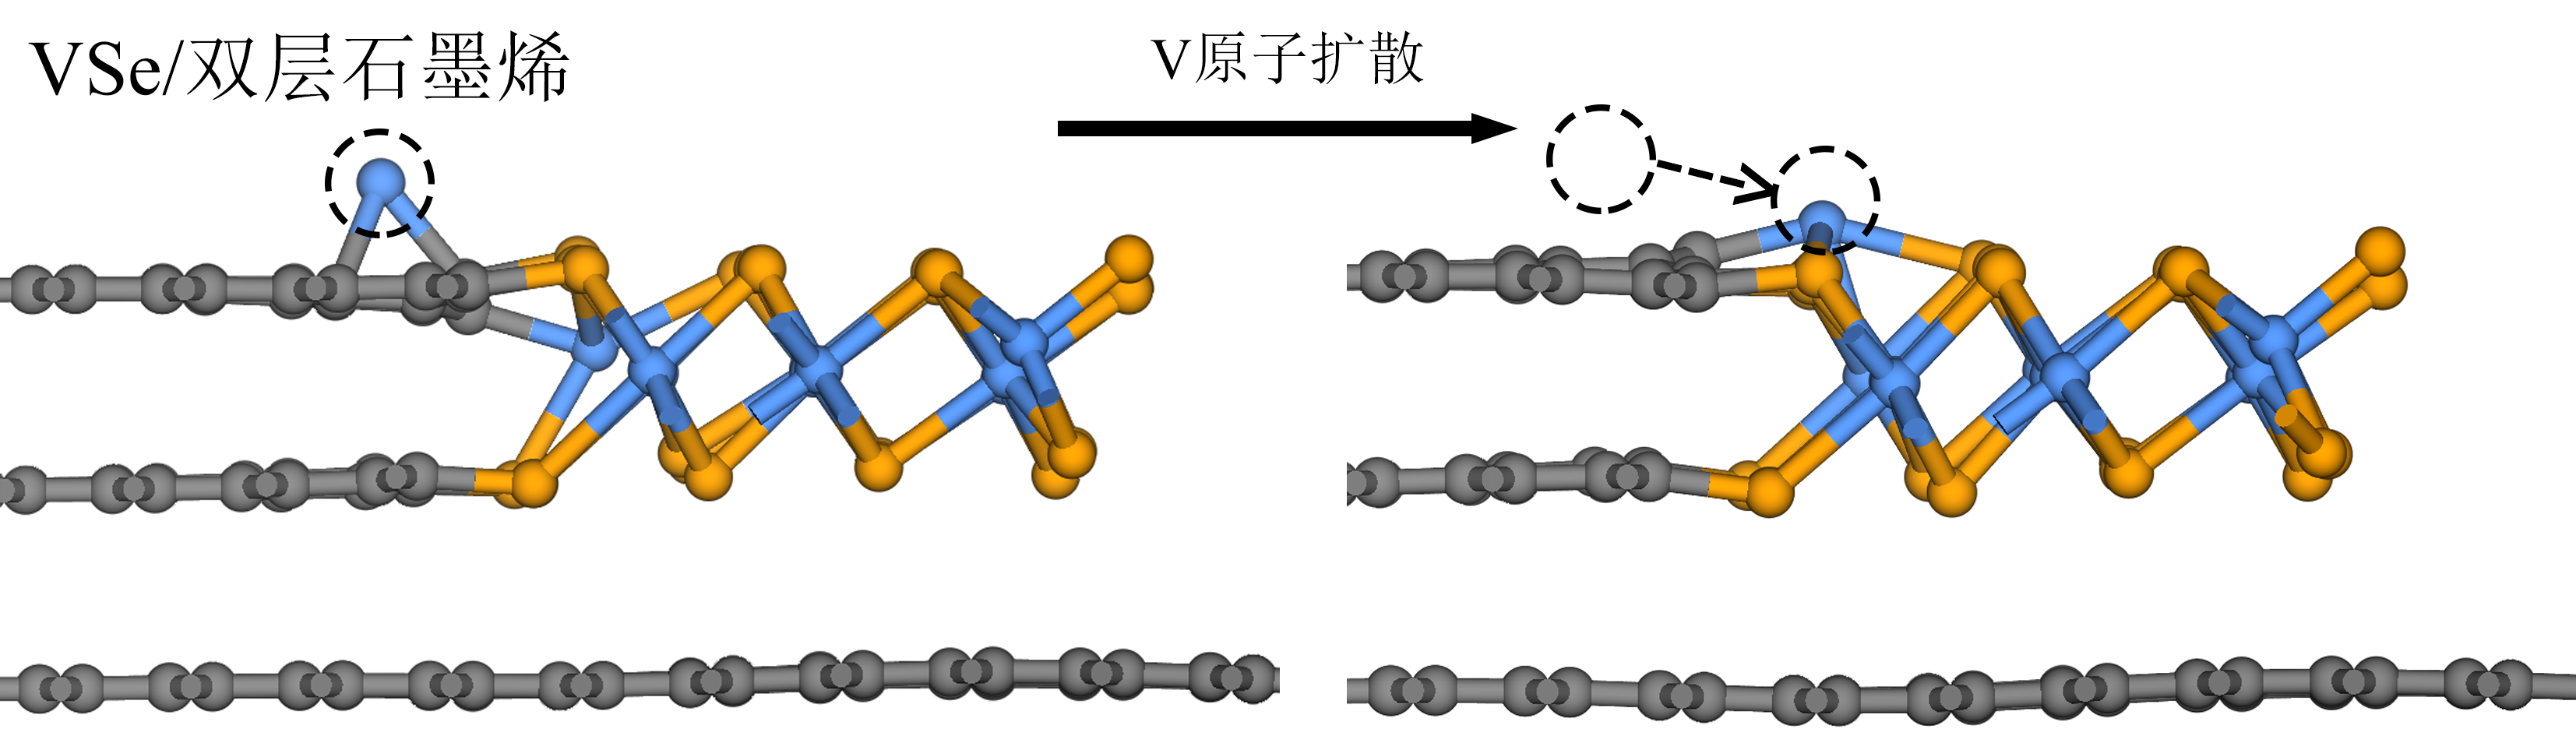
\includegraphics{pic/VS_structure_VNeb2SG.png}
            \label{fig:VS_structure_VNeb2SG}
        }
        \caption{\cemb{V}原子在单、双层石墨烯与\cemb{VSe2}形成的横向异质结的边界线处的扩散路径和原子结构示意图。(a)单层石墨烯/\cemb{VSe2}横向异质结边界线处的扩散;(b)双层石墨烯/\cemb{VSe2}横向异质结边界线处的扩散。在原子结构图中,钒原子为蓝色;碳原子为灰色;硒原子为橙色。}
        \label{fig:VS_structure_VNeb}
    \end{figure}

    从\cemb{V}原子在单层石墨烯/\cemb{VSe2}的边界线处迁移前后的原子结构(图\ref{fig:VS_structure_VNeb1SG})我们也可以看到。在单层石墨烯一侧吸附的\cemb{V}原子需要脱离于石墨烯边缘\cemb{C}原子和\cemb{VSe2}层下方\cemb{Se}原子的相互作用,向上穿过\cemb{VSe2}层上方的\cemb{Se}原子之间的空隙,到达边界线\cemb{VSe2}侧的\cemb{V}原子上方,与上方的\cemb{Se}原子成键。

    动力学和热力学上如此困难的扩散路径会导致与单层石墨烯台阶相连的\cemb{VSe2}表面缺少游离的\cemb{V}原子,进而阻碍\cemb{VSe2}的后续生长。

    而对于双层石墨烯/\cemb{VSe2},\cemb{V}原子在边界线处的扩散能量曲线更为平坦。从双层石墨烯的表面迁移至相接的\cemb{VSe2}的表面,\cemb{VSe2}只需要跨越\SI{0.07}{\electronvolt}的势垒。同时,在\cemb{VSe2}侧的表面,\cemb{V}原子的能量比在双层石墨烯一侧的表面要低\SI{-2.67}{\electronvolt}。更低的能量使得\cemb{V}原子能够由双层石墨烯的一侧的表面自发的扩散至\cemb{VSe2}一侧的表面。

    从\cemb{V}原子在双层石墨烯/\cemb{VSe2}边界处的扩散路径(图\ref{fig:VS_structure_VNeb})也可以看出,由于双层石墨烯和单层\cemb{VSe2}相似的原子层厚度,\cemb{V}原子从石墨烯一侧扩散至\cemb{VSe2}一侧的过程中不需要进行原子层台阶的攀爬,导致了较小的扩散势垒。同时,由于第二层石墨烯台阶边缘的\cemb{C}原子在一定程度上饱和了\cemb{VSe2}上方的\cemb{Se}原子,使得\cemb{V}原子在石墨烯一侧仅与石墨烯表面的\cemb{C}原子成键。而当\cemb{V}原子扩散至边界线的\cemb{VSe2}一侧时,\cemb{V}原子和\cemb{VSe2}表面强烈的相互作用使得\cemb{V}原子部分嵌入\cemb{VSe2}上表面的\cemb{Se}原子层中,导致了\cemb{V}原子在\cemb{VSe2}一侧的能量远低于在双层石墨烯一侧的能量。

    动力学上较低的扩散势垒和热力学上较高的能量驱动力使得\cemb{V}原子很容易从双层石墨烯的表面扩散至相接的\cemb{VSe2}的表面。使得\cemb{VSe2}表面具有较为充足的游离\cemb{V}原子供\cemb{VSe2}进行生长。

    \begin{figure}[htb]
        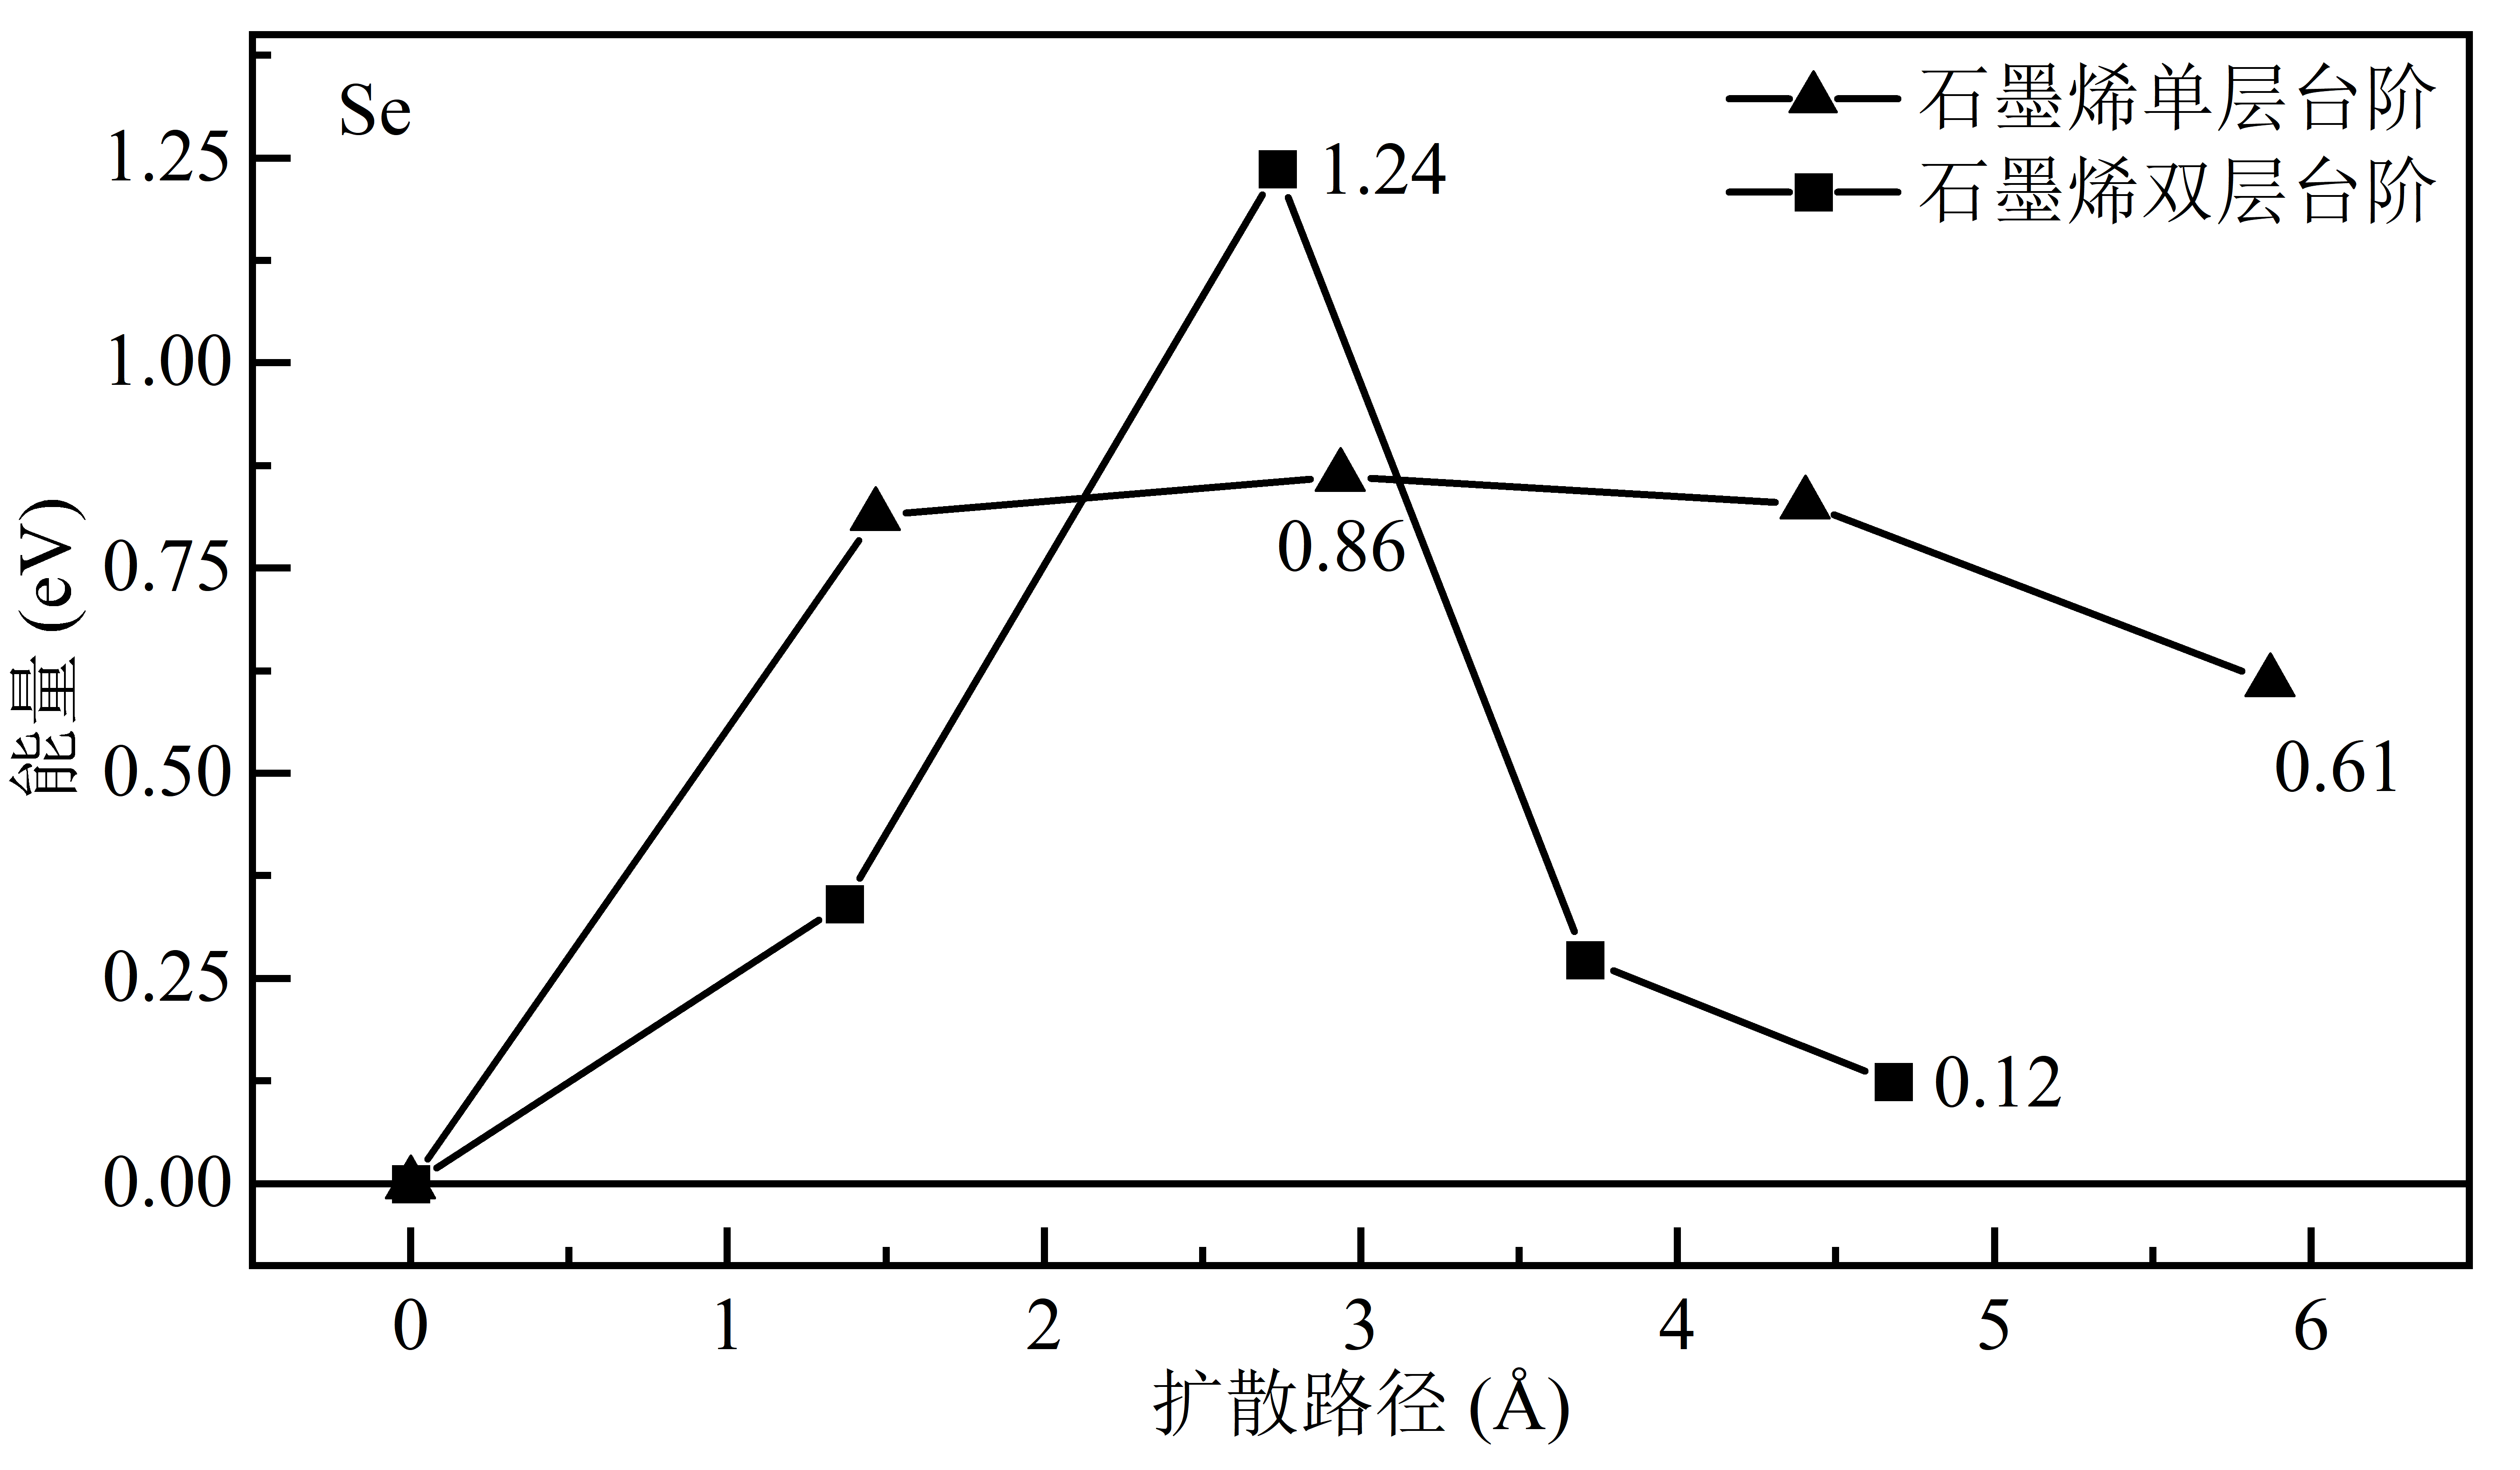
\includegraphics{pic/VS_DFT_NEB_Se_GtVSe.png}
        \caption{\cemb{Se}原子在单、双层石墨烯/\cemb{VSe2}横向异质结边界线处的扩散能量曲线。}
        \label{fig:VS_DFT_NEB_Se_GtVSe}
    \end{figure}

    对于\cemb{Se}原子在单、双层石墨烯/\cemb{VSe2}横向异质结边界线处的扩散行为,我们在图\ref{fig:VS_DFT_NEB_Se_GtVSe}中绘制了相应的能量曲线。对于单层石墨烯\cemb{VSe2}横向异质结,\cemb{Se}原子从边界线的单层石墨烯一侧扩散至\cemb{VSe2}一侧需要跨越\SI{0.86}{\electronvolt}的扩散势垒。从始末状态看,\cemb{Se}原子从石墨烯一侧迁移至\cemb{VSe2}一侧需要吸收\SI{0.61}{\electronvolt}的能量。对于\cemb{Se}原子,在单层石墨烯/\cemb{VSe2}异质结边界线上扩散的势垒和反应能均小于\cemb{V}原子扩散的情况。在热平衡下,大多数的\cemb{Se}原子停留在单层石墨烯以及石墨烯一侧的边界线处,有部分\cemb{Se}原子在热动能的作用下吸收能量跨越迁移势垒进入\cemb{VSe2}一侧,参与后续\cemb{VSe2}的生长。
    
    \cemb{Se}原子在双层石墨烯/cemb{VSe2}边界线处的扩散行为与\cemb{V}原子扩散有较大普通。从边界线的双层石墨烯一侧扩散至\cemb{VSe2}一侧,\cemb{Se}原子需要跨越\SI{1.24}{\electronvolt}的能量势垒。这个能量势垒高于\cemb{Se}原子跨越单层石墨烯/\cemb{VSe2}边界线的势垒高度。但边界线的在\cemb{VSe}一侧,\cemb{Se}原子的能量相比于在双层石墨烯的一侧仅高了\SI{0.12}{\electronvolt}。更低的扩散反应能量意味着在双层石墨烯/\cemb{VSe2}异质结上,\cemb{Se}原子扩散至边界线的\cemb{VSe2}一侧的比例高于在单层石墨烯/\cemb{VSe2}上的情况。与\cemb{V}原子在单、双层石墨烯/\cemb{VSe2}边界处扩散行为不同的是,\cemb{Se}原子在平坦的双层石墨烯/\cemb{VSe2}边界线处扩散的扩散势垒(\SI{1.24}{\electronvolt})高于需要翻越半个原子台阶的单层石墨烯/\cemb{VSe2}边界处的扩散。
    
    \begin{figure}
        \subfloat[]{
            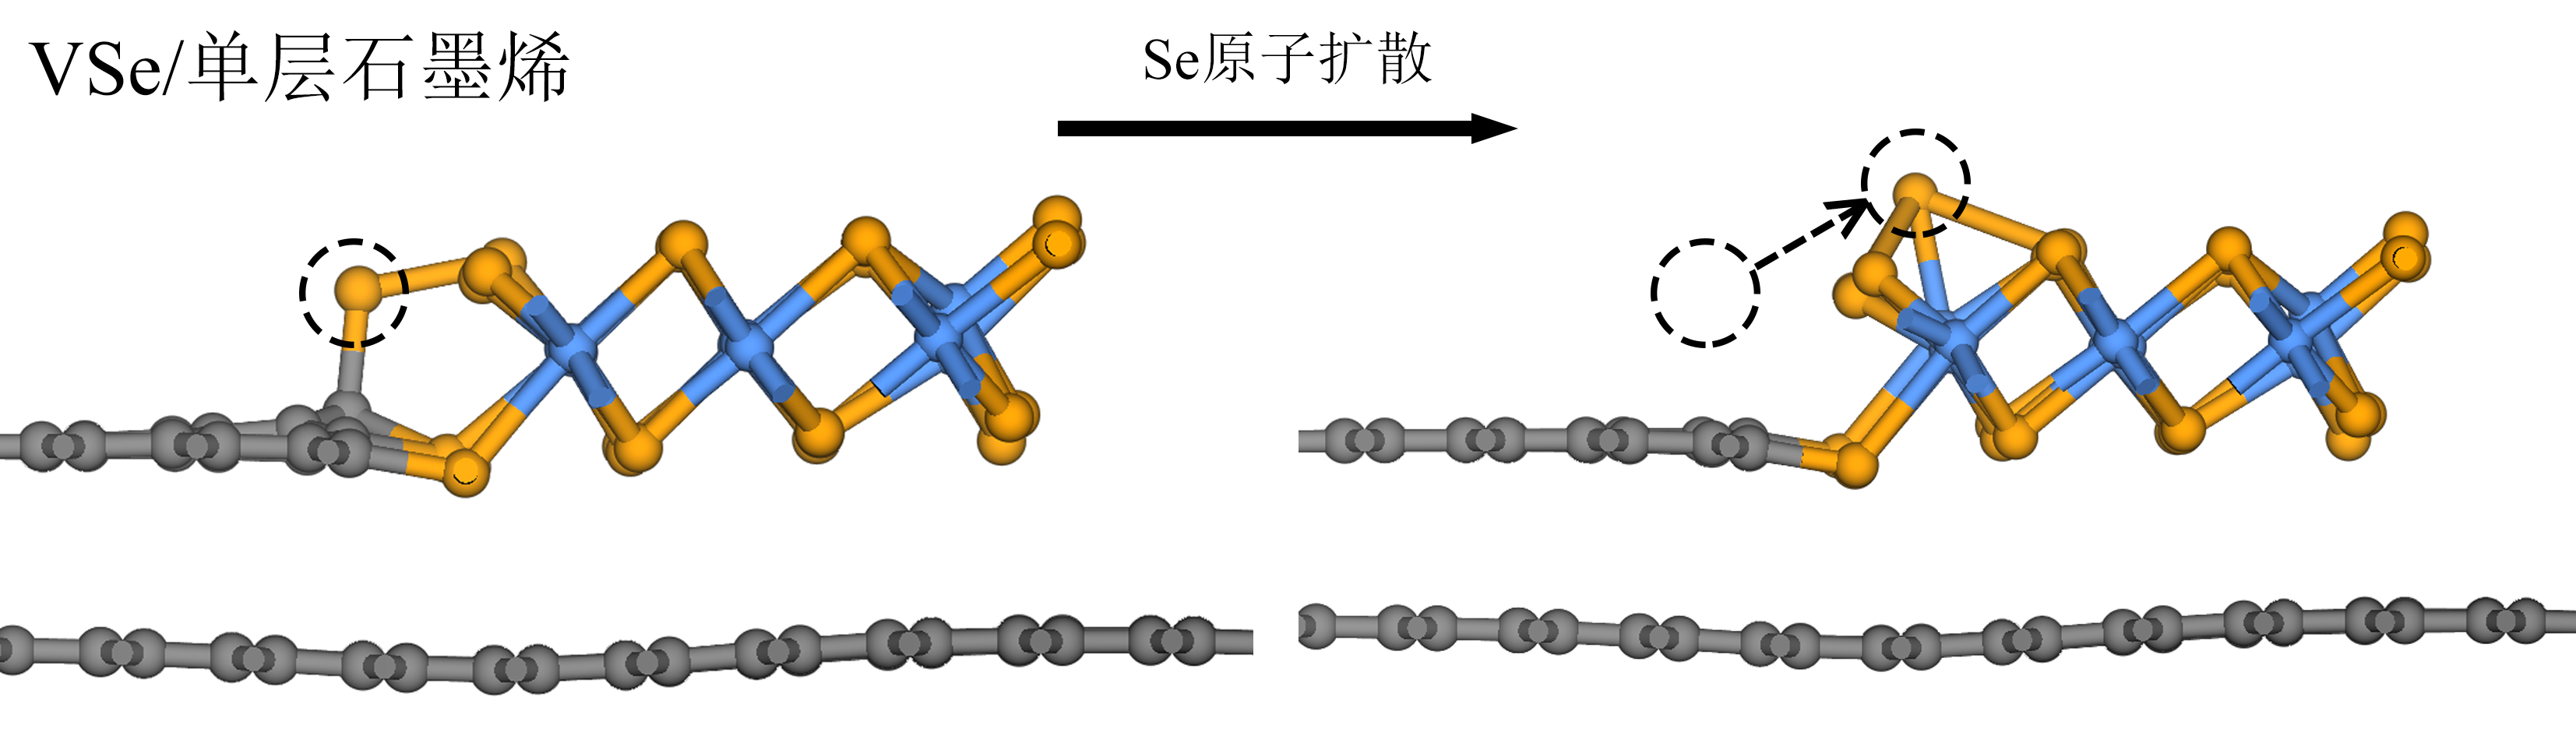
\includegraphics{pic/VS_structure_SeNeb1SG.png}
            \label{fig:VS_structure_SeNeb1SG}
        }\\[-0.5ex]
        \subfloat[]{
            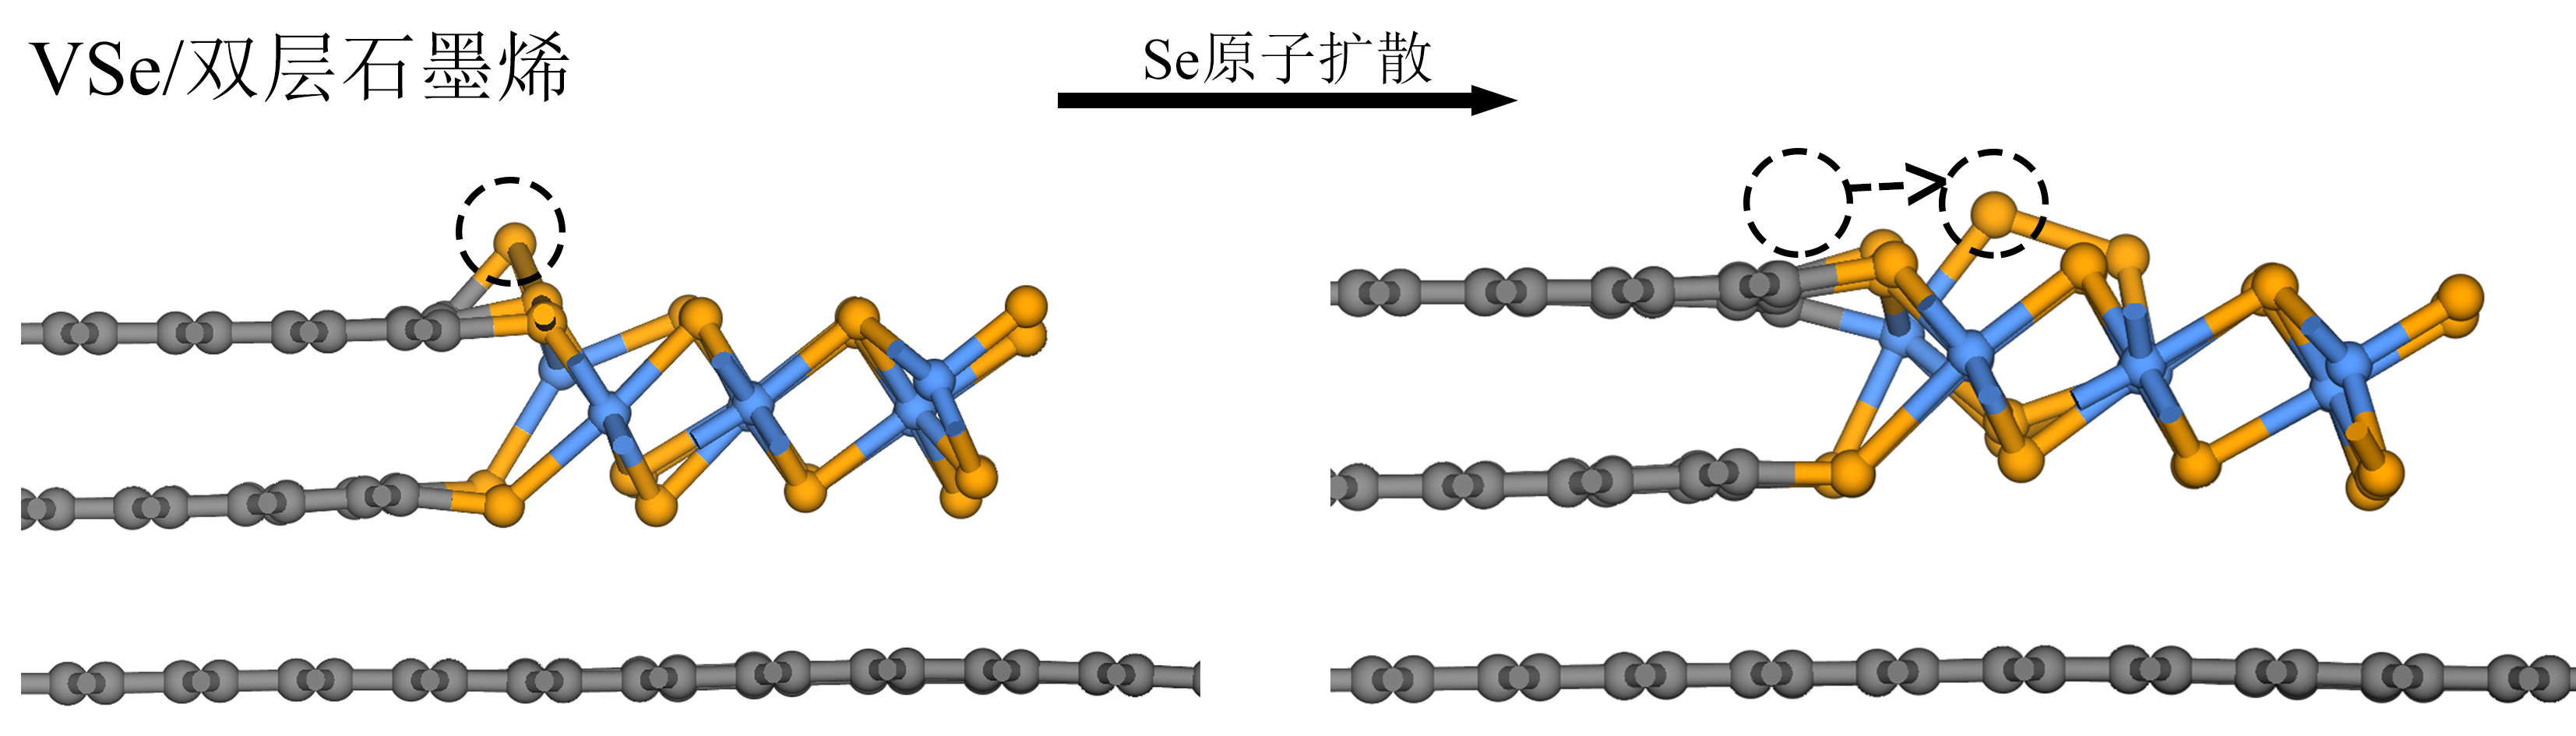
\includegraphics{pic/VS_structure_SeNeb2SG.png}
            \label{fig:VS_structure_SeNeb2SG}
        }
        \caption{\cemb{Se}原子在单、双层石墨烯与\cemb{VSe2}形成的横向异质结的边界线处的扩散路径和原子结构示意图。(a)单层石墨烯/\cemb{VSe2}横向异质结边界线处的扩散;(b)双层石墨烯/\cemb{VSe2}横向异质结边界线处的扩散。在原子结构图中,钒原子为蓝色;碳原子为灰色;硒原子为橙色。}
        \label{}
    \end{figure}

    从扩散前后的原子结构来看,在单层石墨烯/\cemb{VSe2}横向异质结边界处的石墨烯一侧,游离的\cemb{Se}原子与\cemb{VSe2}的上表面\cemb{Se}成键。相比于与下表面\cemb{Se}成键的\cemb{V}原子,\cemb{Se}原子在单层石墨烯上成键时的高度与相接\cemb{VSe2}的上表面更加接近。同时,在扩散过程中,\cemb{Se}原子只需要断裂与单层石墨烯表面\cemb{C}原子之间的相互作用,使得\cemb{Se}原子在单层石墨烯/\cemb{VSe2}边界线扩散时的扩散势垒远低与\cemb{V}原子扩散的情况。而对于游离的\cemb{Se}原子在双层石墨烯/\cemb{VSe2}的边界线处的扩散行为。在双层石墨烯一侧,\cemb{Se}原子同时与第二层石墨烯边界的\cemb{C}原子以及\cemb{VSe2}边界的上表面\cemb{Se}原子产生了较强的相互作用。在扩散至边界线的\cemb{VSe2}一侧的过程中,游离的\cemb{Se}原子需要断开与边界线处\cemb{Se}原子的成键,由此导致了\cemb{Se}在双层石墨烯/\cemb{VSe2}表面较高的扩散势垒。

    对比\cemb{V}原子在单、双石墨烯/\cemb{VSe2}边界线处的扩散行为,在双层石墨烯/\cemb{VSe2}表面扩散的游离\cemb{V}原子能够自发的从双层石墨烯的一侧向\cemb{VSe2}的一侧扩散。而对于游离的\cemb{Se}原子,无论是在具有高度差的单层石墨烯/\cemb{VSe2}横向异质结还是在平坦的双层石墨烯\cemb{VSe2}横向异质结,都需要吸收一定的能量才能够从异质结中石墨烯的一侧扩散至\cemb{VSe2}的一侧。在热力学上,无论是\cemb{V}原子还是\cemb{Se}原子,在双层石墨烯/\cemb{VSe2}横向异质结上都具有相比于单层石墨烯/\cemb{VSe2}更低的反应能。
    从动力学的角度上看,对于\cemb{Se}原子在单、双层石墨烯/\cemb{VSe2}扩散所需要跨越的扩散势垒远低与\cemb{V}原子在单层石墨烯/\cemb{VSe2}边界线处扩散所需跨越的扩散势垒。而\cemb{V}原子在双层石墨烯/\cemb{VSe2}边界线处的具有极低的扩散势垒。综合\cemb{V}原子和\cemb{Se}在单、双层石墨烯/\cemb{VSe2}表面扩散的热力学和动力学因素。我们推断石墨烯台阶边缘能否生长出一定规模的\cemb{VSe2}形成横向异质结主要有石墨烯表面游离\cemb{V}的扩散决定。在\cemb{V}原子自发从双层石墨烯向\cemb{VSe2}高速扩散的基础上,在双层石墨烯台阶边缘成核的\cemb{VSe2}的表面具有高浓度的游离\cemb{V}原子,为此处\cemb{VSe2}尺寸的增长提供了基础。而\cemb{V}原子在单层石墨烯/\cemb{VSe2}边界线处极高的扩散势垒和反应吸收能量决定了在于单层石墨烯台阶相连接的\cemb{VSe2}的表面游离\cemb{V}原子的匮乏,严重阻碍了此处\cemb{VSe2}的继续生长。而游离的\cemb{Se}原子从双层石墨烯扩散至\cemb{VSe2}横向异质结较低的反应吸收能保证了与双层石墨烯相接的\cemb{VSe2}的表面拥有足够浓度的游离\cemb{Se}原子,但较高的\cemb{Se}扩散势垒仍然会限制\cemb{VSe2}的生长速度。
    
\section{总结}
    在本章中,我们对二维材料组成的纵向异质结和横向异质结的生长机理进行了初步探究。对于石墨烯/\cemb{h-BN}组成的二维纵向异质结,我们构建了一种利用\cemb{Cu}蒸气近邻催化效应在\cemb{h-BN}表面直接堆叠生长石墨烯的方法。通过结合流体力学计算和第一性原理计算,我们证明了\cemb{Cu}蒸气从蒸发源到达\cemb{h-BN}表面并进行\cemb{CH4}裂解催化的可行性。接着,我们探究了活性\cemb{C}原子在\cemb{h-BN}表面由单个吸附的\cemb{C}原子成核生长成\cemb{C24}团簇的生长演化序列。我们的计算表面\cemb{C}原子团簇在\cemb{h-BN}表面的的生长形貌由初期的线形团簇(\cemb{C}原子数量$\leqslant 12$)转变为中期的环形团簇(\cemb{C}原子数量$\leqslant 17$)最后才能转变为石墨烯结构的六边形团簇(\cemb{C}原子数量 $\geqslant 19$)。而对于由石墨烯/\cemb{VSe2}组成的二维横向异质结,我们利用第一性原理计算的方法对包含少层石墨烯表面台阶边缘\cemb{VSe2}的生长机制进行了初步的探究。我们发现在单纯的\cemb{VSe2}平衡下的化合物环境中,\cemb{V}原子和\cemb{Se}原子很难从块体、或者团簇的状态中裂解,吸附到石墨烯的表面进行\cemb{VSe2}的生长。需要在生长环境中利用高温等方式进一步提升\cemb{V}原子和\cemb{Se}原子的能级水平,使其在气相中裂解成为气态的\cemb{V}自由基和\cemb{Se}自由基才能使二者自发的在石墨烯的表面吸附。同时,我们发现在单层的\cemb{VSe2}具有石墨烯台阶边缘的选择性生长的特点。在热力学和动力学双重因素的驱使下,单层的\cemb{VSe2}倾向于在双层的石墨烯台阶边缘以锯齿形匹配的方式形成双层石墨烯/\cemb{VSe2}横向异质结。